%=====================================================================
% main.tex
%=====================================================================
% This file contains:
%	- Document Class
%	- Packages
%	- Format Information
%	- Custom Commands
%	- Chapters
%	- Bibliography
%	- Appendices
%	- Curriculum Vita

%=====================================================================
% Document Style
%=====================================================================
% The margincheck option flags lines which overflow their hbox with a black
%  box at the end of the line.  This usually (but not always) indicates a
%  margin violation on the right margin.  Left margin violations aren't
%  indicated and if the margin violation is large enough, there isn't room
%  for the black box to be visiable.  

% A 12 Point UW PhD Thesis.
 \listfiles
\documentclass[margincheck]{withesis}

%=====================================================================
% Packageges
%=====================================================================
\usepackage[usenames,dvipsnames,svgnames,table]{xcolor}
\usepackage{epsfig}
\usepackage{amssymb,amsmath}
\usepackage{verbatim}
\usepackage{tikz}
\usetikzlibrary{shapes}
\usetikzlibrary{arrows}
\usetikzlibrary{patterns}

\usepackage{times}
\renewcommand{\ttdefault}{cmtt}

\usepackage{subfig}

\usepackage{IEEEtrantools}
\usepackage{algpseudocode}
\usepackage{pdflscape}
\usepackage[absolute]{textpos}

\usepackage{fancyhdr}
\setlength{\TPHorizModule}{1in}
\setlength{\TPVertModule}{1in}
\fancypagestyle{lscape}{% 
\fancyhf{} % clear all header and footer fields 
\fancyfoot[LO]{\begin{textblock}{1}(1,   1){\rotatebox{90}{\thepage}}\end{textblock}}
\fancyfoot[LE]{\begin{textblock}{1}(1,10.5){\rotatebox{90}{\thepage}}\end{textblock}}
}
\renewcommand{\headrulewidth}{0pt} 
\renewcommand{\footrulewidth}{0pt}

\usepackage[numbers, sort&compress]{natbib}
\renewcommand{\bibname}{List of References}
\let\oldbibsection\bibsection
\renewcommand{\bibsection}{\oldbibsection\addcontentsline{toc}{chapter}{List of References}\singlespace\raggedright}

\usepackage{booktabs}
\usepackage{multirow}
\usepackage{lipsum}

\usepackage[bookmarks,
	bookmarksdepth=2,
	pdfauthor={Lewis John Lloyd}, %
	colorlinks, %
	citecolor=black, %
	filecolor=black, %
	linkcolor=black, %
	urlcolor=black]{hyperref}

\pagestyle{thesis}
%\draftscreen
\setcounter{errorcontextlines}{999}

% Include custom math commands
%============================================================================
% commands.tex
%============================================================================
% This file contains:
% 	- Defined Variables
%	- Redefined math shorthand
%	- Defined math shorthand

%============================================================================
% Defined Variables
%============================================================================
% 	- \abstractType:
%		Use: Toggles the type of abstract to be used
%		Default Value: abstract
%		Options: abstract, umiabstract
\newcommand{\abstractType}{abstract}

%============================================================================
% Redefined Math Commands
%============================================================================
% 	- \Vec{1} or \vec{1}
%		Long Name: Vector
%		Arguements[1]: bold and overbar arg1	
\DeclareRobustCommand{\Vec}[1]{%
    \ifmmode
        \mathbf{#1}\,%
    \else
        $\displaystyle \mathbf{#1}\,$%
    \fi
}
\DeclareRobustCommand{\vec}[1]{\Vec{#1}}

\DeclareRobustCommand{\lbm}{%
    \ifmmode
        \text{lb}_{\text{m}}
    \else
        $\displaystyle \text{lb}_{\text{m}}$%
    \fi
}
\DeclareRobustCommand{\lbf}{%
    \ifmmode
        \text{lb}_{\text{f}}
    \else
        $\displaystyle \text{lb}_{\text{f}}$
    \fi
}
\DeclareRobustCommand{\dt}{%
	\ifmmode
		\Delta t
	\else
		$Delta t$
	\fi
}
\DeclareRobustCommand{\dtmax}{%
	\ifmmode
		\Delta t_{\text{MAX}}
	\else
		$\Delta t_{\text{MAX}}$
	\fi
}
\DeclareRobustCommand{\dx}{%
	\ifmmode
		\Delta x
	\else
		$\Delta x$
	\fi
}

\delimitershortfall-1sp
\newcommand\abs[1]{\left|#1\right|}

% Include custom tikz commands
\tikzstyle{Decision} = [diamond, draw, text width=4.5em, text badly centered, node distance=3cm, inner sep=0pt]
\tikzstyle{Action} = [rectangle, draw,text width=5em, text centered, node distance=3cm, rounded corners, minimum height=0em]
\tikzstyle{NodePoint} = [circle, draw, minimum height = 0 em, node distance = 3 cm]
\tikzstyle{BlackBox} = [rectangle, draw, text centered, node distance=1cm, fill=black!10]
\tikzstyle{line} = [draw, -latex']
    
% Include custom variables based on ifthen commands
\DeclareRobustCommand{\BlackBox}{\State \textbf{Black Box: }}
\DeclareRobustCommand{\Test}{\State \textbf{Test: }}
\DeclareRobustCommand{\Define}{\State \textbf{Define: }}
\DeclareRobustCommand{\Update}{\State \textbf{Update: }}
\DeclareRobustCommand{\Set}{\State \textbf{Set: }}
\DeclareRobustCommand{\Calculate}{\State \textbf{Calculate: }}
%\newcommand{\algorithmicset}{\textbf{Set:}}
%\algnewcommand\Solve{\item[\algorithmicset]}

\noappendixtables                % Don't have appendix tables
\noappendixfigures               % Don't have appendix figures
\numberwithin{figure}{chapter}
%=======================================================================
% Start Document
%=======================================================================
\begin{document}

%=======================================================================
% Chapters
%=======================================================================
%============================================================================
% Make the page numbers Roman (i, ii, etc)
%============================================================================
\clearpage\pagenumbering{roman}  

% ============================================================================
% Title Page
% ============================================================================
\title{Selective Spatial-Temporal Nonlinear Refinement for Thermal-Hydraulic Safety Analysis Codes}
\author{Lewis John Lloyd}
\date{2012}
\prelim
\department{Nuclear Engineering and Engineering Physics}
\advisorname{Michael Corradini}
\advisortitle{Professor}
\maketitle

%============================================================================
% Copyright Page
%============================================================================
\copyrightpage

%============================================================================
% Abstract
%============================================================================
\begin{\abstractType}
  %============================================================================
% abstract.tex
%============================================================================
The methods used to simulate the thermal-hydraulic behavior in the core of a nuclear power plant during postulated accidents can be characterized by the manner in which the governing conservation equations are discretized and the manner in which any nonlinearities present in those fully discrete equations are resolved.
While each method has a different way of approximating the governing equations, they all require that a discrete nonlinear problem be approximately solved at each timestep.
This is done either through a single Newton step or through an iterative Newton procedure.

The primary advantage of using a single Newton step is the low computational cost; however, the accuracy of a linear approximation in regions of highly non-linear physics may be suspect.
This has traditionally been mitigated by limitations placed upon the maximum change in independent parameters within a timestep.
Alternatively, by resolving the nonlinearities within a timestep through an iterative Newton solver, the errors from the linear approximation are reduced; however, the computational cost of global Newton methods is high.

For spatially isolable nonlinearities the computational expenditure of iteratively solving the global nonlinear problem may be unnecessary.
The objectives of this research include the design, implementation, and evaluation of a novel, spatially selective, nonlinear solution method for nuclear thermal-hydraulic safety analysis.
Isolation of subdomains where nonlinearities are high will be achieved by domain decomposition.
The method of decomposition chosen enables feedback across the subdomain boundaries. 
Upon isolation, the nonlinear subdomain will be subjected to a globalized Newton method to resolve the local nonlinearities.
The nonlinearly converged solution from the subdomain will then be communicated via coupling coefficients to the rest of the problem domain for use in calculating its single Newton step.
This unique use of selective nonlinear refinement via domain coupling may provide a route to nonlinearly converged timestep size insensitive solutions for traditional two-phase flow methods at a lower computational cost.
\end{\abstractType}

%============================================================================
% Acknowledgement Page
%============================================================================
\begin{acknowledgments}
  This research was performed under appointment to the Rickover Fellowship 
Program in Nuclear Engineering sponsored by Naval Reactors Division of the 
U.S. Department of Energy. 
\end{acknowledgments}

%============================================================================
% Auto-Generated Pages
%============================================================================
\tableofcontents
\listoftables
\listoffigures
\listofalgorithm

% ============================================================================
% Nomenclature Page
%============================================================================
%============================================================================
% nomenclature.tex
%============================================================================
% This file contains:
% 	- List of defined nomenclature items

%============================================================================
% Nomenclature List
%============================================================================

\begin{nomenclature}
\begin{longtable}{p{.13\textwidth} p{.67\textwidth} c} 
\NomItem{NPP}{Nuclear Power Plan}{}
%
\NomItem{NRC}{Nuclear Regulatory Commission}{}
%
\NomItem{10CFR}{Title 10 of the Code of Federal Regulations}{}
%
\NomItem{10CFR50}{Part 50 of 10CFR}{}
%
\NomItem{SAR}{Safety Analysis Report}{}
%
\NomItem{LWR}{Light Water Reactor}{}
%
\NomItem{ECCS}{Emergency Core Cooling System}{}
%
\NomItem{LOCA}{Loss-of-Coolant Accident}{}
%
\NomItem{PWR}{Pressurized Water Reactor}{}
%
\NomItem{BWR}{Boiling Water Reactors}{}
%
\NomItem{$L$}{Axial length of the problem}{
$\displaystyle \left[\, \text{ft} \,\right]$
}
%
\NomItem{$M$}{Number of sections in problem}{}
%
\NomItem{$S_{i}$}{Indexed section}{}
%
\NomItem{$J_{i}$}{Number of axial continuity volumes in section $i$}{}
%
\NomItem{$\Delta x_{i,j}$}{Indexed axial continuity volume length}{
$\displaystyle \left[\, \text{ft} \,\right]$
}
%
\NomItem{$T(i)$}{Number of channels in section $i$}{}
%
\NomItem{K}{Total number of channels in a problem}{}
%
\NomItem{$A_{c_{k,j}}$}{Cross-sectional area of indexed continuity volume}{
$\displaystyle \left[\, \text{ft}^2 \,\right]$
}
%
\NomItem{$A_{m_{k,j}}$}{Cross-sectional area of indexed momentum volume}{
$\displaystyle \left[\, \text{ft}^2 \,\right]$
}
%
\NomItem{$\omega_{k}$}{Volume of a geometric sub-component}{
$\displaystyle \left[\, \text{ft}^3 \,\right]$
}
%
\NomItem{$\Omega$}{Volume of whole domain}{
$\displaystyle \left[\, \text{ft}^3 \,\right]$
}
%
\NomItem{$\tilde{a}$}{Cross-sectionally averaged variable}{}
%
\NomItem{A}{Cross-sectional flow area}{
$\displaystyle \left[\, \text{ft}^2 \,\right]$
}
%
\NomItem{$S^{'''}$}{Volumetric inter-field source or sink of mass}{
$\displaystyle \left[\, \frac{ \lbm{} }{ \text{ft}^3 \text{s} } \,\right]$
}
%
\NomItem{$\Gamma^{'''}$}{Volumetric inter-phase source or sink of mass}{
$\displaystyle \left[\, \frac{ \lbm{} }{\text{ft}^3 \text{s} } \,\right]$
}
%
\NomItem{$s_{m,k}$}{Volumetric source or sink of mass for a given field or phase k}{
$\displaystyle \left[\, \frac{ \lbm{} }{\text{ft}^3 \text{s} } \,\right]$
}
%
\NomItem{$\eta$}{Apportionment factor}{
$\displaystyle \left[\, - \,\right]$
}
%
\NomItem{$\vec{u}_{k}$}{Velocity vector for field or phase k}{
$\displaystyle \left[\, \frac{\text{ft}}{\text{s}} \,\right]$
}
%
\NomItem{$\rho_{k}$}{Density of field or phase k}{
$\displaystyle \left[\, \frac{ \lbm{} }{\text{ft}^3} \,\right]$
}
%
\NomItem{$\alpha_{k}$}{Volume fraction of field or phase k}{
$\displaystyle \left[\, - \,\right]$
}
%
\NomItem{P}{Pressure}{
$\displaystyle \left[\, \text{psia} \, \right]$
}
%
\NomItem{$h_{k}$}{Enthalpy of field or phase k}{
$\displaystyle \left[\, \frac{\text{BTU}}{ \lbm } \,\right]$
}
%
\NomItem{$\Gamma^{'''} h^{'}_{k}$}{Volumetric energy transfer due to aqueous phase change}{
$\displaystyle \left[\, \frac{\text{BTU}}{\text{ft}^3 \text{s}} \,\right]$
}
%
\NomItem{$q^{'''}_{i,k}$}{Volumetric energy transfer between the saturated interface and any given field or phase k}{
$\displaystyle \left[\, \frac{\text{BTU}}{\text{ft}^3 \text{s}} \,\right]$
}
%
\NomItem{$q^{'''}_{g,l}$}{Volumetric energy transfer between the \ncg{} field and the liquid water phase}{
$\displaystyle \left[\, \frac{\text{BTU}}{\text{ft}^3 \text{s}} \,\right]$
}
%
\NomItem{$q^{'''}_{w,k}$}{Volumetric energy transfer between a solid structure and any given field or phase k}{
$\displaystyle \left[\, \frac{\text{BTU}}{\text{ft}^3 \text{s}} \,\right]$
}
%
\NomItem{$\alpha_k \frac{\delta P}{\delta t}$}{Pressure work done by a given field or phase k}{
$\displaystyle \left[\, \frac{\text{BTU}}{\text{ft}^3 \text{s}} \,\right]$
}
%
\NomItem{$s_{e,k}$}{External source or sink of volumetric energy for a given field or phase k}{
$\displaystyle \left[\, \frac{\text{BTU}}{\text{ft}^3 \text{s}} \,\right]$
}
%
\NomItem{$\vec{g}$}{Gravitational acceleration vector}{
$\displaystyle \left[\, \frac{\text{ft}}{\text{s}^2} \,\right]$
}
%
\NomItem{$\tau^{'}_{w,k}$}{Shear force from contact between the channel wall and field or phase k}{
$\displaystyle \left[\, \frac{ \lbf{} }{\text{ft}^3} \,\right]$
}
%
\NomItem{$\tau^{'}_{i,k_{1} k_{2}}$}{Shear force from contact between the field or phase $k_{1}$ and $k_{2}$}{
$\displaystyle \left[\, \frac{ \lbf{} }{ \text{ft}^3 } \,\right]$
}
%
\NomItem{$\Gamma^{'''} \vec{u}^{'}$}{Momentum transfer due to the exchange of mass between the aqueous phases}{
$\displaystyle \left[\, \frac{ \lbf{} }{ \text{ft}^3 } \,\right] $
}
%
\NomItem{$S^{'''} \vec{u}^{'}$}{Momentum transfer due to the exchange of mass between the two liquid fields}{
$\displaystyle \left[\, \frac{ \lbf{} }{ \text{ft}^3 } \,\right] $
}
%
\NomItem{$s_{p,k}$}{External source or sink of momentum for a given field or phase k}{
$\displaystyle \left[\, \frac{ \lbf{} }{ \text{ft}^3 } \,\right] $
}
%
\NomItem{$\vec{e}$}{Vector of conservation equations, except the temporal derivatives of the conserved quantities}{

}
%
\NomItem{$\vec{y}$}{Vector of conserved quantities}{

}
%
\NomItem{$V_{j}$}{Indexed volume}{
$\displaystyle \left[\, \text{ft}^3 \,\right]$
}
%
\NomItem{$\don{a}_{d,j \pm \onehalf }$}{Donored quantity}{

}
%
\NomItem{$\ave{a}_{a,j \pm \onehalf }$}{Average quantity}{

}
%
\NomItem{$\vec{E}$}{Vector of spatially discrete conservation equations}{

}
%
\NomItem{$\vec{x}$}{Vector of nine independent variables used by \cobra{}}{

}
%
\NomItem{$\dot{m}_{k}$}{Momentum of a given phase or field flowing through a cross-sectional area}{
$\displaystyle \left[\, \frac{ \lbm }{\text{s}} \,\right]$
}
%
\NomItem{$\vec{E}^{*}$}{Approximation of temporal integral of $\vec{E}(\vec{y}(\vec{x}))$}{

}
%
\NomItem{$\delta \vec{x}^{k}$}{Newton update vector}{

}
%
\NomItem{$\lambda_j $}{Linesearch scaling parameter}{
$\displaystyle \left[\, - \,\right]$
}
%
\NomItem{$\alpha $}{Linesearch termination parameter}{
$\displaystyle \left[\, - \,\right]$
}
%
\NomItem{$\vec{S} $}{Vector of scaling parameters}{

}
%
\NomItem{$\vec{F} $}{Vector of nonlinear residuals}{

}
\NomItem{$R $}{Integral of nonlinear residuals}{
$\displaystyle \left[\, - \,\right]$
}
\NomItem{$\tilde{R} $}{Time-averaged integral of nonlinear residuals}{
$\displaystyle \left[\, - \,\right]$
}
%
\NomItem{$\tilde{R}_{M} $}{Time-moment integral of nonlinear residuals}{
$\displaystyle \left[\, - \,\right]$
}
%
\NomItem{\dtmax{}}{Maximum timestep allowed for a simulation}{
$\displaystyle \left[\, \text{s} \,\right]$
}
%
\NomItem{\dt{}}{Timestep between time $t^{n}$ and $t^{n+1}$ for a simulation}{
$\displaystyle \left[\, \text{s} \,\right]$
}
%
\NomItem{$n^{n+1}_{g,j}$}{Flux of \ncg{} mass in RELAP5-3D}{
$\displaystyle \left[\, \frac{ \lbm{} }{\text{s}} \,\right]$
}
%
\NomItem{$m^{n+1}_{k,j}$}{Flux of mass for phase k in RELAP5-3D}{
$\displaystyle \left[\, \frac{ \lbm{} }{\text{s}} \,\right]$
}
%
\NomItem{$w^{n+1}_{k,j}$}{Volumetric flux for phase k in RELAP5-3D}{
$\displaystyle \left[\, \frac{ \text{ft}^3 }{\text{s}} \,\right]$
}
%
\NomItem{$u^{n+1}_{k,j}$}{Flux of internal energy for phase k in RELAP5-3D}{
$\displaystyle \left[\, \frac{ \text{BTU} }{\text{s}} \,\right]$
}
%
\LastNomItem{$t^{i}$}{Discrete points in time}{
$\displaystyle \left[\, \text{s} \,\right]$
}
\end{longtable}
\end{nomenclature}

%============================================================================
% Make the page numbers Arabic (1, 2, etc)
%============================================================================
\clearpage\pagenumbering{arabic}
       % Frontmatter
\chapter{Introduction}
\label{chap:intro}
In the United States, the goal of Nuclear Power Plant (NPP) designers, builders, operators, and regulators is to ensure the safety of the public during both normal operations and during severe accidents.
It is the responsibility of the Nuclear Regulatory Commission (NRC) to issue licenses for the construction and operation of nuclear reactors.
Chapter 1 of Title 10 of the Code of Federal Regulations (10CFR) details the regulatory procedures that govern the NRC.
Part 50 of 10CFR (10CFR50), lays out the process by which an applicant can obtain both construction and operating licenses for NPPs.
One documents required by 10CFR50 is the a safety analysis report (SAR) prior to the issuance of any license.
Depending upon the particular license being pursued by the applicant, either a Preliminary Safety Analysis Report (PSAR) or a Final Safety Analysis Report (FSAR) is required.
The PSAR is required for the issuance of a site construction license, while the FSAR is required for the issuance of either an operating license or a combined (construction and operating) license.
For reactors that use light water, $H_2 O$, as a primary coolant, Light Water Reactors (LWR), both types of SARs require that the applicant provide an evaluation of their Emergency Core Cooling System (ECCS) during postulated loss-of-coolant accidents (LOCA) and loss-of-offsite-power (LOOP).
This evaluation must conform with section 46 of 10CFR50, which requires that the applicant perform analyses for "a number of postulated loss-of-coolant accidents of different sizes, locations, and other properties sufficient to provide assurance that the most severe postulated loss-of-coolant accidents are calculated."
This requirement necessitates that the designers and operators of NPP possess the ability to model the thermal-hydraulic behavior within the core of a reactor during severe accidents.  
The diverse physical conditions experienced by the reactor during severe accidents necessitates the inclusion of a wide array of physics during safety analyses.
Among the physics of interest are fluid-mechanics, neutron transport, structural mechanics, and radio-chemistry.
For each of these disciplines there are dedicated pieces of software under continual development to improve their predictive capabilities.
The work that follows is concerned with the mathematical formulation and solution of the equations governing the thermal-hydraulic behavior of the reactor core.

All operating commercial reactors within the United States are of a LWR design.
There are two types of LWR designs within the US, pressurized water reactors (PWRs) and boiling water reactors (BWRs).
In both cases, the safety analyses required for licensing necessitates the modeling of water in both its fluid and its gaseous phase.
This fact has driven the development of safety software that can model the behavior of water under a extensive range of thermodynamic states, including multiple-phases.
There are several formulations of the governing conservation equations used to predict the thermal-hydraulic response of the nuclear reactor core to transient plant conditions.

Within the United States, there are several codes that are widely available for simulating the thermal-hydraulic response of a nuclear power plant.
These safety codes can be divided into two large categories: system analysis codes, and sub-channel analysis codes.
While there is a swath of overlap between the capabilities of these two categories, each has its own particular strengths and weaknesses.
The system analysis code often have extensive models available for large components such as steam generators, pumps, valves, containment, etc.
RELAP \cite{RELAP}, TRACE \cite{TRACE}, and MELCOR \cite{Summers1994} are three of the more well known of these system level safety analysis codes.
Other codes have extensive modeling capabilities for in-core heat-transfer and fluid-mechanics: COBRA \cite{Thurgood1983c} and VIPRE are two examples of these sub-channel codes.
In the work that follows, the governing physics and the computational framework of interest will be taken from a variant of the aforementioned COBRA sub-channel analysis code.
%--------------------------------------------------------------------------------------------------------------------------------------------------------------------
%--------------------------------------------------------------------------------------------------------------------------------------------------------------------
%--------------------------------------------------------------------------------------------------------------------------------------------------------------------
%--------------------------------------------------------------------------------------------------------------------------------------------------------------------
%--------------------------------------------------------------------------------------------------------------------------------------------------------------------
%--------------------------------------------------------------------------------------------------------------------------------------------------------------------
%--------------------------------------------------------------------------------------------------------------------------------------------------------------------
\section{Geometry of Interest}
\label{sect:topology}
All commercial NPPs the US are designed so that both core coolant channels and nuclear fuel rods are vertically oriented.
Being that COBRA was developed primarily as a sub-channel analysis tool for these NPPs, there is an assumption that the primary flow direction is in-line with the gravity vector, which will be referred to as the axial flow direction.
The physical core being modeled first needs to be converted into a discrete representation. 

The computational grid used by COBRA is a staggered mesh.
With a staggered mesh, there are continuity volumes and there are momentum"volumes; see \fig{fig:staggered_mesh}.
Thermodynamic variables are defined as constant over the continuity volumes, while mass flow-rates are defined as constant over momentum volumes.
The edges of the continuity volumes align with the center of the momentum cells.
The total number of continuity volumes is $n$ while the number of momentum cells is $n+1$. 

\begin{figure}[ht]
\caption{A staggered mesh.}
\label{fig:staggered_mesh}
\begin{center}
\begin{tikzpicture}
\draw (-3,0) rectangle +(1,5);
\draw (0,-1) rectangle +(1,1) (0,0) rectangle +(1,1) (0,1) rectangle +(1,1) (0, 2) rectangle +(1,1) (0,3) rectangle +(1,1) (0,4) rectangle +(1,1) (0, 5) rectangle +(1,1);
\draw[dashed] (3,-0.5) rectangle +(1,1) (3,0.5) rectangle +(1,1) (3,1.5) rectangle +(1,1) (3, 2.5) rectangle +(1,1) (3,3.5) rectangle +(1,1) (3,3.5) rectangle +(1,1) (3, 4.5) rectangle +(1,1) ;
\draw[dashed] (-3,0) -- (4,0);
\draw[dashed] (-3,5) -- (4,5);
\end{tikzpicture}
\end{center}
\end{figure}

The computational modeling framework involve two primary components: sections and channels.
The total axial length of the problem, $L$, is divided into $M$ blocks, $S_i$, known as sections.
Each section is defined by two bounding elevations and a spatial discretization of that span into $J$ discrete non-overlapping axial segments, $\Delta x_{i,j}$, that represent the axial span of the continuity volumes.
The particular spatial discretization of a given section is independent of the other sections.
A sum of the lengths of each section provides the total axial length of given problem, \eqref{eqn:sections}.

\begin{equation}
\label{eqn:sections}
L = \sum_{i=1}^{M} S_i = \sum_{i=1}^{M}\sum_{j=1}^{J(i)} \Delta x_{i,j}
\end{equation}

Within a given section, channels, $C_{k}$, are defined.
A channel inherits the axial discretization of its parent section.
The number of channels in a given section, $T(i)$, is independent of the number of channels in other sections.
The total number of channels, $K$, within a given problem is defined given by \eqref{eqn:number_of_channels}.

\begin{equation}
\label{eqn:number_of_channels}
K = \sum_{i = 1}^{M} T(i)
\end{equation}

For every channel there is defined a cross-sectional area for each of its continuity volumes, $A_{c_{k,j}}$, and each of its momentum volumes, $A_{m_{k,j}}$.
The total volume of a channel, $\omega_k$, is given by the sum over continuity volumes within that channel, \eqref{eqn:channel_volume}.
The momentum volumes are considered to not contain mass.

\begin{equation}
\label{eqn:channel_volume}
\omega_k = \sum_{j = 1}^{J(k)} \Delta x_{k,j} A_{c_{k,j}}
\end{equation}

The sum of all channel volumes, \eqref{eqn:domain_decomp}, is the total domain volume, $\Omega$.

\begin{equation}
\label{eqn:domain_decomp}
\Omega = \sum \omega_{k}
\end{equation}

While the geometric modeling capabilities of COBRA include the ability to model three dimensional flow, by defining orthogonal flow paths connecting channels, this work will deal only with the subset of problems where the flow is quasi-one-dimensional.

%--------------------------------------------------------------------------------------------------------------------------------------------------------------------
%--------------------------------------------------------------------------------------------------------------------------------------------------------------------
%--------------------------------------------------------------------------------------------------------------------------------------------------------------------
%--------------------------------------------------------------------------------------------------------------------------------------------------------------------
%--------------------------------------------------------------------------------------------------------------------------------------------------------------------
%--------------------------------------------------------------------------------------------------------------------------------------------------------------------
%--------------------------------------------------------------------------------------------------------------------------------------------------------------------
\section{Two-Phase Flow}
\label{sect:two_phase_flow}
The primary use of sub-channel analysis codes is to analysis NPP accidents such as a LOOP or a LOCA.
Since the primary purpose of these simulations determination of fuel integrity, the evaluation of effective core cooling during these accidents is the primary goal.
This necessitates the ability to effectively model the heat-transfer between the coolant and the nuclear fuel. 
COBRA is designed specifically for the evaluation of core cooling in LWRs.
During postulated accidents, the coolant, H$_2$0 can undergo phase-change.
To model the complex phenomena of phase-change, the governing equations for the fluid-mechanics within the core will be those of a multicomponent fluids \cite{Drew1998}.
In particular, they will are a subcategory of two-phase flow \cite{Todreas2011, Stewart1984}.
While a complete derivation of the governing equations of two-phase flow is beyond the scope of this work, a list of the commonly used formulations can be found in \app{app:two_phase_flow}.

\subsection{Assumptions}
\label{subsect:assumptions}

The first simplification for modeling the fluid-mechanics is that the exact geometric shape of the interface between the two phases is not necessary.
Since the exact deterministic behavior of the phasic-interface is not required, the governing equations are subjected to an averaging procedure to produce conservation laws for average quantities.
There are several averaging techniques that have been used to motivate the conservation laws for two-phase flow.
There are spatial, temporal, and ensemble averaging techniques, each of which has their own physical interpretations and mathematical formulation \cite{Drew1998, Todreas2011}.
The particular formulation used in this work is that of spatial averaging, in particular, area averaging.
In the area-averaged formulation, the quantities of interest, $a$ are defined as an average over the cross-sectional flow area, $A$, \eqref{eqn:area_average}.
Since all quantities are area-averaged, the tilde in \eqref{eqn:area_average} will be dropped.

\begin{equation}
\label{eqn:area_average}
\tilde{a} = \frac{1}{A}\int_{A} a \;\mathrm{d}\tilde{A}
\end{equation}

The particular formulation of the two-phase flow equation used in COBRA is commonly referred to as a two-phase three-field formulation. 
To more accurately capture the phenomena of interest during accident scenarios, the liquid and the gaseous phases are each divided into two fields.
The two fields of the liquid phase are a continuous liquid field and an entrained droplet field.
The gaseous phase in composed of a \ncg gas and a water-vapor field. 
This ability to track the different fields within a phase provides two important benefits to safety analysis: the ability to account for the effects of \ncgs on condensation, and the ability to model the impact upon heat transfer by dispersed liquid droplets.

Given the four fields of interest, there are twelve conservation equations, one each for the mass, momentum, and energy of each of the four fields.
These equations allow for a description of the time-dependent behavior of the in-core fluid.
In addition, closure relationships are necessary to describe the interactions between the various fields and their inter-facial transfer terms.
However, additional assumptions are made to reduce the number of required conservation laws and the number of corresponding closure relationships.
The following is a list of assumptions that are made to reduce the complexity of the governing equations.

\begin{itemize}
\item{
Thermodynamic and pressure equilibrium exists between the continuous liquid film and the entrained liquid droplets.
This basis for this assumption is that while the entrained droplets are here being modeled by a separate set of governing equations that those of the continuous liquid field, in reality the droplets are constantly entraining and depositing with the continuous liquid field. 
}
\item{
The liquid and gaseous phases are in pressure equilibrium.
}
\item{
The two gaseous phases are fully mixed and in mechanical equilibrium.
As a result of this assumption, the gases move with the same average velocities and obey Dalton's Law of partial pressures.
However, the gases retains separate thermodynamics states.
}
\item{
The viscous dissipation of momentum in the axial flow direction is neglected.
This assumption also removes the generation of energy via viscous dissipation.
}
\item{
The wall-shear effects of viscosity are accounted for via empirically based friction correlations.
}
\end{itemize}

\subsection{Governing Equations}
\label{subsect:governing_equations}

There are four equations representing the conservation of mass of the \ncg field, the continuous liquid field, the dispersed liquid field, and the water vapor field.

\begin{IEEEeqnarray}{rCl}
\label{eqn:conservation_of_ncg}
\frac{\partial \left(\alpha_g \rho_{ncg}\right) }{\partial t } + \nabla \cdot \left( \alpha_g \rho_{ncg} \vec{u}_g \right) & = & s_{m,ncg} \\
\label{eqn:conservation_of_vap}
\frac{\partial \left(\alpha_g \rho_v \right)}{\partial t } + \nabla \cdot \left( \alpha_g \rho_v \vec{u}_g \right)         & = & \Gamma^{'''} + s_{m,v} \\
\label{eqn:conservation_of_liq}
\frac{\partial \left(\alpha_l \rho_l \right)}{\partial t } + \nabla \cdot \left( \alpha_l \rho_l \vec{u}_l \right)         & = & -(1-\eta)\Gamma^{'''} - S^{'''} + s_{m,l} \\
\label{eqn:conservation_of_ent}
\frac{\partial \left(\alpha_e \rho_l \right)}{\partial t } + \nabla \cdot \left( \alpha_e \rho_l \vec{u}_e \right)         & = & -\eta\Gamma^{'''} + S^{'''}+ s_{m,e}
\end{IEEEeqnarray}

The left hand sides of \eqref{eqn:conservation_of_ncg} -- \eqref{eqn:conservation_of_ent} represent the Lagrangian derivative for the given field.
The terms on the right hand side represent the volumetric inter-field ($S^{'''}$), inter-phase ($\Gamma^{'''}$),  and external ($s_k$) sources or sinks of mass.
Since there are two liquid fields, the net phasic mass transfer between the water-vapor field and the liquid fields, $\Gamma^{'''}$, is apportioned between the continuous liquid field and the dispersed liquid field.

\begin{equation}
\label{eqn:apportionment_of_mass_transfer}
\Gamma^{'''} = \Gamma^{'''}_v = -( \Gamma^{'''}_e + \Gamma^{'''}_l ) =  \eta \Gamma^{'''} + (1 - \eta)\Gamma^{'''} = \Gamma^{'''}
\end{equation}

This division is given by \eqref{eqn:apportionment_of_mass_transfer}, where $\eta$ is an apportionment factor.
The inter-field transfer of mass occurs only between the continuous and dispersed liquid fields, \eqref{eqn:entrainment_deentrainment}.

\begin{equation}
\label{eqn:entrainment_deentrainment}
S^{'''}_l + S^{'''}_e = 0
\end{equation}

Within the conservation of mass equations, several assumptions from \sect{subsect:assumptions} are evident.
The mechanical equilibrium of the \ncg and the vapor fields manifest in a singular velocity for the two fields, $\vec{u}_g$, where the $_g$ subscript denotes the total gaseous phase.
Dalton's Law allows the two gaseous fields to occupy the same volume, thus providing for a singular volume fraction, $\alpha_g$.
The thermodynamic equilibrium of the two liquid fields result in only one liquid density, $\rho_l$.

In addition to the conservation of mass, there are conservation of energy equations for each of the two phases, \eqref{eqn:con_energy_gas} -- \eqref{eqn:con_energy_liq}.

\begin{IEEEeqnarray}{rCl}
\label{eqn:con_energy_gas}
\frac{\partial \left( \alpha_g \{\rho_g h_g\} \right)}{\partial t } + \nabla \cdot \left(  \alpha_g \{\rho_g h_g\} \vec{u}_g \right) & =& \nonumber \\
\Gamma^{'''} h^{'}_v + q^{'''}_{i,v} + q^{'''}_{gl}  + q^{'''}_{wg} + \alpha_g\frac{\partial P}{\partial t} + s_{e,g}  & &\\
\label{eqn:con_energy_liq}
\frac{\partial \left( (1 - \alpha_g) \rho_l h_l \right) }{\partial t } + \nabla \cdot \left( \alpha_l \rho_l h_l \vec{u}_l \right) + \nabla \cdot \left( \alpha_e \rho_l h_l \vec{u}_e \right)& = & \nonumber \\
-\Gamma^{'''} h^{'}_l +  q^{'''}_{i,l} - q^{'''}_{gl}  + q^{'''}_{wl} + (1 - \alpha_g) \frac{\partial P}{\partial t} + s_{e,l}  & &
\end{IEEEeqnarray}

The conservation of energy equations used in this work are formulated such that the conserved quantities are the phasic enthalpies, $\alpha_k \rho_k h_k$.
Under the assumption of thermodynamic equilibrium for the two liquid fields, there is a single liquid enthalpy for the two fields.
The gaseous phasic enthalpy, however, is defined according to \eqref{eqn:gaseous_enthalpy}.

\begin{equation}
\label{eqn:gaseous_enthalpy}
\{\rho_g h_g\} = \rho_v h_v + rho_{ncg} h_{ncg}
\end{equation}

The various terms on the right hand sides of \eqref{eqn:con_energy_gas} and \eqref{eqn:con_energy_liq} are defined as follows.
\begin{itemize}
\item{
$\Gamma^{'''} h^{'}_k$:
 energy transfer due to the phase change of water.
 The effective enthalpies, $h^{'}_k$, are dependent upon the mechanism of phase change.
}
\item{
$q^{'''}_{i,k}$:
energy transfer between the liquid fields and the vapor field.
}
\item{
$q^{'''}_{gl}$:
energy transfer between the liquid fields and the \ncgs.
}
\item{
$q^{'''}_{wk}$:
 energy transfer between solid-structure and a given phase.
}
\item{
$\alpha_k \frac{\partial P}{\partial t}$:
 pressure work done by a given phase $k$.
 The liquid volume fraction is the sum of the continuous and the entrained liquid field's volume fractions.
}
\item{
$s_{e,k}$:
 external source/sink of energy for a given field $k$.
}
\end{itemize}

The conservation of momentum equations, \eqref{eqn:con_mom_liq} -- \eqref{eqn:con_mom_ent}, are expressed in vector notation; however, only axial flow is considered in the current work.
Dalton's Law and the assumed mechanical equilibrium between the two gaseous fields enable the use of a single momentum conservation for the net gaseous phase.

\begin{IEEEeqnarray}{rCl}
\label{eqn:con_mom_liq}
\frac{\partial \left( \alpha_l \rho_l \vec{u}_l \right )}{\partial t } + \nabla \cdot \left( \alpha_l \rho_l \vec{u}_l \vec{u}_l \right) & = & \nonumber \\
 -\alpha_l \nabla P + \alpha_l \rho_l \vec{g} - \vec{\tau}^{'}_{wl} + \vec{\tau}^{'}_{i,gl} - (1 - \eta)\Gamma^{'''}\vec{u}^{'} - S^{'''}\vec{u}^{'} + s_{p,l} & & \\
\label{eqn:con_mom_gas}
\frac{\partial \left( \alpha_g \rho_g \vec{u}_g \right) }{\partial t } + \nabla \cdot \left( \alpha_g \rho_g \vec{u}_g \vec{u}_g \right) & = & \nonumber \\
 -\alpha_g \nabla P + \alpha_g \rho_g \vec{g} - \vec{\tau}^{'}_{wg} - \vec{\tau}^{'}_{i,gl} - \vec{\tau}^{'}_{i,ge} + \Gamma^{'''}\vec{u}^{'} + s_{p,g} & & \\
\label{eqn:con_mom_ent}
\frac{\partial \left( \alpha_e \rho_l \vec{u}_e \right) }{\partial t } + \nabla \cdot \left( \alpha_e \rho_l \vec{u}_e \vec{u}_e \right) & = & \nonumber \\
 -\alpha_e \nabla P + \alpha_e \rho_l \vec{g} - \vec{\tau}^{'}_{wl} + \vec{\tau}^{'}_{i,ge} - \eta \Gamma^{'''}\vec{u}^{'} + S^{'''}\vec{u}^{'} + s_{p,l} & &
\end{IEEEeqnarray}

The $\rho_g$ used in \eqref{eqn:con_mom_gas} is defined by \eqref{eqn:gaseous_density}.

\begin{equation}
\label{eqn:gaseous_density}
\rho_g = \rho_{ncg} + \rho_v
\end{equation}

The material derivative of the fluid momentum is represented by the left hand sides of \eqref{eqn:con_mom_liq} -- \eqref{eqn:con_mom_ent}.
The right hand sides represent various surface, boundary, and body forces that act upon the fluid.
The following a quick description of each term.

\begin{itemize}
\item{
$\alpha_k \nabla P$:
pressure gradient acting on field $k$.
}
\item{
$\alpha_k \rho_k \vec{g}$:
gravity body force acting upon field $k$.
}
\item{
$\vec{\tau}^{'}_{wk}$:
 shear forces from contact between field $k$ and the channel walls. 
}
\item{
$\vec{\tau}^{'}_{i,k_1\,k_2}$:
 shear forces from the interface between fields $k_1$ and $k_2$. 
}
\item{
$\Gamma^{'''}\vec{u}^{'}$:
 momentum contribution from the exchange of mass due to the phase change of water.
 The $\vec{u}^{'}$ term depends upon the net inter-phase transfer of mass.
}
\item{
$S^{'''}\vec{u}^{'}$:
 momentum contribution from the exchange of mass between the two liquid fields.
 The $\vec{u}^{'}$ term depends upon the net inter-field transfer of mass.
}
\item{
$s_{p,k}$:
 external sources/sinks of momentum for field $k$.
}
\end{itemize}

Note that the momentum conservation equations are formulated such that the temporal derivatives are of the conserved quantities, which is referred to as a conservative formulation.
This formulation will be retained during the numerical discretization process.
Other common system analysis codes \cite{TRACE, RELAP} use different non-conservative variants of the above equations for their momentum conservation laws.

It will be useful to refer to the collection of continuous conservation laws, \eqref{eqn:conservation_of_ncg} -- \eqref{eqn:conservation_of_ent}, \eqref{eqn:con_energy_gas} -- \eqref{eqn:con_energy_liq}, and \eqref{eqn:con_mom_liq} -- \eqref{eqn:con_mom_ent}, as a vector of equations.
To accomplish this, \eqref{eqn:conservation_equations} defines such a system.
The vector, $\vec{G}$, represents the full conservation equations minus the temporal derivatives of the conserved quantities.

\begin{equation}
\label{eqn:conservation_equations}
\frac{\partial \left( \vec{y} \right)}{\partial t} = \vec{g}(\vec{y}(t))
\end{equation}

The vector, $\vec{y}$, of conserved quantities is defined in \eqref{eqn:conserved_variables}.

\begin{equation}
\label{eqn:conserved_variables}
\vec{y} = [\alpha_g \rho_{ncg}, \alpha_g \rho_v, \alpha_l \rho_l, \alpha_e \rho_l, \alpha_g \rho_g h_g, (1 - \alpha_g) \rho_l h_l, \alpha_g \rho_g \vec{u}_g, \alpha_l \rho_l \vec{u}_l, \alpha_e \rho_e \vec{u}_e]^{T}
\end{equation}

%--------------------------------------------------------------------------------------------------------------------------------------------------------------------
%--------------------------------------------------------------------------------------------------------------------------------------------------------------------
%--------------------------------------------------------------------------------------------------------------------------------------------------------------------
%--------------------------------------------------------------------------------------------------------------------------------------------------------------------
%--------------------------------------------------------------------------------------------------------------------------------------------------------------------
%--------------------------------------------------------------------------------------------------------------------------------------------------------------------
%--------------------------------------------------------------------------------------------------------------------------------------------------------------------
\section{Numeric Approximations}
\label{sect:numeric_approximation}
The set of conservation laws, \eqref{eqn:conserved_variables}, governing the fluid-mechanics within the geometry of interest do not have a general closed form solution.
As such, a method needs to be selected to numerically approximate their solutions.

\subsection{Spatial Approximations}
\label{subsect:spatial_approx}
In COBRA, the finite-volume method was chosen to discretize the governing equations \cite{LeVeque2002}.
The labeling scheme for the volumes is shown in \fig{fig:vertical_pipe_with_cells}, a segment of a vertical channel.
A continuity volume, $j$, is spatially overlapped by two momentum volumes, $j$ and $j-1$.
Variables are indexed by the mesh on which their conservation equations are defined.
For example, the velocity $u_j$ would be spatially located at center of the momentum volume $j$ and at the boundary between the continuity volumes $j$ and $j-1$.

\begin{figure}[ht]
\caption{Illustration of indexing scheme.}
\label{fig:vertical_pipe_with_cells}
\begin{center}
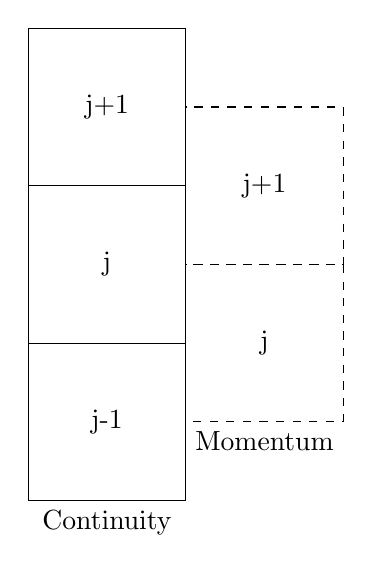
\begin{tikzpicture}
\draw (-2,-3) rectangle +(2,2);
\node[anchor=center] at (-1,-2) {j-1};
\draw (-2,-1) rectangle +(2,2);
\node[anchor=center] at (-1, 0) {j};
\draw (-2, 1) rectangle +(2,2);
\node[anchor=center] at (-1, 2) {j+1};
\draw[dashed] (-0,-2) rectangle +(2,2);
\node[anchor=center] at (1, -1) {j};
\draw[dashed] (-0, 0) rectangle +(2,2);
\node[anchor=center] at (1, 1) {j+1};
\node[anchor=north] at (-1, -3) {Continuity};
\node[anchor=north] at (1, -2) {Momentum};
\end{tikzpicture}
\end{center}
\end{figure}

Recalling the staggered grid from \sect{sect:topology}, the six scalar conservation laws, \eqref{eqn:conservation_of_ncg} -- \eqref{eqn:con_energy_liq}, are each integrated over the continuity volumes.
The assumption in these integrals is that the value of the conserved quantities and all thermodynamically related variables are constant within a given cell.
\fig{fig:constant_value} shows a graphical representation of this idea for a generic function $f(x)$ over several spatial continuity meshes.

\begin{figure}[ht]
\caption{Constant variable values within computational volumes.}
\label{fig:constant_value}
\begin{center}
Picture goes here.
\end{center}
\end{figure}

For illustrative purposes,  the \eqref{eqn:conservation_of_liq} will be integrated over a given volume, $j$, as shown in \fig{fig:single_volume}.

\begin{figure}[ht]
\caption{Single volume over which integration is done.}
\label{fig:single_volume}
\begin{center}
Picture goes here.
\end{center}
\end{figure}

Within a given channel, $k$, a given continuity volume has a constant cross-sectional area, $A_{c_{j}}$, and a length of $\Delta x_{j}$.
The cross-section area of the boundary between two continuity volumes is given by the cross-section area of the momentum volume at that boundary, $A_{m}$.

\begin{IEEEeqnarray}{lcl}
\int_{V_j}\frac{\partial \left(\alpha_l \rho_l \right)}{\partial t } & + & \nabla \cdot \left( \alpha_l \rho_l u_l \right) \mathrm{d}V = \int_{V_j} \left(-(1-\eta)\Gamma^{'''} - S^{'''} + s_{m,l}\right) \mathrm{d}V \nonumber \\
V_j \frac{\partial \left(\alpha_{l,j} \rho_{l,j} \right)}{\partial t } & = & -\int_{V_j}\nabla \cdot \left( \alpha_l \rho_l u_l \right) \mathrm{d}V -(1-\eta_j)\Gamma_j^{'''}V_j - S_j^{'''}V_j + s_{m,l,j}V_j \nonumber \\
V_j \frac{\partial \left(\alpha_{l,j} \rho_{l,j} \right)}{\partial t } & = & -A_{m,j}\left[\alpha_l \rho_l u_l \right]_{x_{j-\frac{1}{2}}}^{x_{j+\frac{1}{2}}} -(1-\eta_j)\Gamma_j^{'''}V_j - S_j^{'''}V_j + s_{m,l,j}V_j \nonumber \\
\label{eqn:spatially_discrete_liq_m_con}
V_j \frac{\partial \left(\alpha_{l,j} \rho_{l,j} \right)}{\partial t } & = & -A_{m,j}\left( <\alpha_l \rho_l>_{d,j+\frac{1}{2}} u_{l,j+1} - <\alpha_l \rho_l>_{d,j-\frac{1}{2}} u_{l,j} \right) \nonumber \\
& & -(1-\eta)\Gamma^{'''}V - S^{'''}V_j + s_{m,l}V_j
\end{IEEEeqnarray}

For the mass-flux terms evaluated on the continuity volume edge, the advected quantity is evaluated using a 1st order upwind method \cite{Tannehill1997}.
The velocity and cross-sectional area utilized in the continuity flux terms, $u_j$ and $A_{m,j}$, have the values defined at the center of the momentum volume that aligns with the edge of continuity volumes.
The sign of the velocity at the volume boundary determines the value of the donored quantity, $<a>_{d,j-\frac{1}{2}}$.
A generic formulation for this scheme is given by \eqref{eqn:upwind_donoring}.
The same general procedure is used for the other five scalar conservation equations.

\begin{equation}
\label{eqn:upwind_donoring}
<a>_{d, j-\frac{1}{2}} = \begin{cases} a_{j-1} &  u_j \geq 0 \\ a_{j} & u_j < 0 \end{cases}
\end{equation}

The three momentum conservation laws, \eqref{eqn:con_mom_liq} -- \eqref{eqn:con_mom_ent}, are integrated over their momentum volume.
The cross section area for a momentum volume, $A_{m,j}$, can be defined independently of the two cross-sectional areas of the adjoining continuity volumes.
The momentum flux terms, \eqref{eqn:momentum_flux_terms}, are treated similarly to the flux terms in the continuity equations.
\begin{equation}
\label{eqn:momentum_flux_terms}
-\min\left(A_{m,j}, A_{m,j+1}\right)\left[<\alpha_l \rho_l u_l>_{d} u_l\right]_{x_{j-\frac{1}{2}}}^{x_{j+\frac{1}{2}}}
\end{equation}
There are two primary differences.
First, the momentum area 
The second difference is that the velocity that is used to determine the origination of the donored quantity is the arithmetic mean of the velocities from the two adjacent momentum volumes, \eqref{eqn:average_advecting_vel}.

\begin{equation}
\label{eqn:average_advecting_vel}
u_{k,j+\frac{1}{2}} = \frac{1}{2}\left(u_{k,j} + u_{k, j+1}\right)
\end{equation}

\subsection{Temporal Approximations}
\label{subsect:temporal_approx}
Once the governing conservation equations have been spatially discretized utilizing the method outlined above, the temporal derivatives need to be numerically approximated.
Using the spatially discrete approximations defined in \sect{subsect:spatial_approx}, the temporally continuous differential equations,\eqref{eqn:conservation_equations}, are now semi-discrete approximations given by \eqref{eqn:temporal_semi_discrete}, where $\vec{G}$ now represents the spatially discrete version of $\vec{g}$.

\begin{equation}
\label{eqn:temporal_semi_discrete}
\frac{\partial \,\vec{y} }{\partial t} = \vec{G}(\vec{y}(t))
\end{equation}

Within COBRA, the temporal derivative is approximated by a one-step difference scheme, \eqref{eqn:simple_partial_t}.
Where the continuous time variables are now evaluated at discrete points, $t^0, t^1, \ldots, t^N$, where $t^0$ represents the initial conditions and $t^N$ represents the final time.
The term one-step refers to the fact that the temporal derivative involves only two consecutive points in time.

\begin{IEEEeqnarray}{rcl}
\int^{t^{n+1}}_{t^n}\frac{\partial \vec{y}}{\partial t}\mathrm{d}\tau & = & \int^{t^{n+1}}_{t^n}\vec{G}(\vec{y})\mathrm{d}\tau \nonumber \\
\vec{y}^{n+1} - \vec{y}^{n} & = & \int_{t^{n+1}}^{t^n}\vec{G}(\vec{y})\mathrm{d}\tau \nonumber  \\
\frac{\vec{y}^{n+1} - \vec{y}^{n}}{\int_{t^{n}}^{t^{n+1}}\mathrm{d} \tau} & = & \frac{\int_{t^{n+1}}^{t^n}\vec{G}(\vec{y})\mathrm{d}\tau}{\int_{t^{n}}^{t^{n+1}}\mathrm{d} \tau} \nonumber \\
\frac{\vec{y}^{n+1} - \vec{y}^{n}}{\Delta t} & = & \frac{\int_{t^{n+1}}^{t^n}\vec{G}(\vec{y})\mathrm{d}\tau}{\int_{t^{n}}^{t^{n+1}}\mathrm{d} \tau} \nonumber \\
\label{eqn:simple_partial_t}
\frac{\vec{y}^{n+1} - \vec{y}^{n}}{\Delta t} & = & \vec{G}(\vec{y}^{*})
\end{IEEEeqnarray}

The choice of how to approximate the temporal-average, $\vec{G}(\vec{y}^{*})$, is a factor that defines the eventual solution algorithm.
The commonly used approximations will be postponed for now. 

\subsection{Nonlinear Approximations}
\label{sect:nonlinear_approximations}

Given the system of discretized PDEs, \eqref{eqn:simple_partial_t}, nine independent parameters are required
Given that there are nine conservation equations, the choice of which nine variables are the independent parameters that will be solved for is another distinguishing characteristic of safety analysis codes.
The choice made in the COBRA sub-channel analysis codes is shown in \eqref{eqn:independent_variables}.

\begin{equation}
\label{eqn:independent_variables}
\vec{x} = [\alpha_{ncg}P_{ncg}, \alpha_g, P, \alpha_e, \alpha_gS h_v, (1 - \alpha_g) h_l, \dot{m}_g, \dot{m}_l, \dot{m}_e]^{T}
\end{equation}

The definition of $\dot{m}_k$ is given by \eqref{eqn:mom_dot}.

\begin{equation}
\label{eqn:mom_dot}
\dot{m}_k = \alpha_k \rho_k u_k A_m
\end{equation}

In the particular discretization utilized, there are several nonlinear terms that are to be evaluated implicitly.

For the two-phase flow equations of interest, the conserved variables at $t^{n+1}$ are nonlinear functions of the independent parameters.
These temporal nonlinearities exist in all numeric methods.
For those methods that has any implicit variables on the RHS, there are additional nonlinearities introduced.
In order to deal with these nonlinearities, there are two general branches of solution techniques.
A choice can be made to not resolve the nonlinearities, or an iterative procedure can be introduced to resolve the nonlinearities of interest.

\subsubsection{Newton's Method}
\label{subsubsect:newtons_method}
The primary method used to resolve the non-linearities in the governing equations is the use of a Newton's method \cite{Deuflhard2004}.
Newton's method is an optimization algorithm that is particularly well suited for discretized systems of PDEs.

\subsubsection{Single-shot Linearization}
\label{subsubsect:single_shot}
If the nonlinearities in the numeric method are not resolved.

%--------------------------------------------------------------------------------------------------------------------------------------------------------------------
%--------------------------------------------------------------------------------------------------------------------------------------------------------------------
%--------------------------------------------------------------------------------------------------------------------------------------------------------------------
%--------------------------------------------------------------------------------------------------------------------------------------------------------------------
%--------------------------------------------------------------------------------------------------------------------------------------------------------------------
%--------------------------------------------------------------------------------------------------------------------------------------------------------------------
%--------------------------------------------------------------------------------------------------------------------------------------------------------------------

\section{Solution Methods}
\label{sect:solution_techniques}

\subsection{Explicit}
\label{subsect:numerics_explicit}
The least computationally expensive method for temporally integrating the PDEs from \sect{subsect:governing_equations} is a simple fully explicit method.
The terminology explicit refers to the fact that the unknowns at $t^{n+1}$, $\vec{y}^{n+1}$, are function of the values at the present time $\vec{y}^{n}$ only.
The vector notation formulation for this method is given by \eqref{eqn:explicit}. 

\begin{equation}
\label{eqn:explicit}
\frac{ \vec{y}^{n+1} - \vec{y}^{n}}{\Delta t} = \vec{G}(\vec{y}^{n})
\end{equation}

The algorithmic implementation is shown in \alg{algo:explicit}.

\begin{algo}[H]
\caption{Explicit time-integration.}
\label{algo:explicit}
\setlength{\baselineskip}{0.625\baselineskip}
\begin{algorithmic}[1]
\Require $\vec{y}^{0}$ and $t^{0}$
\Set $n = 0$
\Loop \; Take a Time Step
    \State $t^{n+1} : = t^{n} + \Delta t$
    \Calculate $\vec{y}^{n+1} = \vec{y}^{n} + \Delta t \vec{G}(\vec{y}^n)$
\EndLoop{\;$n = n+1$}
\end{algorithmic}
\end{algo}

While this particular method is the least computationally expensive, it has a severe weakness in the context of the two-phase flow equations that are used in COBRA.
That weakness is the Courant-Friedrichs-Lewy (CFL) limit imposed upon the time step size, $\Delta t$.
The CFL limit is a relationship between the spatial and temporal discretization and the characteristic velocities of information propagation in the problem of interest \cite{LeVeque2007, Tannehill1997}.
For the case of \eqref{eqn:explicit}, the CFL limit is given in \eqref{eqn:cfl_explicit}.

\begin{equation}
\label{eqn:cfl_explicit}
\Delta t_j \lesssim \frac{\Delta x_j}{|u_j|+|c_j|}
\end{equation}

Where $c_j$ is the speed of sound and $u_j$ is the magnitude of a given phasic velocity at a given location within the domain.
$\Delta t_j$ is calculated at every point within the domain using the known local fluid conditions.
The $\Delta t$ chosen for the $t^{n} \rightarrow t^{n+1}$ time-step is the most restrictive value over the domain.
While the explicit method may provide for the least computational cost on a per-time-step basis, the number of time-steps required for a given problem will be much higher due to the restrictive CFL limitations.

\begin{equation}
\label{eqn:global_cfl}
\Delta t = \min_{j \in \Omega} \Delta t_j
\end{equation}

Stated in words, the maximum permissible time-step size for the explicit method is limited by the local speed of sound.
This limitation of the explicit method prompted the development of alternative methods that were capable of exceeding this limitation.

\subsection{Implicit}
\label{subsect:numerics_fully_implicit}
An alternative method for integrating \eqref{eqn:temporal_semi_discrete} is to use a fully implicit technique.
A fully-implicit formulation is one where $\vec{G}$ is function only of unknown variables, \eqref{eqn:implicit}.

\begin{equation}
\label{eqn:implicit}
\\vec{y}^{n+1} = \vec{y}^{n} + \Delta t \vec{G}(\vec{y}^{n+1})
\end{equation}

This particular formulation has the advantage of not being limited by a CFL number.
However, the solution of \eqref{eqn:implicit} is computationally expense as that $\vec{G}(\vec{y}^{n+1})$ is a highly nonlinear function requiring the use of nonlinear solvers to obtain a solution.
A discussion of nonlinear-solvers will be postponed for now.
The computational implementation of the fully-implicit method is presented in \alg{algo:implicit}.

\begin{algo}[H]
\caption{Implicit time-integration.}
\label{algo:implicit}
\setlength{\baselineskip}{0.625\baselineskip}
\begin{algorithmic}[1]
\Require $\vec{y}^{0}$ and $t^{0}$
\Set $n = 0$
\Loop \; Take a Time Step	
    \State $t^{n+1} : = t^{n} + \Delta t$
    \BlackBox Solve $\vec{y}^{n+1} = \vec{y}^{n} + \Delta t \vec{G}(\vec{y}^{n+1})$ for $\vec{y}^{n+1}$
\EndLoop{\;$n = n+1$}
\end{algorithmic}
\end{algo}

The solution to the full nonlinear system of equations is the most computationally expensive option available.
However, it provide for the fewest time steps required in a given problem.

\subsection{IMEX}
\label{subsect:temporal_imex}

The sonic CFL limitation of the fully explicit method, together with the high computational cost of the fully implicit method, led to the development of mixed implicit-explicit (IMEX) methods.
The development of IMEX methods was develop a method that was able to overcome the time-step limitations of the fully explicit method while keeping the added computational cost to a minimum.
The first IMEX solution method to be widely used was the semi-implicit method \cite{Liles1978}.


\subsubsection{Semi-Implicit}
\label{subsubsect:semi_implicit}
To obtain the semi-implicit formulation, the $\vec{G}$ in \eqref{eqn:temporal_semi_discrete} is modified and combined with \eqref{eqn:simple_partial_t} to produce \eqref{eqn:semi_implicit_MOL}.

\begin{equation}
\label{eqn:semi_implicit_MOL}
\frac{ \vec{y}^{n+1}_{j} - \vec{y}^{n}_{j}}{t^{n+1}-t^{n}} = \vec{G}(\vec{y}^{n},\vec{y}^{n+1})
\end{equation}

$\vec{G}$ is now a function of both known and unknown variables, hence the name semi-implicit. 
The particular formulation of the semi-implicit method is of importance to later sections, so a detailed description of the conservation laws from \sect{subsect:governing_equations} is provided in equation \eqref{eqn:semi_implicit_flux_terms}.

\begin{IEEEeqnarray}{lCl}
\label{eqn:semi_implicit_flux_terms}
2 & = & 2
\end{IEEEeqnarray}

\begin{algo}[H]
\caption{Semi-Implicit Linear Solution Algorithm}
\label{algo:semi_implicit}
\setlength{\baselineskip}{0.625\baselineskip}
\begin{algorithmic}[1]
\Require $\Vec{x}^{0}$ and $t^{0}$
\Set $n = 0$
\Loop \; Take a Time Step
    \Set $\vec{x}^{n}$
    \Calculate $\Delta t$
    \State $t^{n+1} : = t^{n} + \Delta t$
    \BlackBox Solve for $\vec{x}^{n+1}$
    \Calculate Courant Numbers
\EndLoop{\;$n = n+1$}
\end{algorithmic}
\end{algo}

\subsubsection{Nearly Implicit}
\label{subsubsect:numerics_nearly_implicit}
Another multi-stage method is called the Nearly-Implicit method \cite{Trapp1986}.

\subsubsection{SETS}
\label{subsubsect:numerics_sets}
An alternative formulation for the temporal derivative is a multi-stage method.
These methods involve predictor and corrector steps.

To overcome the material Courant limit exhibited by the semi-implicit method, several alternatives have been developed.
One alternative, known as the the stability-enhancing two-step method (SETS) \cite{Mahaffy1982}, eliminates the material Courant limit by introducing multiple iterative refinement of the solution within a given time-step.

%--------------------------------------------------------------------------------------------------------------------------------------------------------------------
%--------------------------------------------------------------------------------------------------------------------------------------------------------------------
%--------------------------------------------------------------------------------------------------------------------------------------------------------------------
%--------------------------------------------------------------------------------------------------------------------------------------------------------------------
%--------------------------------------------------------------------------------------------------------------------------------------------------------------------
%--------------------------------------------------------------------------------------------------------------------------------------------------------------------
%--------------------------------------------------------------------------------------------------------------------------------------------------------------------
\section{Domain Coupling}
\label{sect:code_coupling}
There are several options to couple the specialized capabilities of system analysis codes to the detailed physics of a sub-channel analysis code.
These methodologies, are constantly evolving.
The types of methods follow the layout of method of lines.

\subsection{Explicit}
\label{subsect:coupling_explicit}
The first coupling method proposed was explicit coupling.
This method involved passing information between two different codes at the beginning of a time-step.


\subsection{Semi-Implicit}
\label{subsect:coupling_semi_implicit}
The desire to overcome the instabilities outlined in the previous section, a semi-implicit coupling method was proposed that made use of Parallel Virtual Machine (PVM).
PVM is a piece of software developed for the purpose of passing information between programs running in parallel \cite{Geist1994}. 
The ability to pass information between software is key to the semi-implicit stuff. 

\subsection{Implicit}
\label{subsect:coupling_implicit}
The concept of implicitly coupling different physics is sufficiently attractive. 
%--------------------------------------------------------------------------------------------------------------------------------------------------------------------
%--------------------------------------------------------------------------------------------------------------------------------------------------------------------
%--------------------------------------------------------------------------------------------------------------------------------------------------------------------
%--------------------------------------------------------------------------------------------------------------------------------------------------------------------
%--------------------------------------------------------------------------------------------------------------------------------------------------------------------
%--------------------------------------------------------------------------------------------------------------------------------------------------------------------
%--------------------------------------------------------------------------------------------------------------------------------------------------------------------
\section{Temporal Convergence}
\label{sect:temporal_convergence}
The ability to predict the behavior of reactors during off-normal events is the key to the licensing and the operation of nuclear power plants.
Within the United States, this simulation capacity is provided by a relatively small number of main stream software suites, among which are the RELAP variants, COBRA variants, and MELCOR.
While each of these software products varies in their models and implementations, the underlying numeric techniques and capabilities are similar.

\subsection{Time Step Selection}
\label{subsect:time_step_selection}
BLARPER!
\subsection{Time Step Failure}
\label{subsect:time_step_failure}
There are two common methods for dealing with a potentially poor time-step in sub-channel codes: prediction and mitigation.
The predictive method is the less commonly applied of the two methods.
It uses information about the explicit portion of the nonlinear residual to identify situations where the linearization point may be poor.
In COBRA, this particular method is used only for the prediction of \ncg appearance.

Mitigation, the second method, is the more common and actively used strategy.
This strategy can be further subdivided into two categories: limiting and failure.
There is an extensive set of limiting criteria.
%--------------------------------------------------------------------------------------------------------------------------------------------------------------------
%--------------------------------------------------------------------------------------------------------------------------------------------------------------------
%--------------------------------------------------------------------------------------------------------------------------------------------------------------------
%--------------------------------------------------------------------------------------------------------------------------------------------------------------------
%--------------------------------------------------------------------------------------------------------------------------------------------------------------------
%--------------------------------------------------------------------------------------------------------------------------------------------------------------------
%--------------------------------------------------------------------------------------------------------------------------------------------------------------------
\section{Review}
\label{sect:review}
Marbles!
%--------------------------------------------------------------------------------------------------------------------------------------------------------------------
%--------------------------------------------------------------------------------------------------------------------------------------------------------------------
%--------------------------------------------------------------------------------------------------------------------------------------------------------------------
%--------------------------------------------------------------------------------------------------------------------------------------------------------------------
%--------------------------------------------------------------------------------------------------------------------------------------------------------------------
%--------------------------------------------------------------------------------------------------------------------------------------------------------------------
%--------------------------------------------------------------------------------------------------------------------------------------------------------------------
\section{Research Objective}
The objective of this research is the design, implementation, and evaluation of spatially selective nonlinear solution framework for reactor safety systems codes.
Specifically, an efficient and reliable solution method to the two-phase, three-field, fluid-dynamic system of coupled non-linear partial differential equations is sought.
The specific method should be capable of obtaining a consistent solution to the system of PDEs while also possessing.
\cite{Aktas1996}
The limiting behavior of nuclear reactors occurs during the end portion of a severe accident.
The primary point of investigation is the use of domain decomposition for the purpose of refining the solution to the nonlinear conservation within COBRA-IE.
The domain decomposition will take place utilizing a generic semi-implicit coupling method developed by \citet{Weaver2002}.
The ability to isolate a subdomain of the problem and increase ability of the software to resolve the complex nonlinear physics that occur near the quench front of a reflood transient.
This method will hopefully increase the predictive capabilities of safety analysis codes while keeping the computational overhead as low as reasonable possible.       % Chapter: Context of the problem.
\chapter{Preliminary Work}
\label{chap:prelim_work}
As preliminary work, several steps were taken to evaluate the validity of the proposed research.
In order to determine the effects of nonlinear convergence upon the timestep size insensitivity of a solution, the \cobra{} software was modified to enable an iterative global Newton's method.
A metric was developed for the evaluation of the nonlinear convergence of a timestep.
To aid in the development of the nonlinear convergence metric and the nonlinear solver, a novel operator-based scaling has been developed to obtain meaningful convergence thresholds.
The scaling of the nonlinear residual is typically done in an arbitrary fashion; a scaling factor that is intrinsically linked to the physics of interest was developed.
This scaling produces a non-dimensionalized residual whose magnitude is relative to the physical sources and sinks on a per equation basis. 
Two temporal convergence test problems were developed to show that the nonlinear convergence metric can identify situations where a timestep size insensitive simulation may not satisfy the discrete nonlinear equations.
%--------------------------------------------------------------------------------------------------------------------------------------------------------------------
%--------------------------------------------------------------------------------------------------------------------------------------------------------------------
%--------------------------------------------------------------------------------------------------------------------------------------------------------------------
%--------------------------------------------------------------------------------------------------------------------------------------------------------------------
%--------------------------------------------------------------------------------------------------------------------------------------------------------------------
%--------------------------------------------------------------------------------------------------------------------------------------------------------------------
%--------------------------------------------------------------------------------------------------------------------------------------------------------------------
\section{Nonlinear \cobra{} Implementation}
\label{sect:nl_cobra}  
The first stage of the preliminary work was to modify the \cobra{} software.
As obtained, the \cobra{} software used a single-shot linearization  of the semi-implicit method.
In order to evaluate the subdomain nonlinear refinement algorithm, \cobra{} was converted to include a fully iterative Newton solver based upon a linesearch globalization strategy.
When it is necessary to distinguish between the single-shot linearization algorithmic implementation of \cobra{} and the iterative nonlinear \cobra{} implementation, the former shall be referred to as the legacy solver and the latter as the nonlinear solver.
As such, the \cobra{} software needed to be modified to be able do the following:

\begin{itemize}
\item{Create a data framework for constructing vector quantities such as $\vec{x}^{k}$ and $\vec{F}$.}
\item{Correctly evaluate $\vec{F}(\vec{x}^{k})$ and $\vec{J}(x^{k})$.}
\item{Implement a globalization strategy for Newton's method.}
\end{itemize}

\cobra{} utilized a single-shot linearization for its solution technique.
As a result of that design decision, certain memory saving techniques were employed in the construction of the software that precluded the idea of more than one Newton step.
In particular, there was the implicit assumption within the software that the current Newton iterate, $\vec{x}^{n+1, 0}$, was the old-time variable $\vec{x}^{n}$.
This design decision required the vetting of all subroutines involved with the evaluation of the components of both the nonlinear residual and the Jacobian.
In addition, the assumption that $\vec{x}^{n+1, k} = \vec{x}^{n}$ produced source code that was inconsistent with an iterative Newton method.
The source code was modified to reflect the intended discretization of the governing conservation laws.
To do this, areas had to be identified where: there were implicit cancellation of terms, the new-time variables were used in place of old-time variables, and the old-time variables were used in place of new-time variables.
Where appropriate, the software was changed to reflect the distinction between old-time and iterate variables and to introduce terms that had been assumed to be equal to zero.

Once the appropriate variables were used for the evaluation of the nonlinear residuals and the Jacobian, a Newton loop was introduced to allow multiple Newton steps.
\alg{alg:nl_cobra} contains the current algorithmic implementation of the nonlinear semi-implicit method.

\begin{algo}[H]
\setlength{\baselineskip}{0.625\baselineskip}
\begin{algorithmic}[1]
\Require $\vec{x}^{0}$ and $t^{0}$
\Set $n = 0$
\Loop \; Transient Loop
    \State $t^{n+1} : = t^{n} + \Delta t$
    \State $k = 0$
    \Define $\vec{x}^{n+1,0}$
	\Calculate $\vec{F}(\vec{x}^{n+1,0})$ and $\vec{J}(\vec{x}^{n+1,0})$
    \Loop \; Newton Loop
		\Calculate $\vec{\delta x} = - \vec{J}^{-1}\cdot\vec{F}$
		$j = 0$		
		\Calculate $\vec{x}^{n+1,k+1,j}$
		\Calculate $\vec{F}(\vec{x}^{n+1,k+1,j})$
		\Loop \; Globalization Loop
			\If{ Globalization loop termination criteria not met}
				\Calculate $\lambda_j$
				\Calculate $\vec{x}^{n+1,k+1,j+1} = \vec{x}^{n+1,k} + \lambda \vec{\delta x}$
				\Calculate $\vec{F}(\vec{x}^{n+1,k+1,j+1})$
				\State $j = j + 1$			
			\Else
				\Calculate $\vec{J}(\vec{x}^{n+1,k+1,j})$
				\Exit Globalization Loop
			\EndIf
		\EndLoop			
		\If{ Newton loop termination criteria met}
			\Exit Newton Loop
		\EndIf
	\EndLoop
	\State $n = n + 1$
\EndLoop
\end{algorithmic}
\caption{Nonlinear \cobra{} algorithm.}
\label{alg:nl_cobra}
\end{algo}

In \alg{alg:nl_cobra}, there are three steps that require discussion.
First is the Newton Loop termination criteria.
There are three Newton loop termination mechanisms, listed below.

\begin{enumerate}
\item{$k > k_{\,\text{MAX}}$}
\item{$||(\vec{S}^{k+1})^{-1}\vec{F}^{k+1}||_{\infty} \leq F_{\text{ABS}}$}
\item{$||(\vec{D}^{k+1})^{-1}\vec{\delta x}^{k}||_{\infty} \leq \delta_{\text{ABS}}$}
\end{enumerate}

Current values for $k_{\,\text{MAX}}$, $F_{\text{ABS}}$ and $\delta_{\text{ABS}}$ are $35$, $1.0$E$-05$, and $1.0$E$-10$, respectively.
The scaling vectors, $\vec{S}$ and $\vec{D}$, will be addressed later.

The second is the globalization loop termination criteria.
The globalization strategy implemented in \cobra{} is a linesearch algorithm \cite{Dennis1996}.
The two globalization loop termination criteria are:

\begin{enumerate}
\item{$\frac{1}{2}||\vec{F}^{k+1, j}||^{2}_{2} < \frac{1}{2}||\vec{F}^{k}||^{2}_{2} - \alpha ||\vec{F}^{k}||^{2}_{2}$ }
\item{$||\lambda_{j+1} \vec{\delta x}^{k}||_{\infty} < \delta_{\text{abs}}$}
\end{enumerate}

The third point requiring discussion is the calculation of the Newton update vector.
If neither of the loop termination criteria are met, then a step-length parameter, $\lambda_j$, is calculated.
On the first pass through the globalization loop within a given Newton step, a quadratic backtracking model is adopted.
On subsequent passes, a cubic-backtracking model is used.
 
Since vector forms of the nonlinear residual and the independent parameters are used in determining nonlinear convergence and in the globalization algorithm, they needed to be easily manipulated.
A subroutine was written to gather the discrete variables of the independent parameters into a single vector.
Additional source code modifications were necessary to construct and gather the components of the nonlinear residual.

The development of the nonlinear solver within \cobra{} took place under strict quality assurance guidelines.
At every step of the development, the legacy solver was required to maintain the same solution.
This verification was dependent upon a larger number of verification and assessment problems.
The output of the unmodified \cobra{} and the modified \cobra{} software was compared to machine precision.
It was required that either the results of the two simulations be identical or that the reason for the difference be identified and understood.
The \cobra{} software has the ability to repeat a time-step.
As such, it was required that the backup capabilities continued to work while nonlinear solver was being implemented.
Additionally, testing was done to ensure that the ability to restart the software mid-simulation was unaffected.
While adding time to the development cycle, the overhead of the quality assurance procedures ensured that the legacy solver could continue to be used for design purposes.

%--------------------------------------------------------------------------------------------------------------------------------------------------------------------
%--------------------------------------------------------------------------------------------------------------------------------------------------------------------
%--------------------------------------------------------------------------------------------------------------------------------------------------------------------
%--------------------------------------------------------------------------------------------------------------------------------------------------------------------
%--------------------------------------------------------------------------------------------------------------------------------------------------------------------
%--------------------------------------------------------------------------------------------------------------------------------------------------------------------
%--------------------------------------------------------------------------------------------------------------------------------------------------------------------
\section{Operator-Based Scaling}
\label{sect:operator_scaling}
In order to determine the degree to which a state vector, $\vec{x}$, satisfies \eqref{eqn:conservation_equations}, the use of the nonlinear residual is required.
However, due to the units of the residuals for the different conservation equations, their values can vary by orders of magnitude. 
For a given continuity volume, the nonlinear residual will have six components: four for the conservation of mass and two for the conservation of energy.
For each momentum volume, the three conservation of momentum equations will form the three components of the nonlinear residual.
These residuals have the units of the conserved quantities for their corresponding PDEs; \tab{tab:scaling_units_scales} shows the units for the different conservation equations.

\begin{table}[ht]
\centering
\begin{tabular}{@{}l c r @{}} \toprule
Residual & Units \\
\midrule
Conservation of the \NCG{} Field Mass                  & [ lb$_m$ ] \\
Conservation of the Continuous Liquid Water Field Mass & [ lb$_m$ ] \\
Conservation of the Entrained Liquid Water Field Mass  & [ lb$_m$ ] \\
Conservation of the Water Vapor Field Mass             & [ lb$_m$ ] \\
Conservation of the Gaseous Phase Enthalpy             & [ BTU ]    \\
Conservation of the Liquid Phase Enthalpy              & [ BTU ]    \\
Conservation of the Continuous Liquid Field Momentum   & [ $\frac{\text{lb}_{\text{m}} \text{ft}}{\text{s}}$ ] \\
Conservation of the Entrained Liquid Field Momentum & [ $\frac{\text{lb}_{\text{m}} \text{ft}}{\text{s}}$ ] \\
Conservation of the Gaseous Phase Momentum & [ $\frac{\text{lb}_{\text{m}} \text{ft}}{\text{s}}$ ] \\
\bottomrule  
\end{tabular}
\caption{Residuals and their units.}
\label{tab:scaling_units_scales}
\end{table}

Due to the range of magnitudes of these residuals it is important to choose a proper scaling factor to ensure that the convergence of each equation is relative to their magnitude.
A challenge that has been addressed in this work is the development of a method for scaling of these residuals that is based upon the physics of interest during a timestep.
In constructing this scaling factor it was determined that the following characteristics were desirable:

\begin{itemize}
\item{$(S_{i}^{k})^{-1} F^{k}_i \approx 1$ when $\vec{x}^{k}$ is a "poor" solution.}
\item{$(S_{i}^{k})^{-1} F^{k}_i \rightarrow 0$ when phase $i$ disappears.}
\item{$0 \leq \abs{(S_{i}^{k})^{-1} F^{k}_{i}} \leq 1 $ for all values of $\vec{x}^{k}_i$.}
\end{itemize}

The scaling used in this work is an operator-based approach.
The governing PDEs can be viewed as a collection of operators, both linear and nonlinear, acting upon the vector of independent parameters.
The summation of these operators must balance to zero for the nonlinear equation to be satisfied.

To illustrate the scaling procedure, we shall consider the discrete conservation of continuous liquid mass \eqref{eqn:si_mass_liq}.
The residual for \eqref{eqn:si_mass_liq} would be \eqref{eqn:res_mass_liq}.

\begin{equation}
\label{eqn:res_mass_liq}
F_{m,l} = \Delta t \left[ V_c \frac{\left(\alpha_l \rho_l \right)^{n+1} - \left(\alpha_l \rho_l \right)^{n}}{\Delta t} + \sum_{NK}\left( <\alpha^n_l \rho^n_l>^{n}_{d} u^{n+1}_l  \cdot \vec{\bar{A}}\right) + \left[(1-\eta)\Gamma + S \right]^{n+1}\right]
\end{equation}

In this equation there are five physically meaningful quantities: the temporal difference, the mass flowing into  the volume, the mass flowing out of the volume, the mass exchange with the gaseous phase, and the mass exchange with the entrained liquid field.

The scaling chosen for this residual is shown by \eqref{eqn:scaling_factor}.
\begin{equation}
\label{eqn:scaling_factor}
S_{m,l} = \Delta t \left[ V_c \abs{\frac{\left(\alpha_l \rho_l \right)^{n+1} - \left(\alpha_l \rho_l \right)^{n}}{\Delta t}} + \sum_{NK}\abs{\left( <\alpha^n_l \rho^n_l>^{n}_{d} u^{n+1}_l  \cdot \vec{\bar{A}}\right)} + \left[\abs{(1-\eta)\Gamma} + \abs{S} \right]^{n+1}\right]
\end{equation}

This scaling creates a relative measure of the nonlinear residual when compared to the magnitude of the physics involved in the process.
The other mass, energy, and momentum equations each have similarly defined scaling factors for their respective residuals.
For convergence testing in the nonlinear version of \cobra{} and residual evaluation during the legacy mode, the scaled nonlinear residual is used.

The issue of phase transition was considered during this work.
Since \cobra{} does not actually transition the governing equations to those for single-phase flow, there will always be a nonlinear residual for those phases that are approximately absent.
It was determined that the effects of maintaining a depleted phase in the system of equations when solving the nonlinear problem created a unique issue.
The unscaled residuals would be on the order of machine round-off.
The operator based scaling factors for these residuals would also be within orders of magnitude of machine round-off.
This created the situation where the scaled nonlinear residual for the depleted field would be of $\mathcal{O}$(1).
These depleted residuals would dominate the determination of convergence.
To overcome this deficiency it was determined that when a phase or field began to deplete, the scaling factor would be scaled up to create an artificial decrease in the residual to counter the artificial presence of the depleted field.
This scaling is shown by \eqref{eqn:scaling_factor_small}.

\begin{equation}
\label{eqn:scaling_factor_small}
S_k = \max[1.0, \left(C_1 \frac{\alpha_{k,\text{MIN}}}{\alpha_k}\right)^{C_2} ] S_k
\end{equation}

For this work, the constant $C_1$ was set equal to 100, and the exponent $C_2$ was set equal to 6.
This particular phase transition scaling produced the regular operator scaling factor when the volume fraction of a phase is at least two orders of magnitude greater than the minimum volume fraction for that phase.
This drove the scaled residuals for phases that were nominally not present to zero.
The original coding of \cobra{} has a minimum volume fraction of $\alpha_{k,\text{MIN}}$ = 1.0E-6.
For the work performed here, that value was reduced to $\alpha_{k,\text{MIN}}$ = 1.0E-9.

%--------------------------------------------------------------------------------------------------------------------------------------------------------------------
%--------------------------------------------------------------------------------------------------------------------------------------------------------------------
%--------------------------------------------------------------------------------------------------------------------------------------------------------------------
%--------------------------------------------------------------------------------------------------------------------------------------------------------------------
%--------------------------------------------------------------------------------------------------------------------------------------------------------------------
%--------------------------------------------------------------------------------------------------------------------------------------------------------------------
%--------------------------------------------------------------------------------------------------------------------------------------------------------------------
\section{Convergence}
\label{sect:temporal_convergence}

An important factor in thermal-hydraulic safety analysis is the temporal convergence of the solution.
A definition for a temporally converged solution is required.
In theory, a temporally converged solution is one where the local truncation error due to the discrete approximation of the temporal integral is orders of magnitude below both the engineering scales of interest and precision of the physical models being used in the simulation.
Unfortunately, the precise measurement of the error in a simulation requires that an analytic solution be available for comparison.
During the simulation of physically realistic systems, there is rarely an analytic solution against which to compare.
This situation requires a slightly different definition of a temporally converged solution --- a definition that does not depend upon accurately measuring the local truncation error.

An alternative definition for temporal convergence could be ``as the timestep size is reduced, the change in the solution is small enough."
While commonly used, this definition is subjective.
Traditionally, ``change in solution" is addressed in a very qualitative manner.
Engineering judgment of which parameters of the solution are of interest is required.
These parameters may include items of regulatory concern such as peak clad temperature or peak system pressure.
Examining only engineering parameters of interest is a weakness.
This locality means that the entire solution domain is not being considered.
Depending upon the context in which the work is being done, the degree of ``small enough" may be nothing more than looking at a graph of the parameter of interest and using engineering judgment to say that ``those two graphs look about the same."
In some cases, a more quantifiable measure may be used.
An example of a quantifiable metric would be if two simulations with different \dtmax{} are classified as dissimilar if the two solutions produce a ``calculated peak fuel cladding temperature different by more than $50\,^{\circ}\mathrm{F}$" \cite{CFR10}.

While it may be that the change in the chosen parameters of interest does not exceed the limits placed upon it as the timestep size is refined, that behavior does not imply that the solution obtained is the solution to the discrete nonlinear problem.
A metric that can quantify the degree to which the obtained solution satisfies the nonlinear system of equations would be of great value.
The previously mentioned work into nonlinear convergence shows that a solution may be timestep size insensitive but not be the converged solution of the discretized problem \cite{Knoll2001}.
If the nonlinearities of the discrete governing equations are not resolved, then the temporal convergence rate can be degraded.
This degradation can produce results that qualitatively appear to be converged due to an almost zeroth order of temporal accuracy.
In practice, the timestep size insensitivity of a solution is often interpreted as temporal convergence.
This apparent temporal convergence, or timestep size insensitivity, of the solution may not be a result of reaching the solution to the discretized nonlinear equations, but instead could be indicative of the degraded order of accuracy due to the failure to resolve the nonlinearities at each timestep.
To determine if the timestep size insensitive transient solution is both timestep size insensitive and an accurate solution to the nonlinear problem, it is necessary to examine the nonlinear convergence of the system as an issue separate from the temporal-convergence.

The norm of the scaled residual from \sect{sect:operator_scaling} provides a well-scaled metric for instantaneous nonlinear convergence at any given time in the simulation.
The residual vector norm is divided by the number of equations in the residual to provide an average residual value per equation.
This equation-averaged scaled residual provides a metric for determining the degree of nonlinear convergence at any timestep in the simulation.
The natural extension of this metric to transient problems would be a temporal integral, \eqref{eqn:trans_res_simple}, of said norm.

\begin{equation}
\label{eqn:trans_res_simple}
R = \int_{t^{0}}^{t^{N}} ||\vec{F}(\tau)||_2 \,\mathrm{d} \tau
\end{equation}

Given the bounds of the scaled residual it was considered desirable to have a similarly scaled transient residual.
The transient residual in \eqref{eqn:trans_res_simple} possesses a dependence upon the number of timesteps taken.
To remove this dependence, a temporal average was instead investigated, \eqref{eqn:trans_res_ave}.

\begin{equation}
\label{eqn:trans_res_ave}
\tilde{R} = \frac{\int_{t^{0}}^{t^{N}} ||\vec{F}(\tau)||_2 \,\mathrm{d} \tau}{t^{N} - t^{0}}
\end{equation}

This metric possesses the desirable bounds $0 \leq R \leq 1$.
Other weighted temporal integrals were considered, such as a simple moment about $t^{0}$, \eqref{eqn:trans_res_mom}.
However, this moment has the disadvantage of weighting the latter portion of the transient greater than the early portion.

\begin{equation}
\label{eqn:trans_res_mom}
\tilde{R}_{\text{M}} = \frac{\int_{t^{0}}^{t^{N}} \,\tau\,||\vec{F}(\tau)||_2 \,\mathrm{d} \tau}{\int_{t^{0}}^{t^{N}} \,\tau \,\mathrm{d} \tau}
\end{equation}

%--------------------------------------------------------------------------------------------------------------------------------------------------------------------
%--------------------------------------------------------------------------------------------------------------------------------------------------------------------
%--------------------------------------------------------------------------------------------------------------------------------------------------------------------
%--------------------------------------------------------------------------------------------------------------------------------------------------------------------
%--------------------------------------------------------------------------------------------------------------------------------------------------------------------
%--------------------------------------------------------------------------------------------------------------------------------------------------------------------
%--------------------------------------------------------------------------------------------------------------------------------------------------------------------
\section{Numerical Experiments}
\label{sect:numerical_experiments}

In order to evaluate the interplay between the nonlinear convergence and temporal convergence, two test problems were constructed.
These tests problems were designed to answer the following two questions.

\begin{enumerate}
\item{Does the legacy solver have a converged timestep size insensitive solution similar to that produced by the nonlinear solver for simple problems?}
\item{Do the nonlinear convergence metrics provide a quantifiable measure for the nonlinear convergence of a timestep size insensitive solution?}
\end{enumerate}

\subsection{Geometry}
\label{subsect:experimental_geometry}
For both of the test problems, the same computational geometry was used;  \fig{fig:exp_geometry} represents the experimental geometry.
Each block represents a single continuity cell with a height of 4 [in].
The total height of the channel is 48 [in].
Each continuity cell has a cross-sectional area of 4 [in$^2$].
The red block at the top of the channel represents a boundary cell where the pressure and enthalpy are specified.
It represents an infinite reservoir filled with a fluid at a specified thermodynamic state.
The red triangle represents a specified flow at the bottom edge of the first continuity cell. 

\begin{figure}[h!t]
\begin{center}
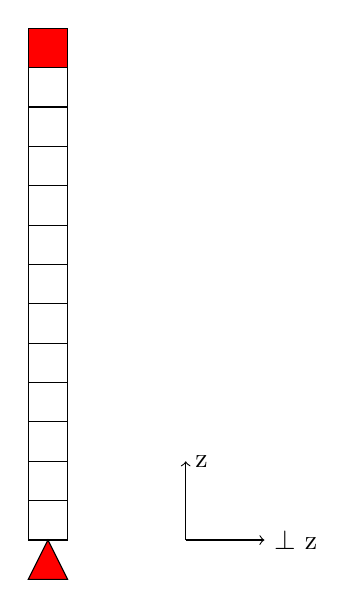
\begin{tikzpicture}
\foreach \x in {1,..., 12} \draw(0, 0.5*\x-0.5) rectangle +(.5,.5);
\filldraw[fill=red] (0, 6) rectangle +(.5,.5); 
\filldraw[fill=red] (0, -0.5) -- (0.25, 0) -- (0.5, -0.5) -- cycle;
\draw[->] (2,0) -- (2, 1) node[anchor=west] {z};
\draw[->] (2,0) -- (3, 0) node[anchor=west] {$\perp$ z};
\end{tikzpicture}
\end{center}
\caption{Geometry for test problems.}
\label{fig:exp_geometry}
\end{figure}

\subsection{Initial and Boundary Conditions}
\label{subsect:ic_bc}

The two problems, while having the same geometry, are different in their dominant physics.
One problem was designed to simulate single-phase, single-field continuous liquid flow in a standpipe.
This problem will be referred to as the single-phase problem.
The second problem was designed such that high-pressure liquid flashes into steam as it enters a standpipe initially filled with saturated vapor at a much lower pressure, known hereafter as the flashing problem.

Table \ref{tab:ic} provides the initial conditions for the two problems.
The pressure, enthalpy, and volume-fractions for the different fields allow for a complete description of the continuity variables.
The initial velocities are set to zero.

\begin{table}[ht]
\centering
\begin{tabular}{@{}lr@{.}lr@{.}lr@{.}lr@{.}lr@{.}l@{}} \toprule
\multirow{2}{*}{Problem} & \multicolumn{2}{c}{Pressure} & \multicolumn{2}{c}{Enthalpy}             & \multicolumn{2}{c}{$\alpha_g$} & \multicolumn{2}{c}{$\alpha_l$} & \multicolumn{2}{c}{$\alpha_e$} \\ 
                         & \multicolumn{2}{c}{[psia]} & \multicolumn{2}{c}{$[\frac{\text{BTU}}{\lbm{}}]$} & \multicolumn{2}{c}{[-]}      & \multicolumn{2}{c}{[-]}      & \multicolumn{2}{c}{[-]}      \\ \midrule
Single-Phase             &  200&0                       &  355&5                                   & 0&0                            & 1&0                            & 0&0 \\
Flashing                 &  200&0                       & 1198&3                                   & 1&0                            & 0&0                            & 0&0 \\ \bottomrule  
\end{tabular}
\caption{Initial conditions for test problems.}
\label{tab:ic}
\end{table}

Each of the problems has a specified pressure-enthalpy boundary condition at the top of the stand pipe and a flow-enthalpy boundary condition at the inlet of the domain.
Table \ref{tab:bc_pe} contains the pressure, enthalpy, and composition of the pressure-enthalpy reservoir. 

\begin{table}[ht]
\centering
\begin{tabular}{@{}lr@{.}lr@{.}lr@{.}lr@{.}lr@{.}l@{}} \toprule
\multirow{2}{*}{Problem} & \multicolumn{2}{c}{Pressure} & \multicolumn{2}{c}{Enthalpy}             & \multicolumn{2}{c}{$\alpha_g$} & \multicolumn{2}{c}{$\alpha_l$} & \multicolumn{2}{c}{$\alpha_e$} \\ 
                         & \multicolumn{2}{c}{[psia]} & \multicolumn{2}{c}{$[\frac{\text{BTU}}{\lbm{}}]$} & \multicolumn{2}{c}{[-]}      & \multicolumn{2}{c}{[-]}      & \multicolumn{2}{c}{[-]}      \\ \midrule
Single-Phase             &  200&0                       &  355&5                                   & 0&0                            & 1&0                            & 0&0 \\
Flashing                 &  200&0                       & 1198&3                                   & 1&0                            & 0&0                            & 0&0 \\ \bottomrule  
\end{tabular}
\caption{The pressure-enthalpy outlet boundary conditions for test problems.}
\label{tab:bc_pe}
\end{table}

The flow-enthalpy boundary condition describes the thermodynamic state of the inflowing fluid and its flow rate.
Table \ref{tab:bc_fe} describes the inlet boundary condition for the two problems.

\begin{table}[ht]
\centering
\begin{tabular}{@{}lr@{.}lr@{.}lr@{.}lr@{.}lr@{.}l@{}} \toprule
\multirow{2}{*}{Problem} & \multicolumn{2}{c}{Pressure} & \multicolumn{2}{c}{Enthalpy}             & \multicolumn{2}{c}{$\alpha_g$} & \multicolumn{2}{c}{$\alpha_l$} & \multicolumn{2}{c}{$\alpha_e$} \\ 
                         & \multicolumn{2}{c}{[psia]} & \multicolumn{2}{c}{$[\frac{\text{BTU}}{\lbm{}}]$} & \multicolumn{2}{c}{[-]}      & \multicolumn{2}{c}{[-]}      & \multicolumn{2}{c}{[-]}      \\ \midrule
Single-Phase             &  200&0                       &  355&5                                   & 0&0                            & 1&0                            & 0&0 \\
Flashing                 & 1000&0                       &  542&6                                   & 1&0                            & 0&0                            & 0&0 \\ \bottomrule  
\end{tabular}
\caption{The flow-enthalpy inlet boundary conditions for test problems.}
\label{tab:bc_fe}
\end{table}

The specified mass flow, $\dot{m}(t)$, at the bottom of the channels is the same for both problems. 
This time-dependent function is given by \eqref{eqn:bc_time_func_single}.

\begin{equation}
\label{eqn:bc_time_func_single}
\dot{m}(t) = \left\{
\begin{array}{cclrcll}
 0.0           & [\frac{ \lbm{} }{\text{s}}] & , &                & t & \leq 1 & [\text{s}] \\
 0.5 ( t - 1)  & [\frac{ \lbm{} }{\text{s}}] & , & 1\; [\text{s}] < & t & \leq 2 & [\text{s}] \\
 0.5           & [\frac{ \lbm{} }{\text{s}}] & , &                & t & > 2    & [\text{s}]
\end{array}\right.
\end{equation}

Both problems adjust their initial pressure distribution to account for hydrostatic head, which is not specified in the input files.
The \cobra{} input files for both problems can be found in \app{app:input_decks}.

\subsection{Procedure}
\label{subsect:procedures}

The two problems were set up so that the maximum allowable timestep was varied.
Each problem was run with the following maximum allowable timesteps: 1 [s], 0.1 [s], 0.01 [s], 0.001 [s], 0.0001 [s], and 0.00001 [s]. 
For the legacy runs, the scaled residuals were evaluated after a single Newton step, $\vec{F}(\vec{x}^{1})$.
For the nonlinear runs, the scaled nonlinear residuals were evaluated at the end of the Newton-loop.
The nonlinear convergence criteria used in the nonlinear solver are described in \sect{sect:nl_cobra}.
The temporal convergence metric was evaluated during post-processing.
In total, there were twenty-four simulations run.
The two different problems were each run at six different maximum timestep sizes on each of the two versions of \cobra{}.

\subsection{Results}
\label{subsect:results}

The results from the simulation runs will now be analyzed to determine the impact of nonlinear convergence upon time-step size sensitivity.
The solutions produced by both solvers will be compared to determine the efficacy of the residual metric in determining the validity of the nonlinear solution.  

Of the twenty-four simulations run, the legacy solver solution of the flashing problem with a \dtmax{} of 1 [s] failed to run to completion.
The timestep limiting procedure outlined in  \sect{sect:algorithmic_concerns} was unable to prevent too large a change in the independent parameters by reducing the timestep.
This caused the problem to try to run below the minimum allowable timestep size, which resulted in the software aborting.
However, the nonlinearly convergent \cobra{} was able to run at a \dtmax{} of 1 [s].
Both versions of \cobra{} are subject to the same limits on change of independent variables.

For the flashing problem, the parameter of interest for temporal convergence testing is $\alpha_g$ at 2 [in] from the inlet of the stand pipe.
\fig{fig:flashing_1em1} shows the gaseous volume fraction 2 [in] from the inlet of the stand pipe as a function of time for a \dtmax{} of 1.0E-1 [s] for both the legacy and the nonlinear solvers.

%\begin{figure}[h!t]
%\centering
%\subfloat[Solution with \dtmax{} = 1.0E-1 {[s]}]{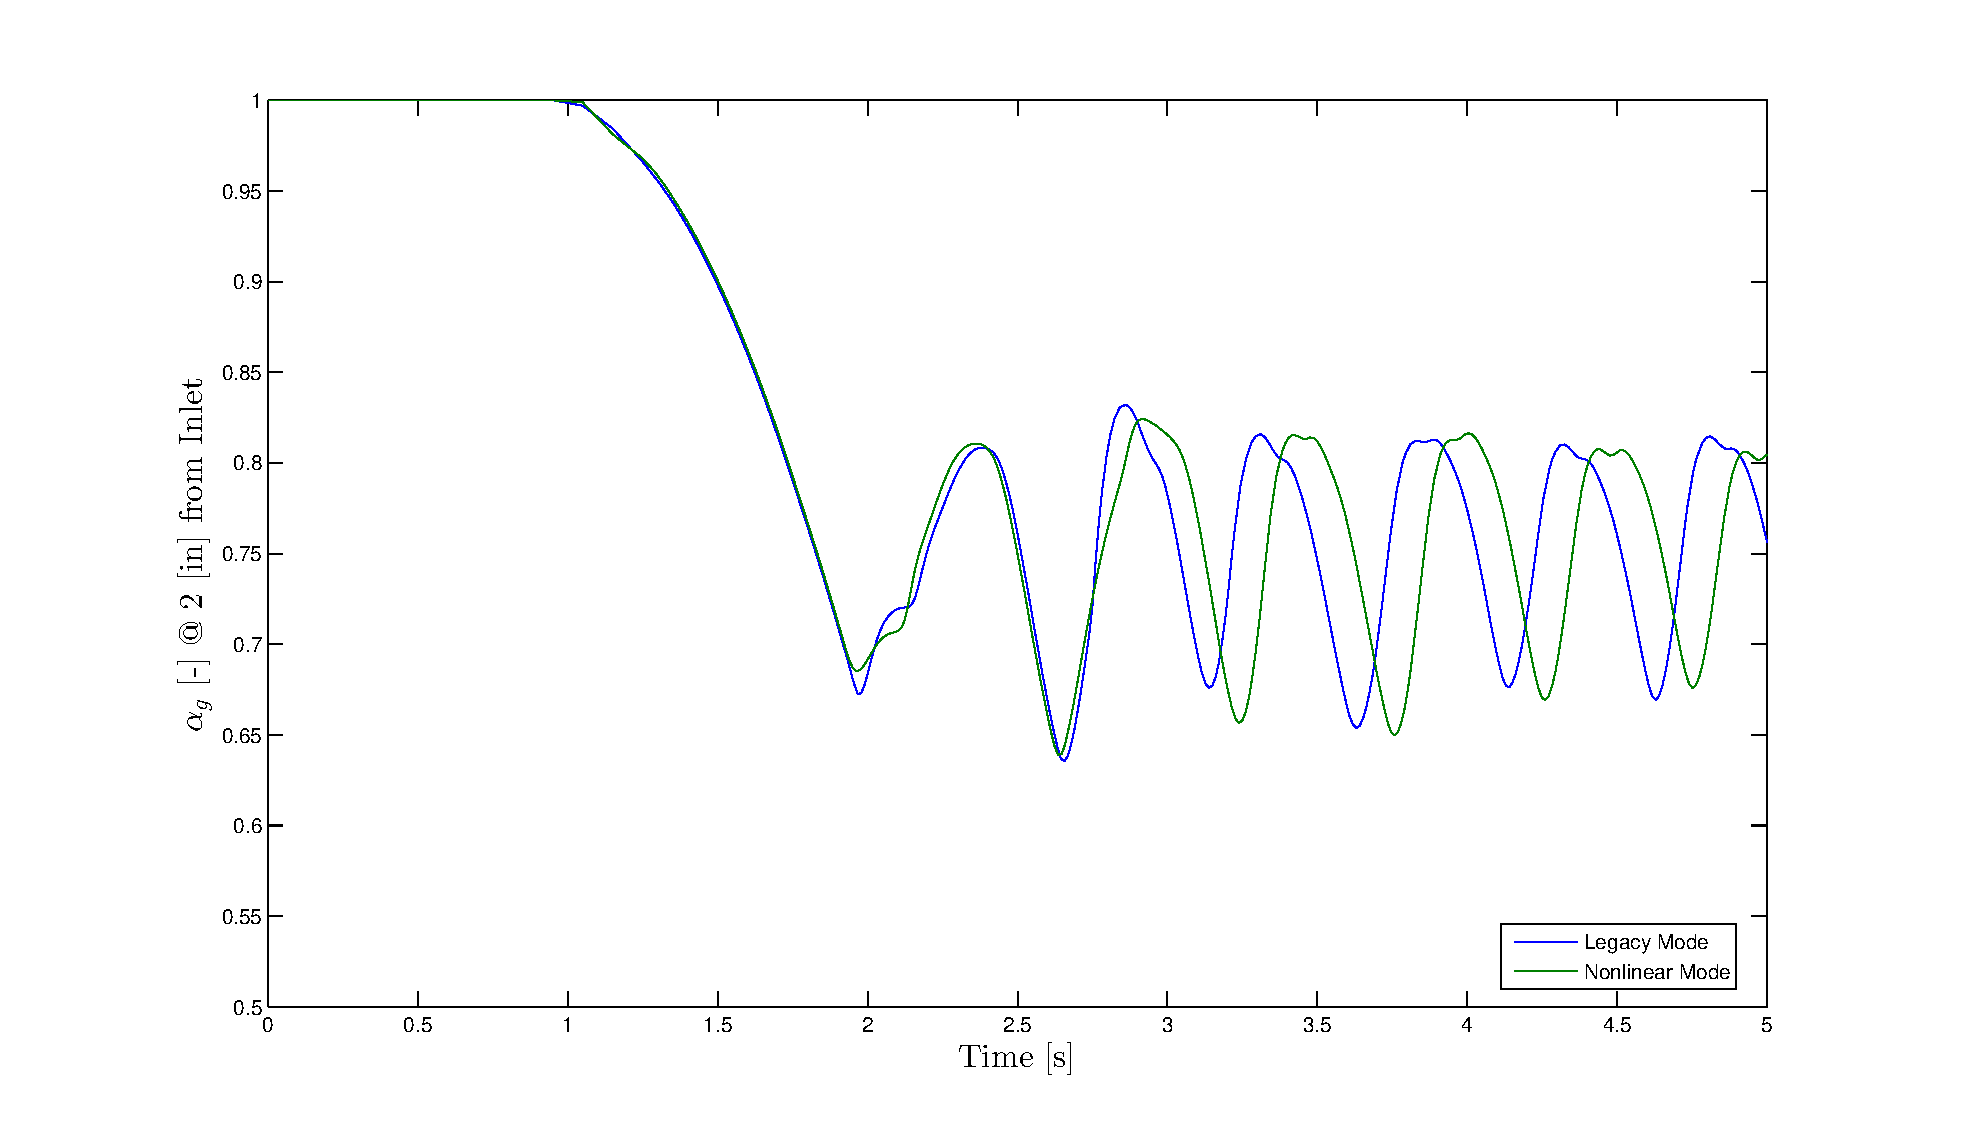
\includegraphics[width=0.49\textwidth]{images/flashing_1em1.eps}
%\label{fig:flashing_1em1}}
%\subfloat[Solution with \dtmax{} = 1.0E-5 {[s]}]{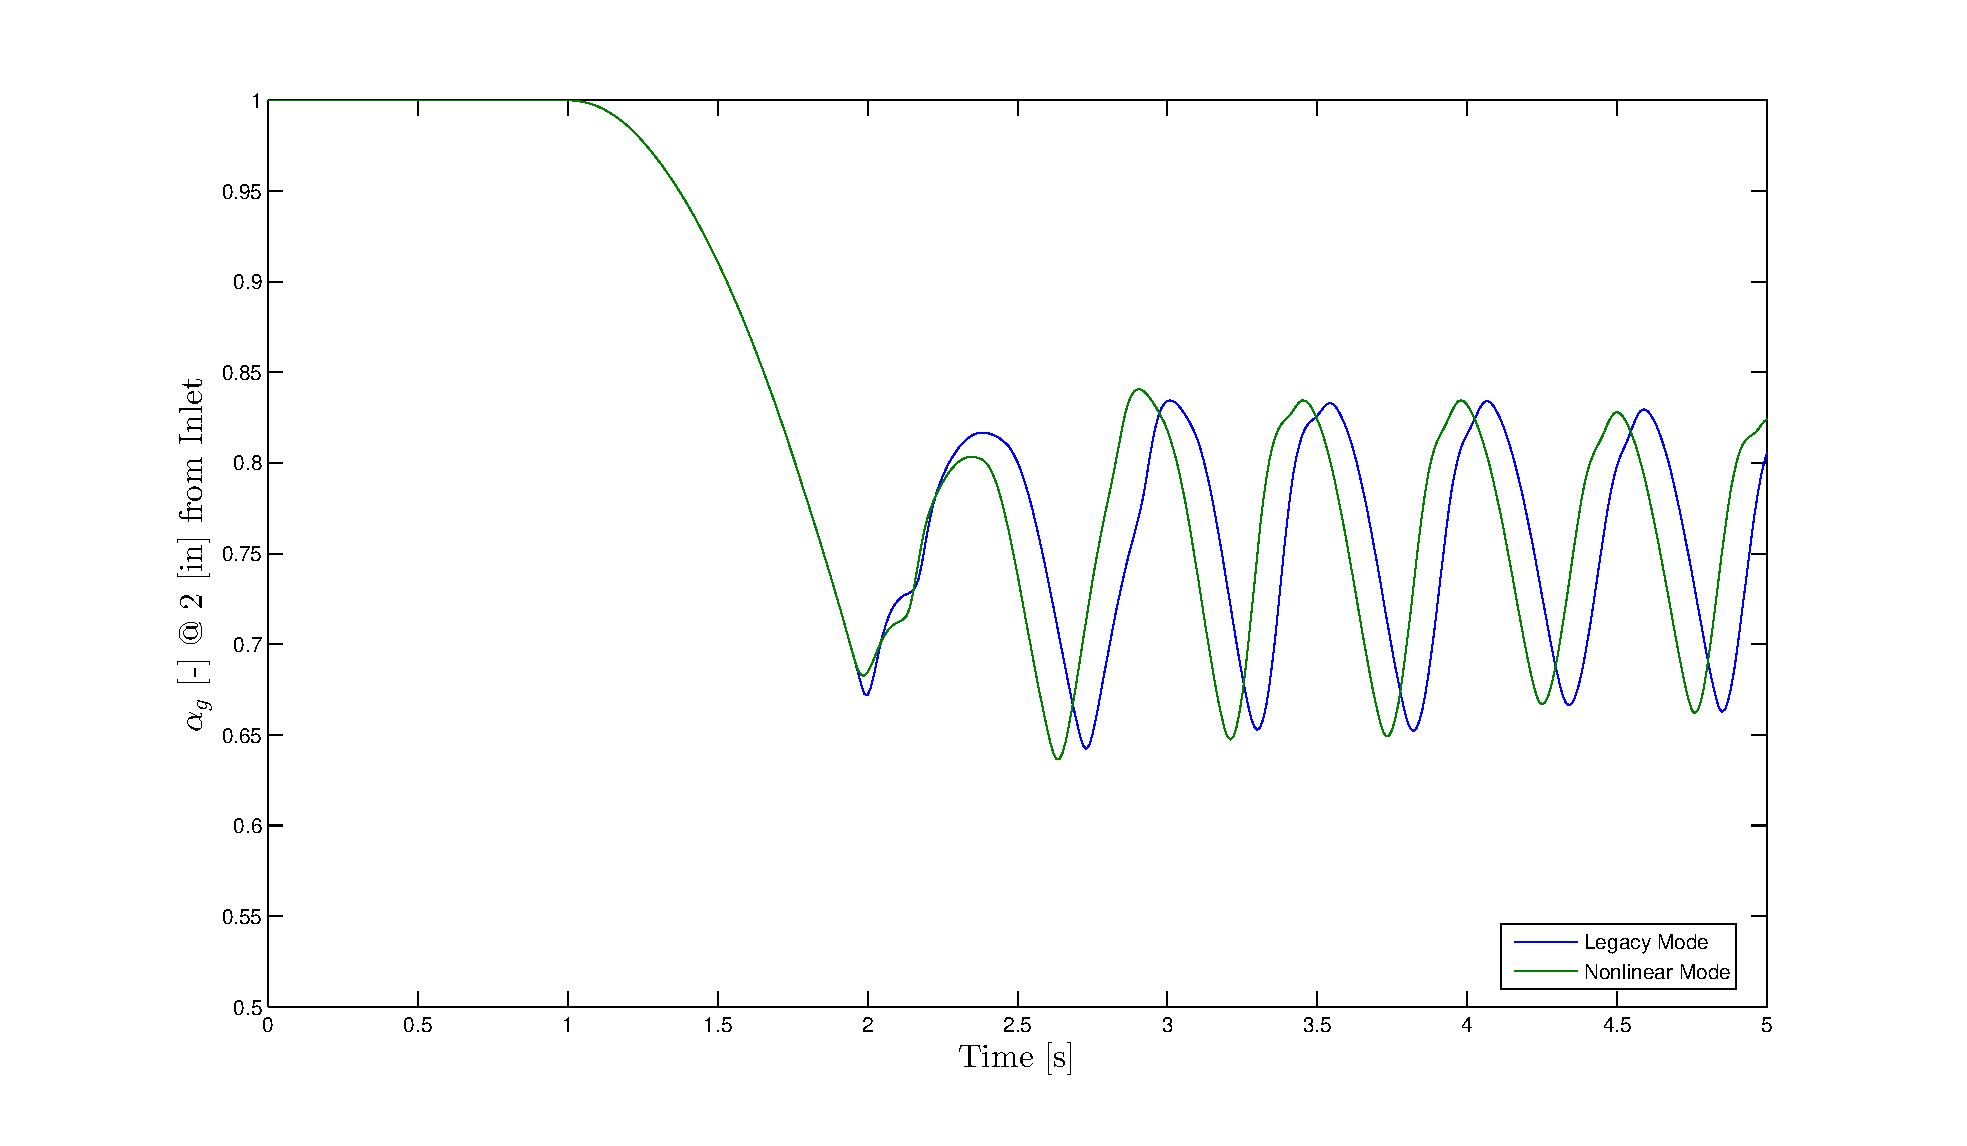
\includegraphics[width=0.49\textwidth]{images/flashing_1em5.eps}
%\label{fig:flashing_1em5}}
%\caption[Flashing solution at \dtmax{} = 1.0E-1 {[s]}and 1.0E-5 {[s]}]{Flashing solution at \dtmax{} = 1.0E-1 {[s]} and 1.0E-5 {[s]}.}
%\label{fig:flashing_compare_1}
%\end{figure}

\begin{figure}[h!t]
\centering
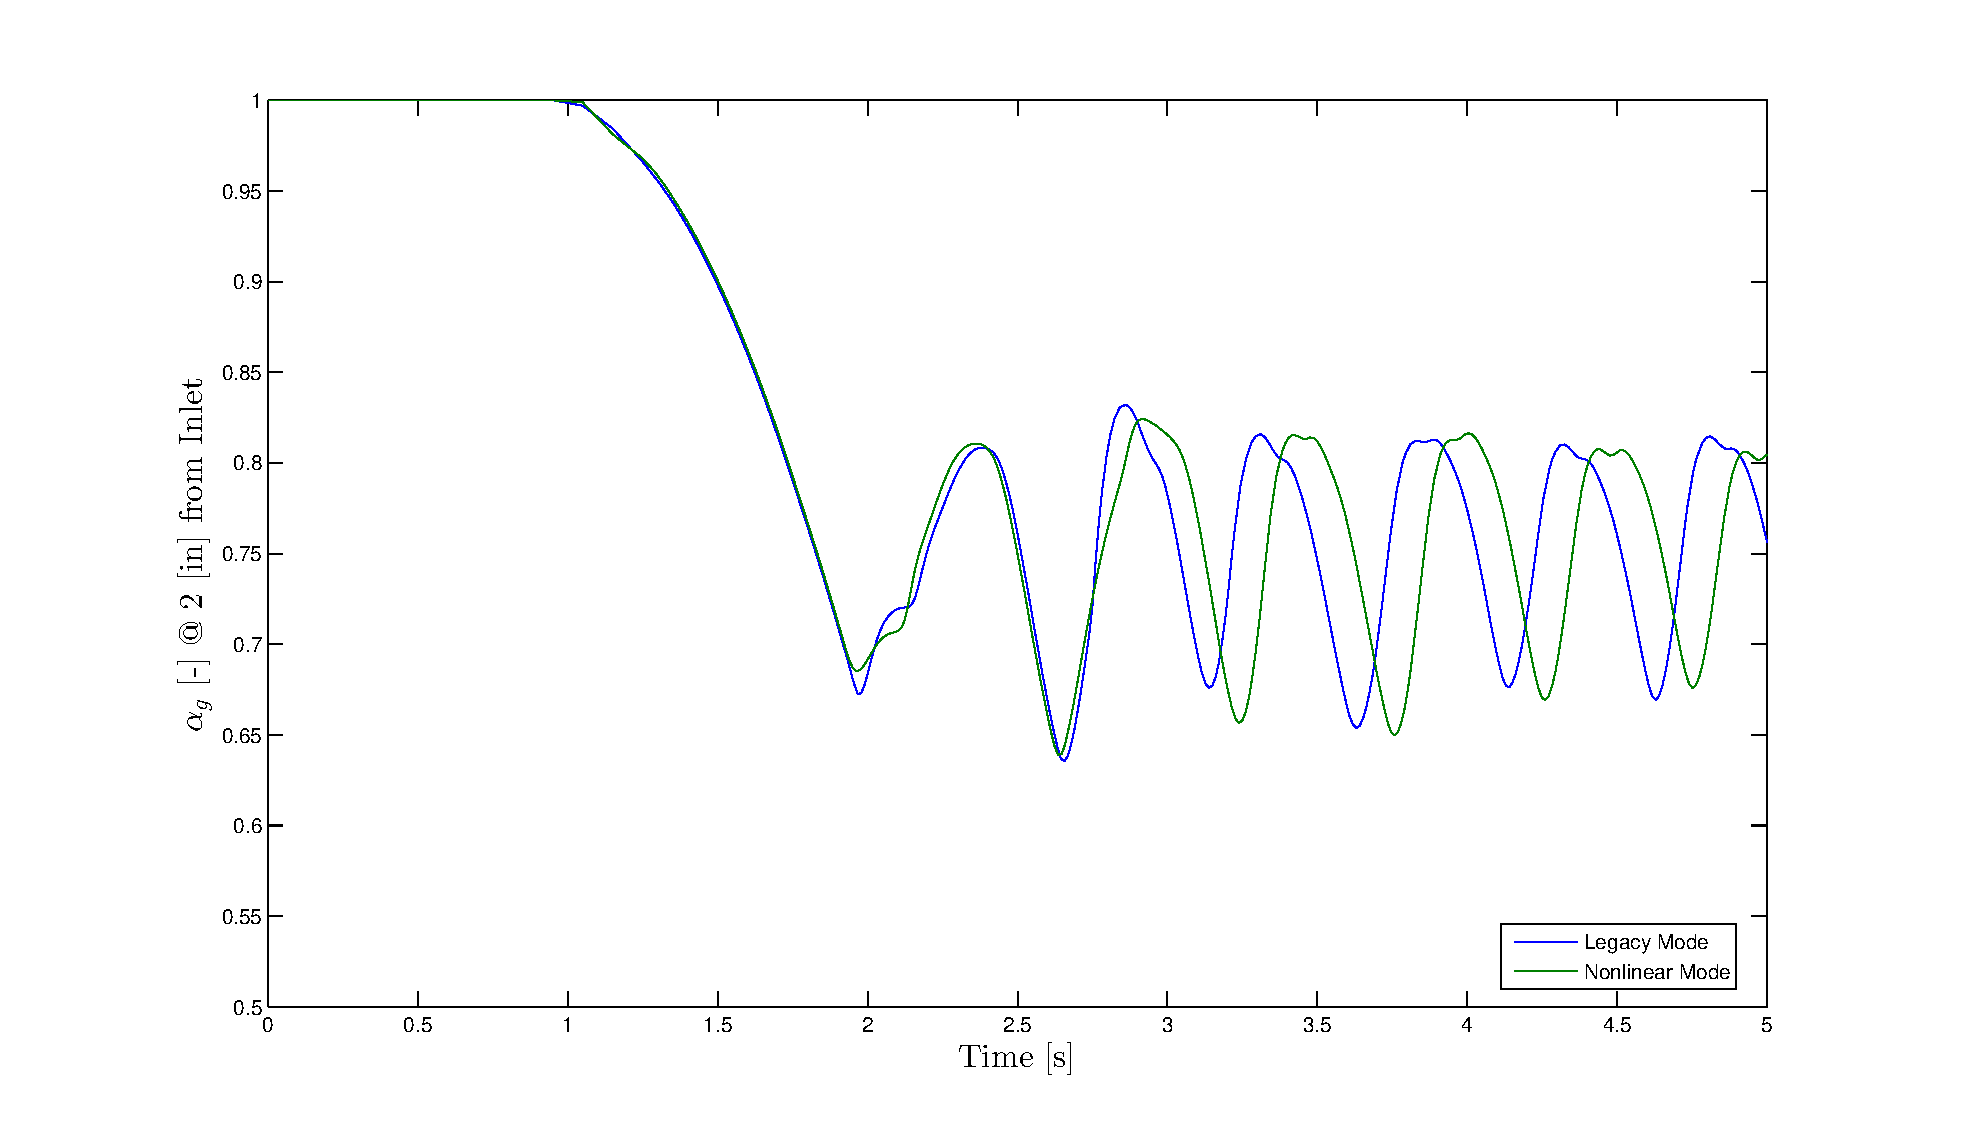
\includegraphics[width=0.94\textwidth]{images/flashing_1em1.eps}
\caption{Flashing solution at \dtmax{} = 1.0E-1 {[s]}}
\label{fig:flashing_1em1}
\end{figure}

\begin{figure}[h!t]
\centering
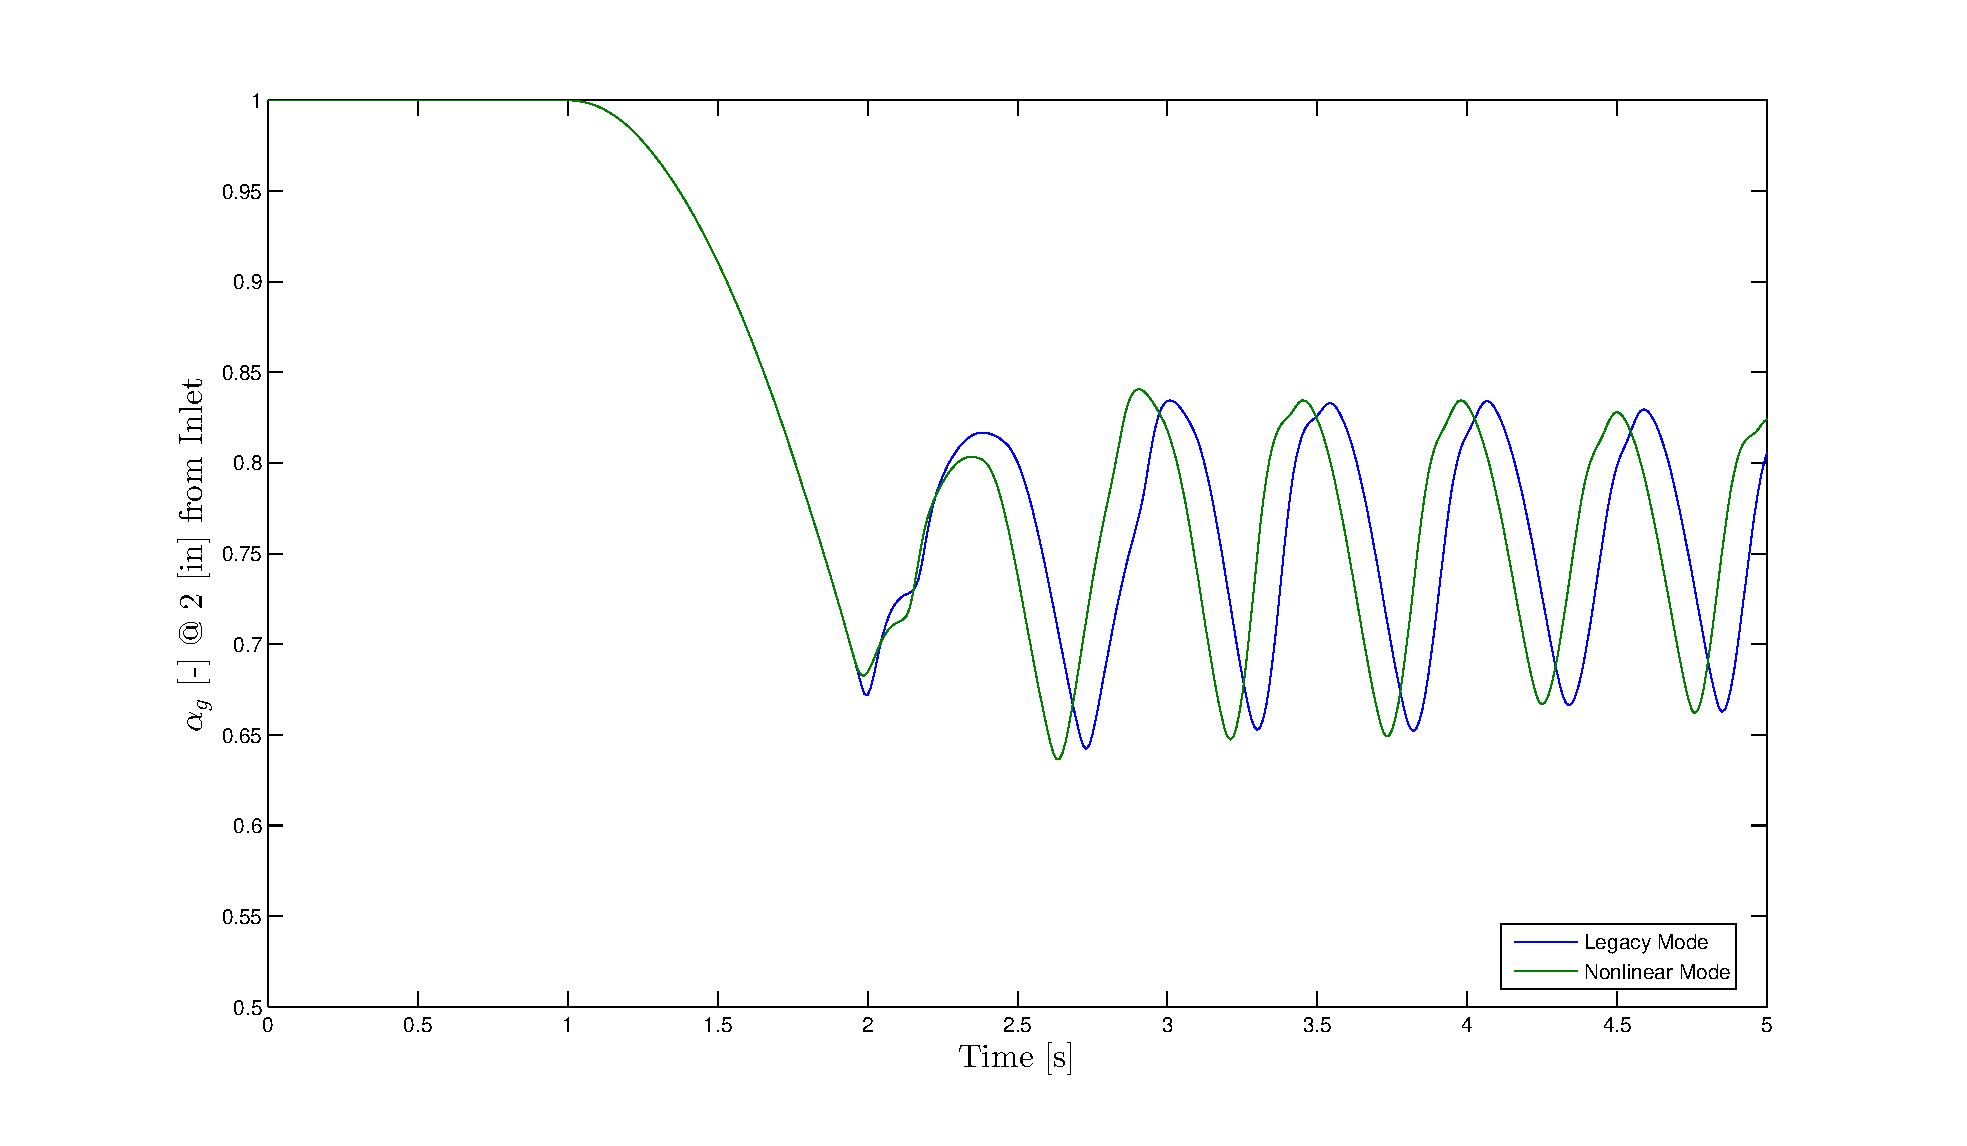
\includegraphics[width=.94\textwidth]{images/flashing_1em5.eps}
\caption{Flashing solution at \dtmax{} = 1.0E-5 {[s]}.}
\label{fig:flashing_1em5}
\end{figure}

Note that the nonlinearly resolved solution is qualitatively different than the legacy single-shot solution, \fig{fig:flashing_1em1}.
Even as the \dtmax{} is reduced, this discrepancy does not disappear, \fig{fig:flashing_1em5}.
The two solutions do not converge to the same solution as the timestep size was reduced.
However, the solution to the flashing problem produced by the nonlinear solver, \fig{fig:nl_mode_flashing}, qualitatively varies less as the timestep size is reduced than that produced by the legacy solver, \fig{fig:cobra_mode_flashing}.
However, both \fig{fig:cobra_mode_flashing} and \fig{fig:nl_mode_flashing} show that as the timestep size is reduced the two different solutions become more timestep size insensitive.

%\begin{figure}[h!t]
%\centering
%\subfloat[Legacy mode solution.]{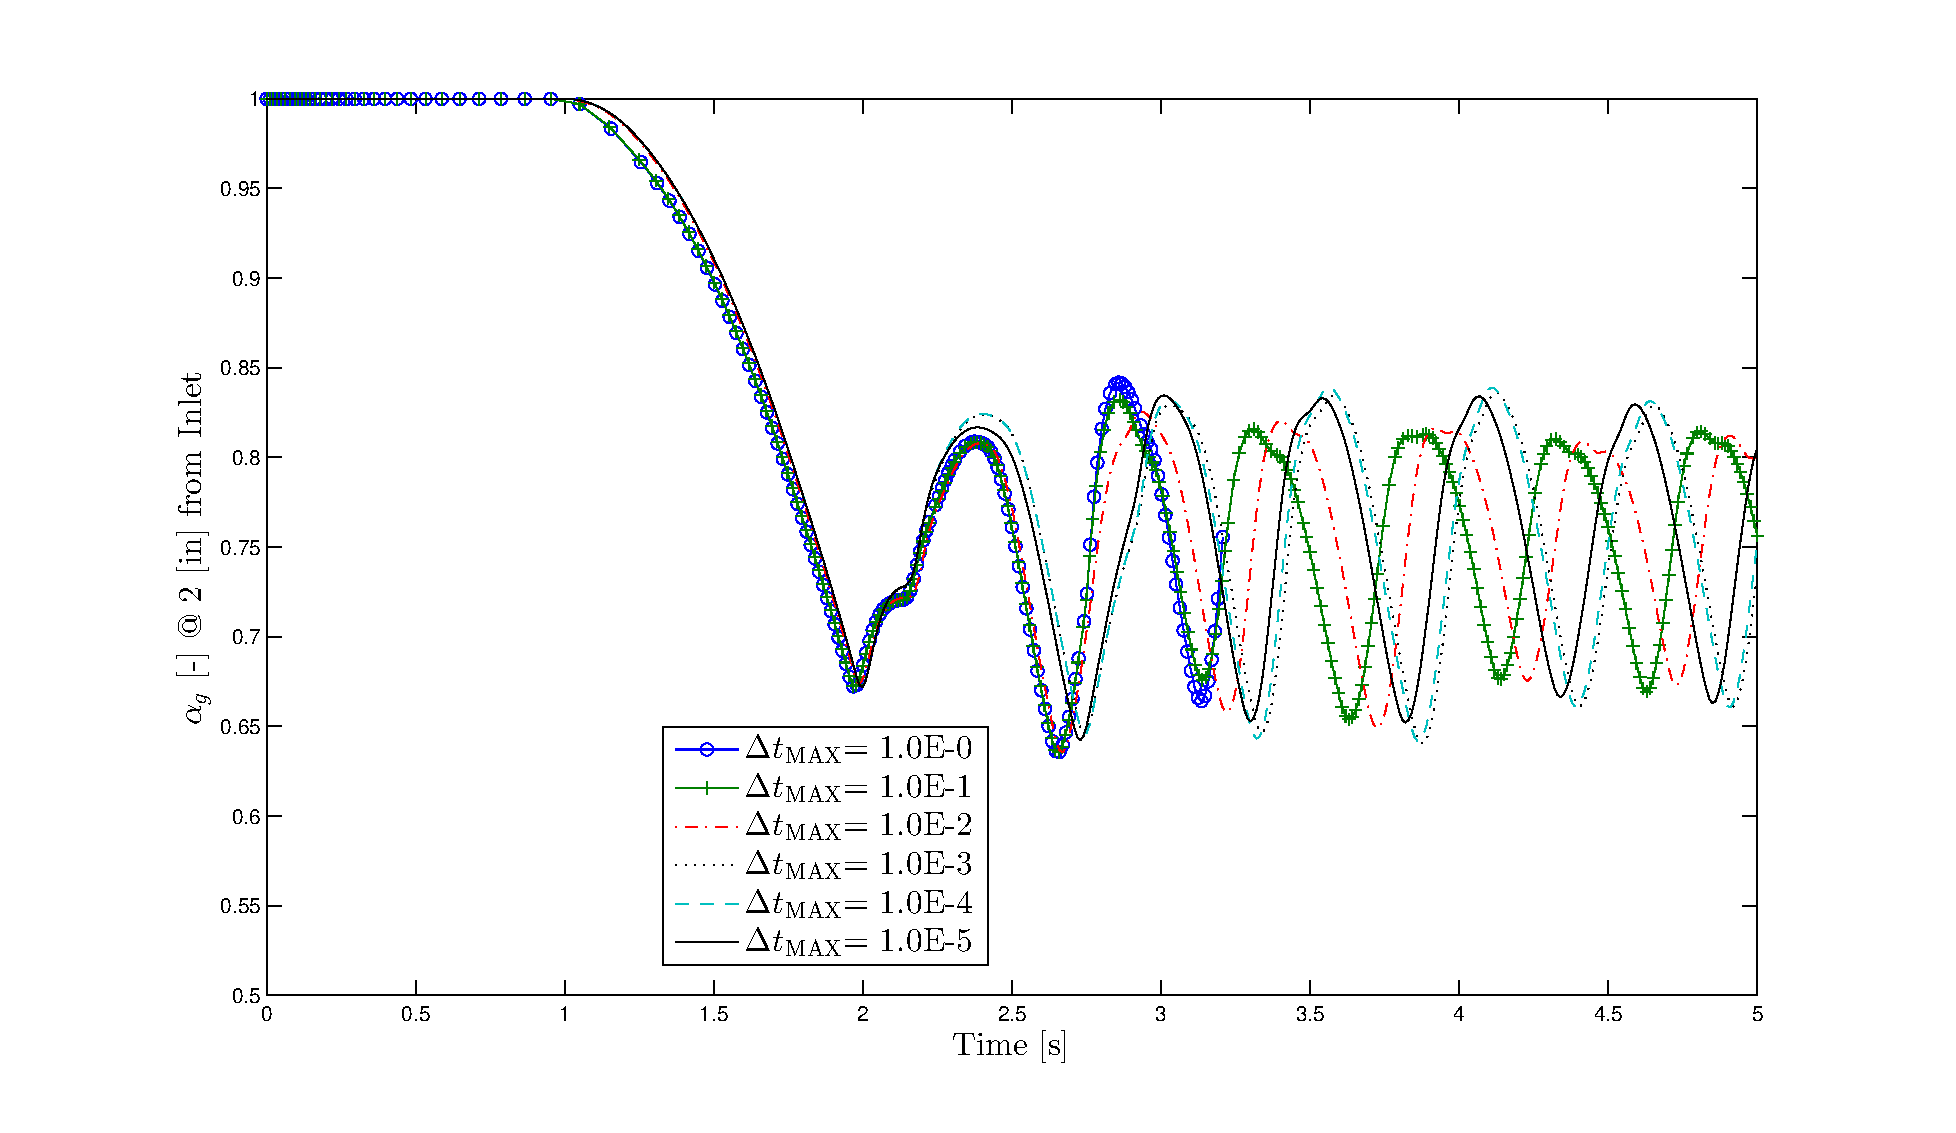
\includegraphics[width=0.49\textwidth]{images/cobra_flashing_al_2in.eps}
%\label{fig:cobra_mode_flashing}}
%\subfloat[Nonlinear mode solution.]{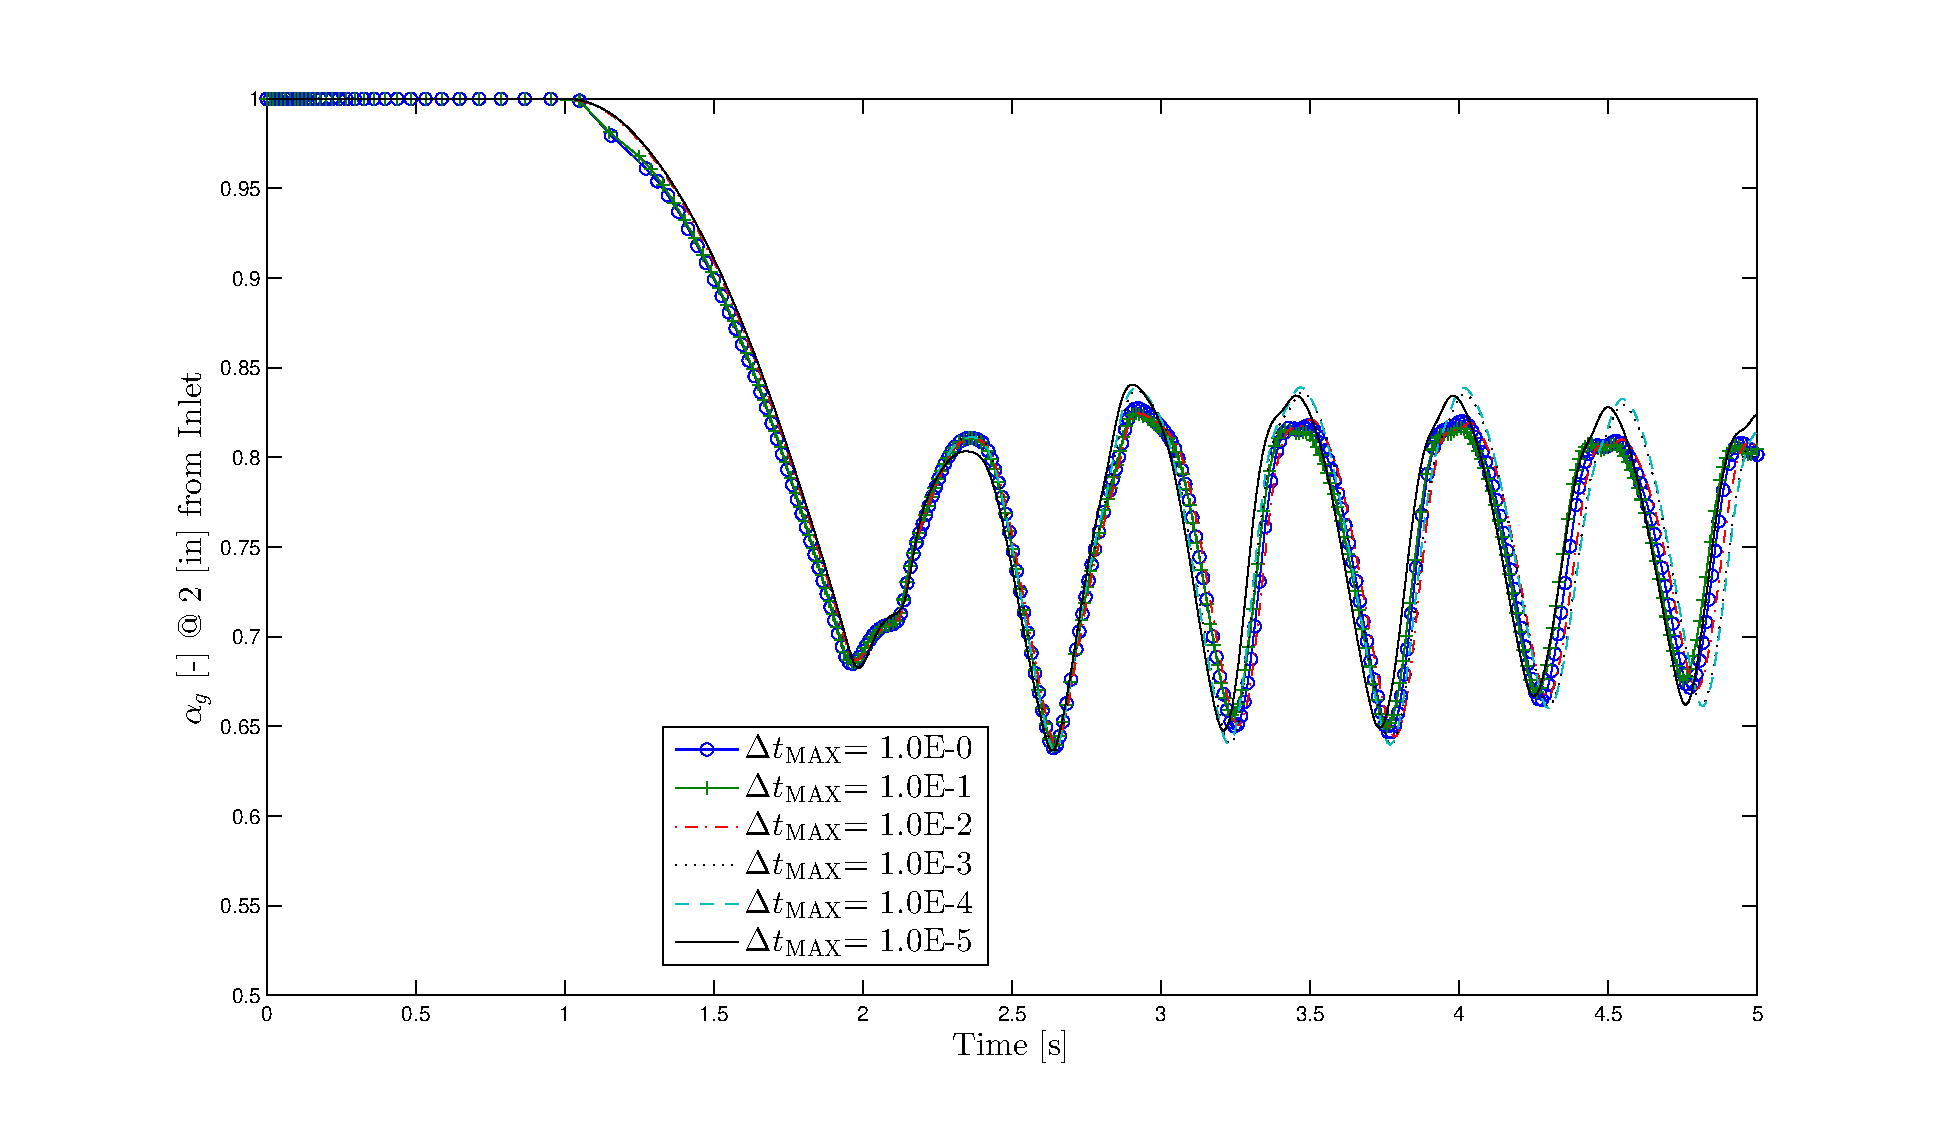
\includegraphics[width=0.49\textwidth]{images/nl_flashing_al_2in.eps}
%\label{fig:nl_mode_flashing}}
%\caption{Flashing simulation.}
%\label{fig:flashing_solutions_1}
%\end{figure}

\begin{figure}[h!t]
\centering
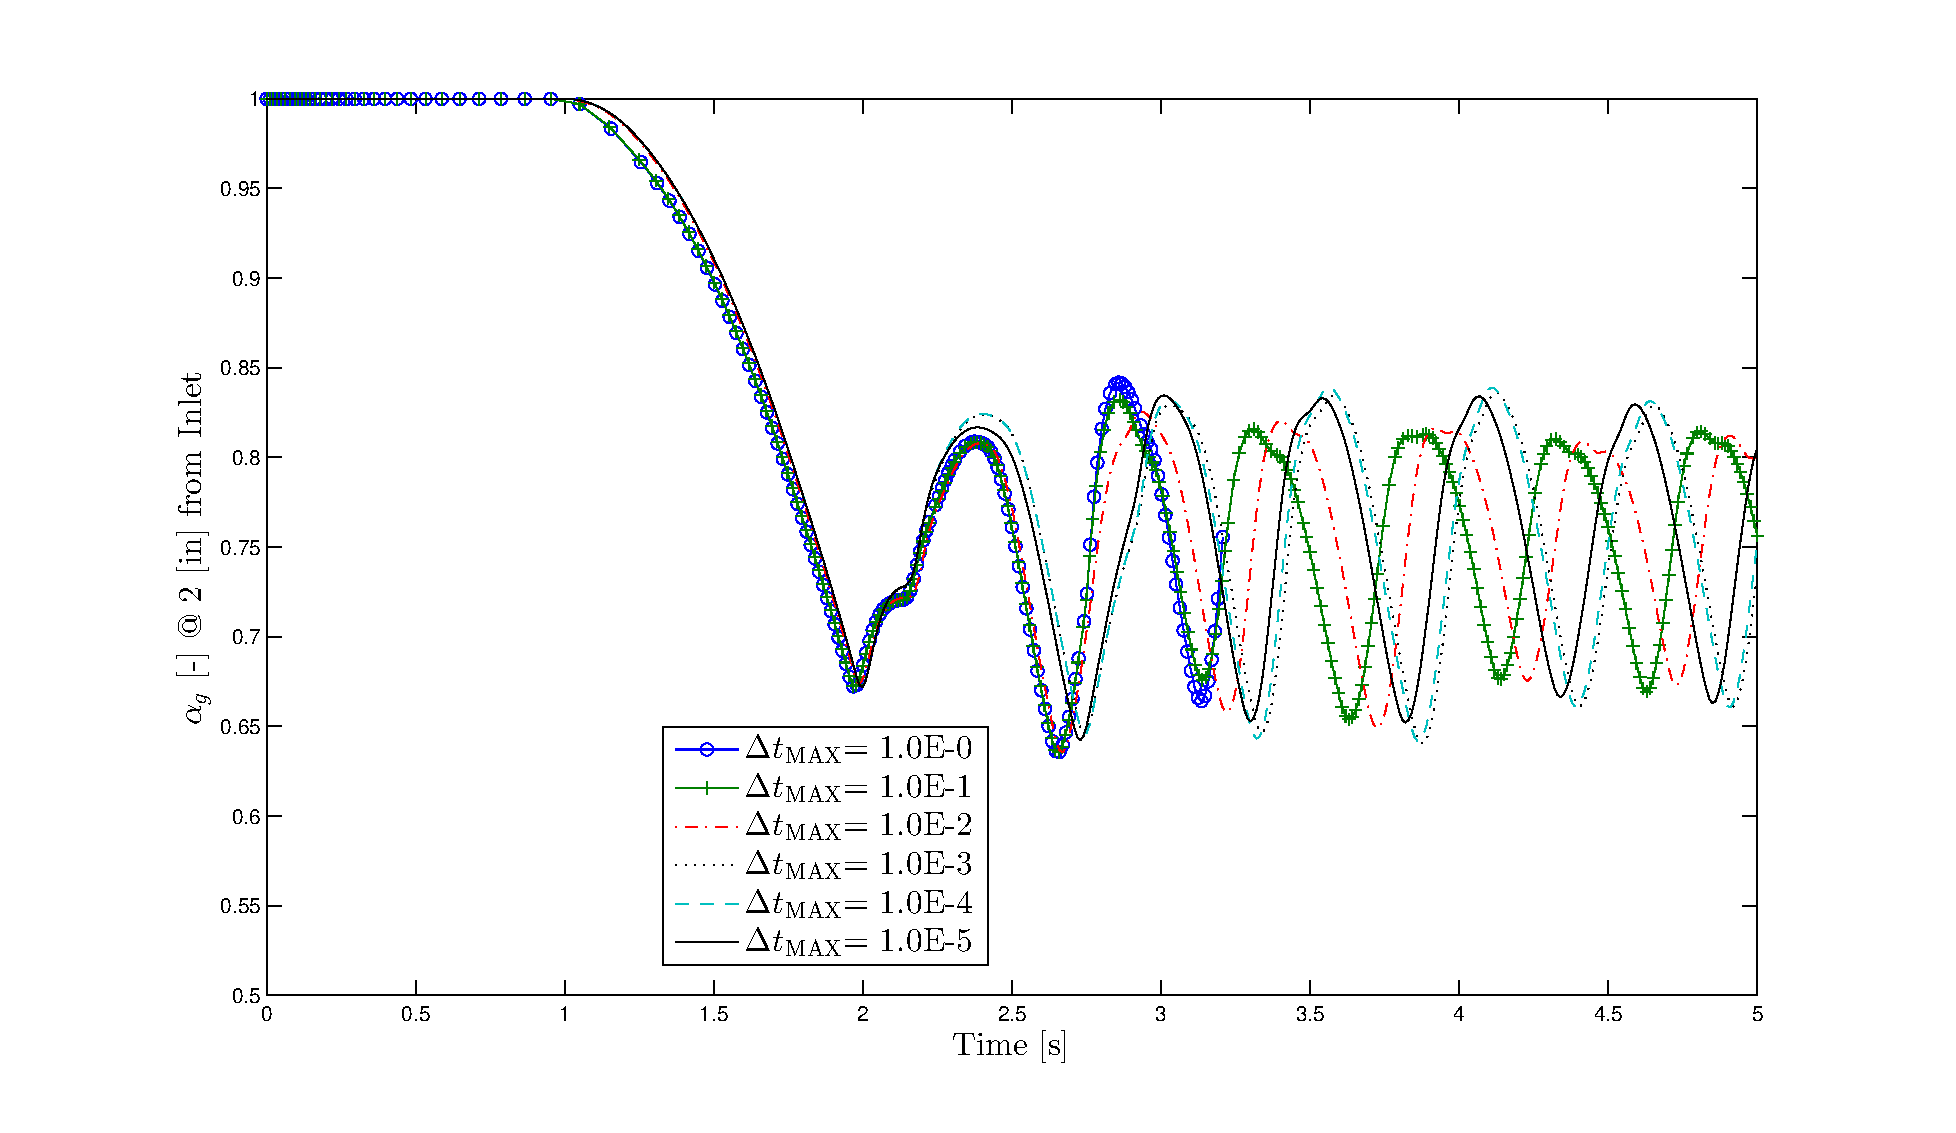
\includegraphics[width=.94\textwidth]{images/cobra_flashing_al_2in.eps}
\caption{Legacy solver flashing solution.}
\label{fig:cobra_mode_flashing}
\end{figure}

\begin{figure}[h!t]
\centering
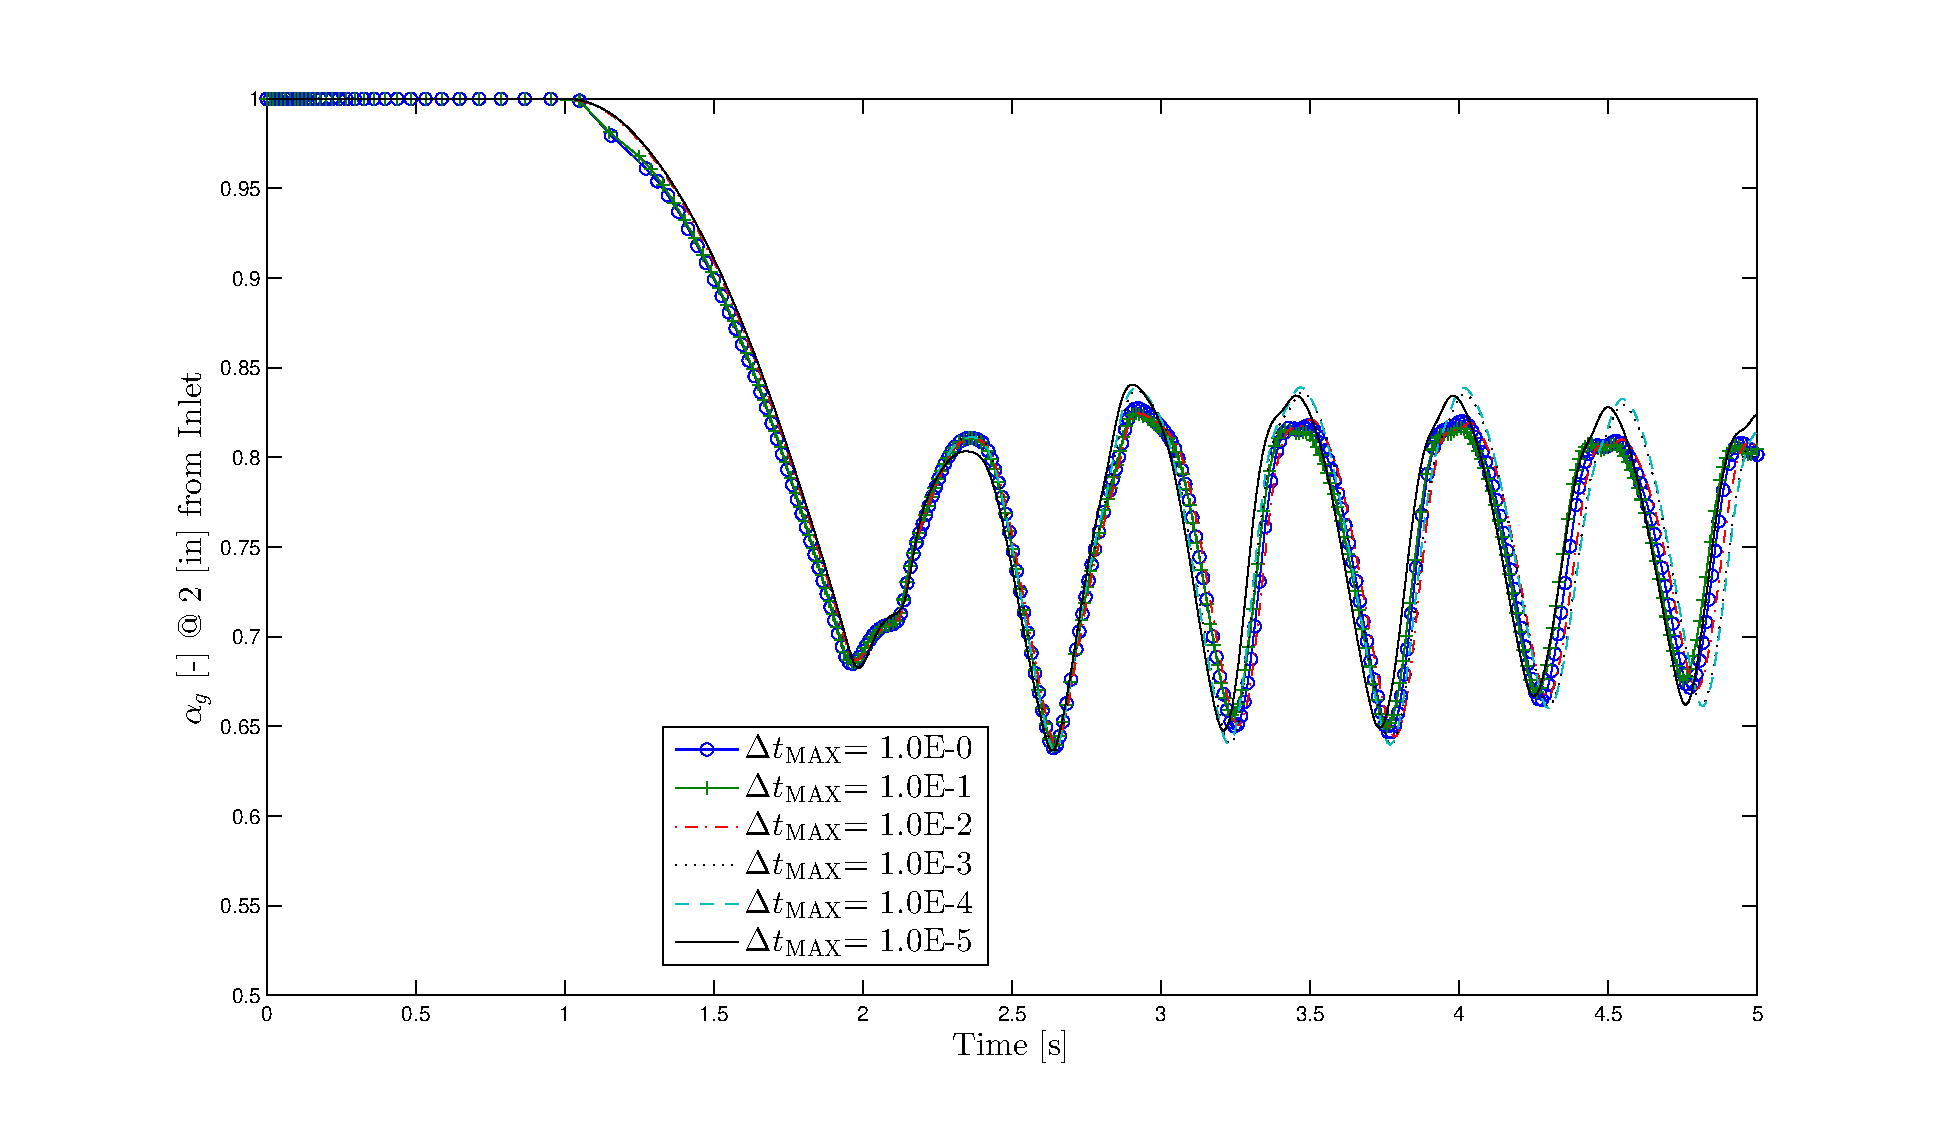
\includegraphics[width=.94\textwidth]{images/nl_flashing_al_2in.eps}
\caption{Nonlinear solver flashing solution.}
\label{fig:nl_mode_flashing}
\end{figure}

The two solvers, when applied to the same problem that contains highly nonlinear physics, produce two different timestep size invariant solutions.
These two solutions achieve qualitative timestep size invariance at different timestep sizes.
The parameter of interest in the solution produced by the nonlinear solver with a 1 [s] $\Delta t_{\text{MAX}}$ is qualitatively close to that produced with a 0.1 [s] $\Delta t_{\text{MAX}}$, \fig{fig:nl_flashing_compare}.
The same level of qualitative timestep size invariance is achieved in the legacy solver solutions between a \dtmax{} of 1.0E-3 [s] and 1.0E-4 [s], \fig{fig:cobra_flashing_compare}.

%\begin{figure}[h!t]
%\centering
%\subfloat[Nonlinear mode solution.]{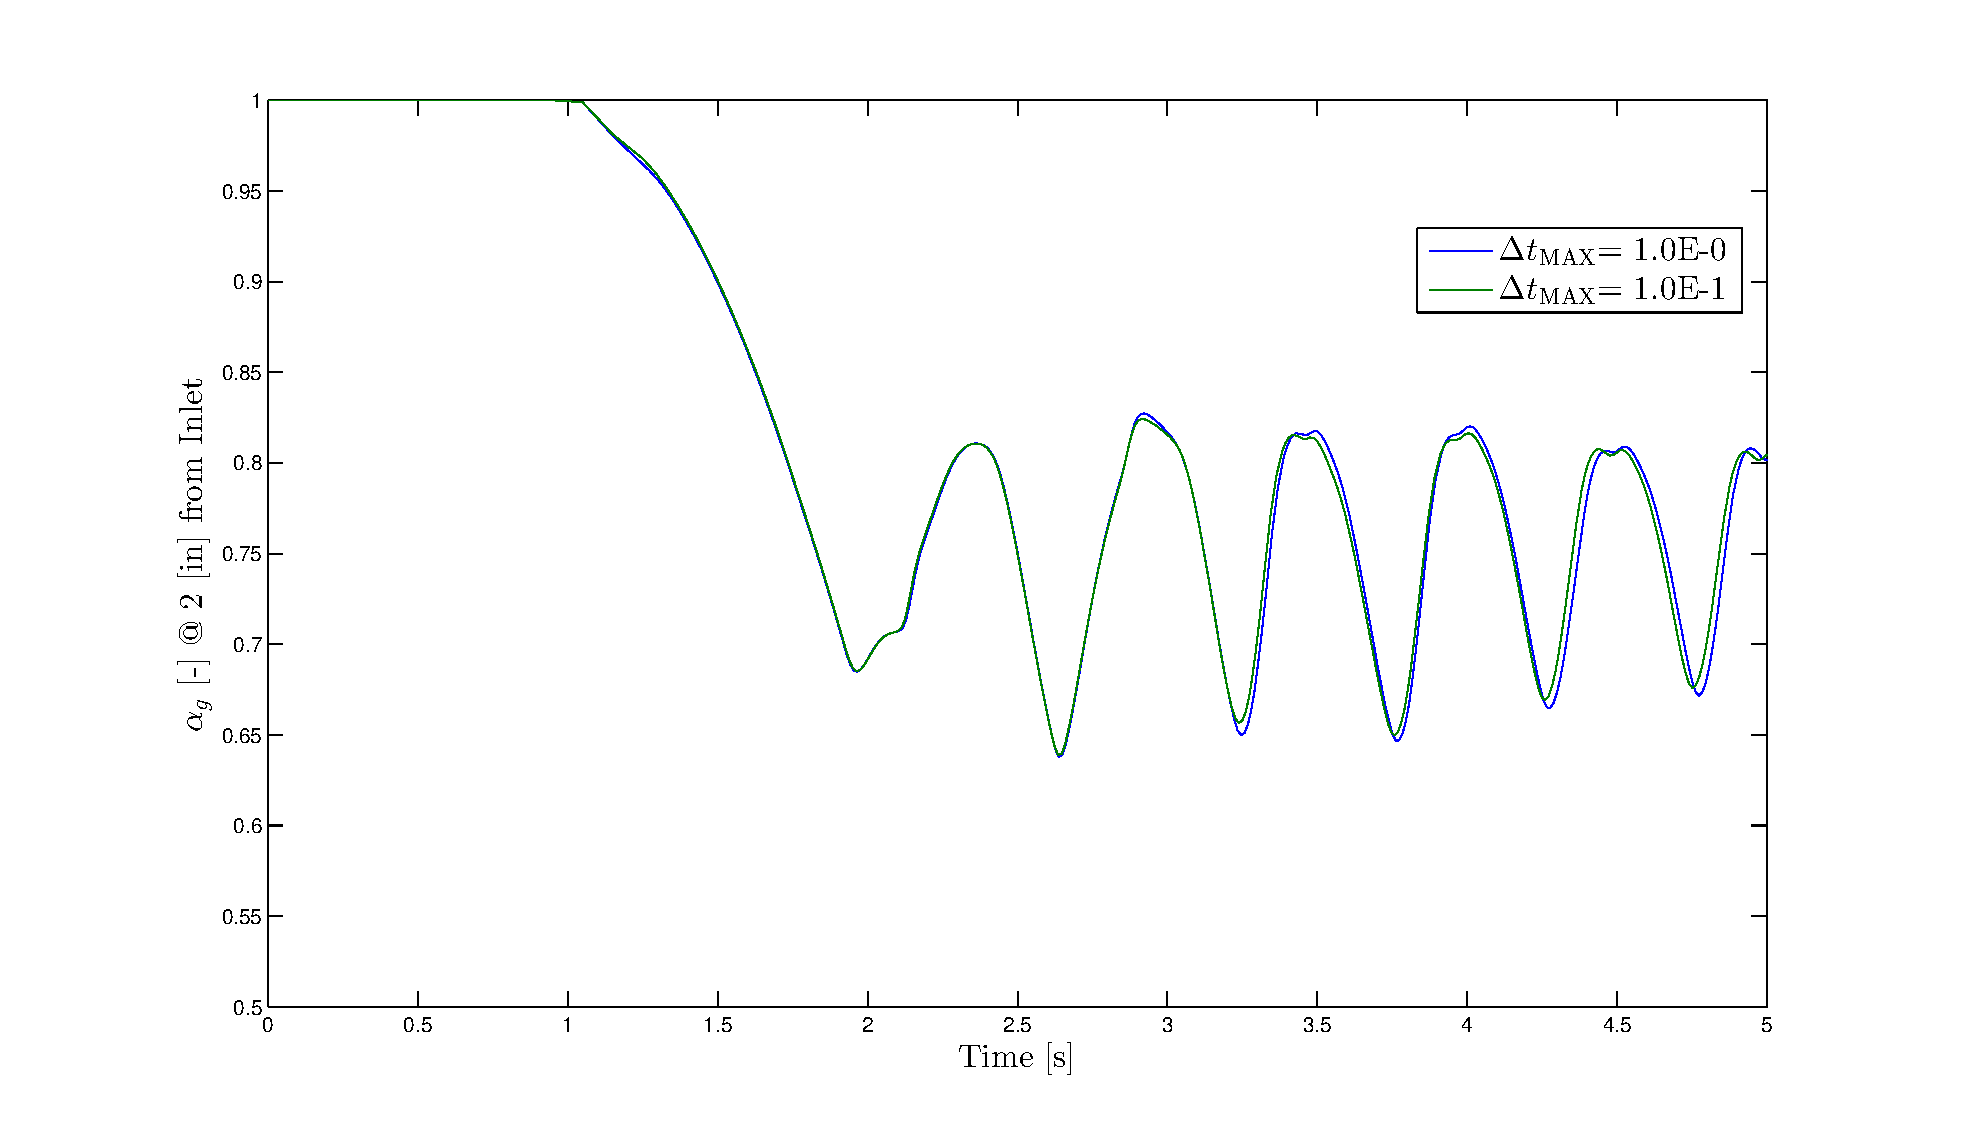
\includegraphics[width=0.49\textwidth]{images/nl_flashing_1em0_1em1.eps}
%\label{fig:nl_flashing_compare}}
%\subfloat[Legacy mode solution.]{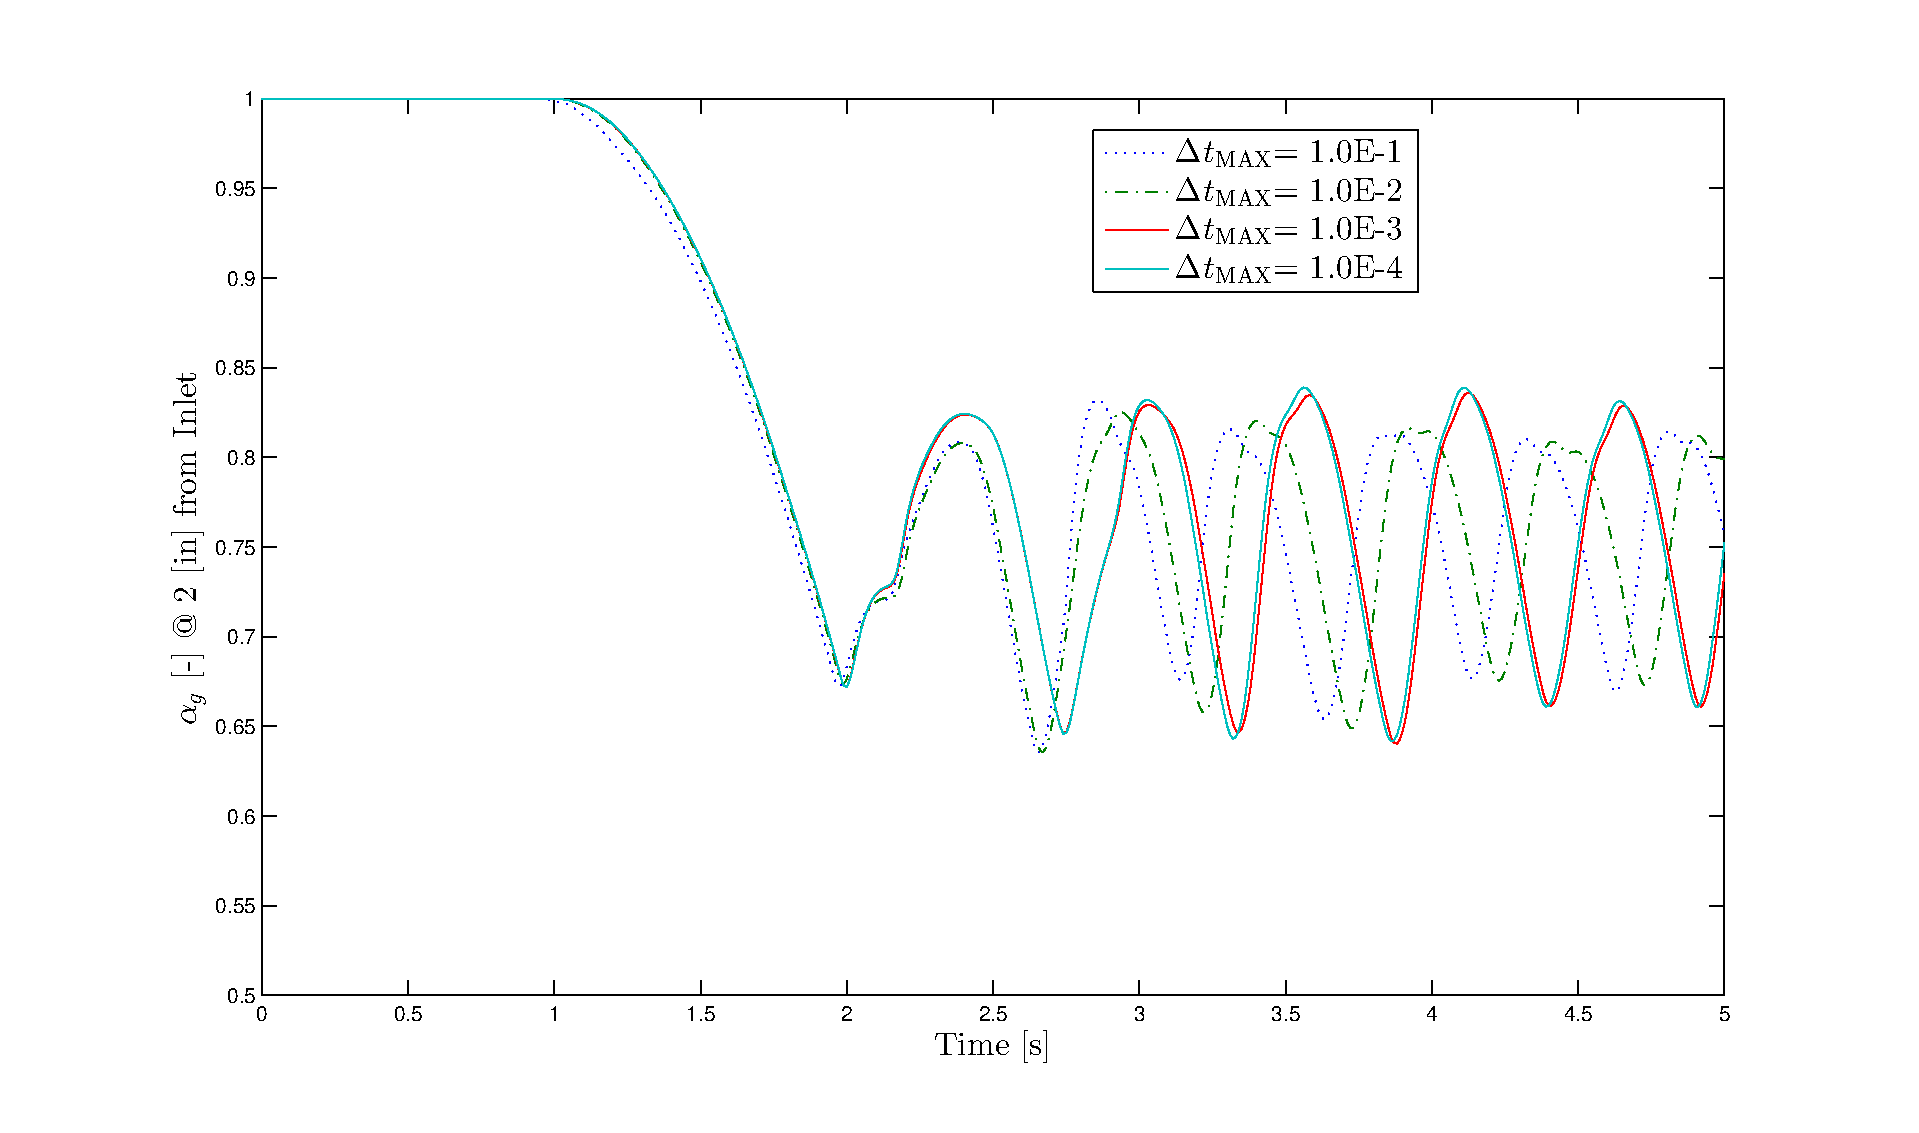
\includegraphics[width=0.49\textwidth]{images/cobra_flashing_1em1_1em4.eps}
%\label{fig:cobra_flashing_compare}}
%\caption{Timestep size insensitive flashing solutions.}
%\label{fig:flashing_res_comp_1}
%\end{figure}

\begin{figure}[h!t]
\centering
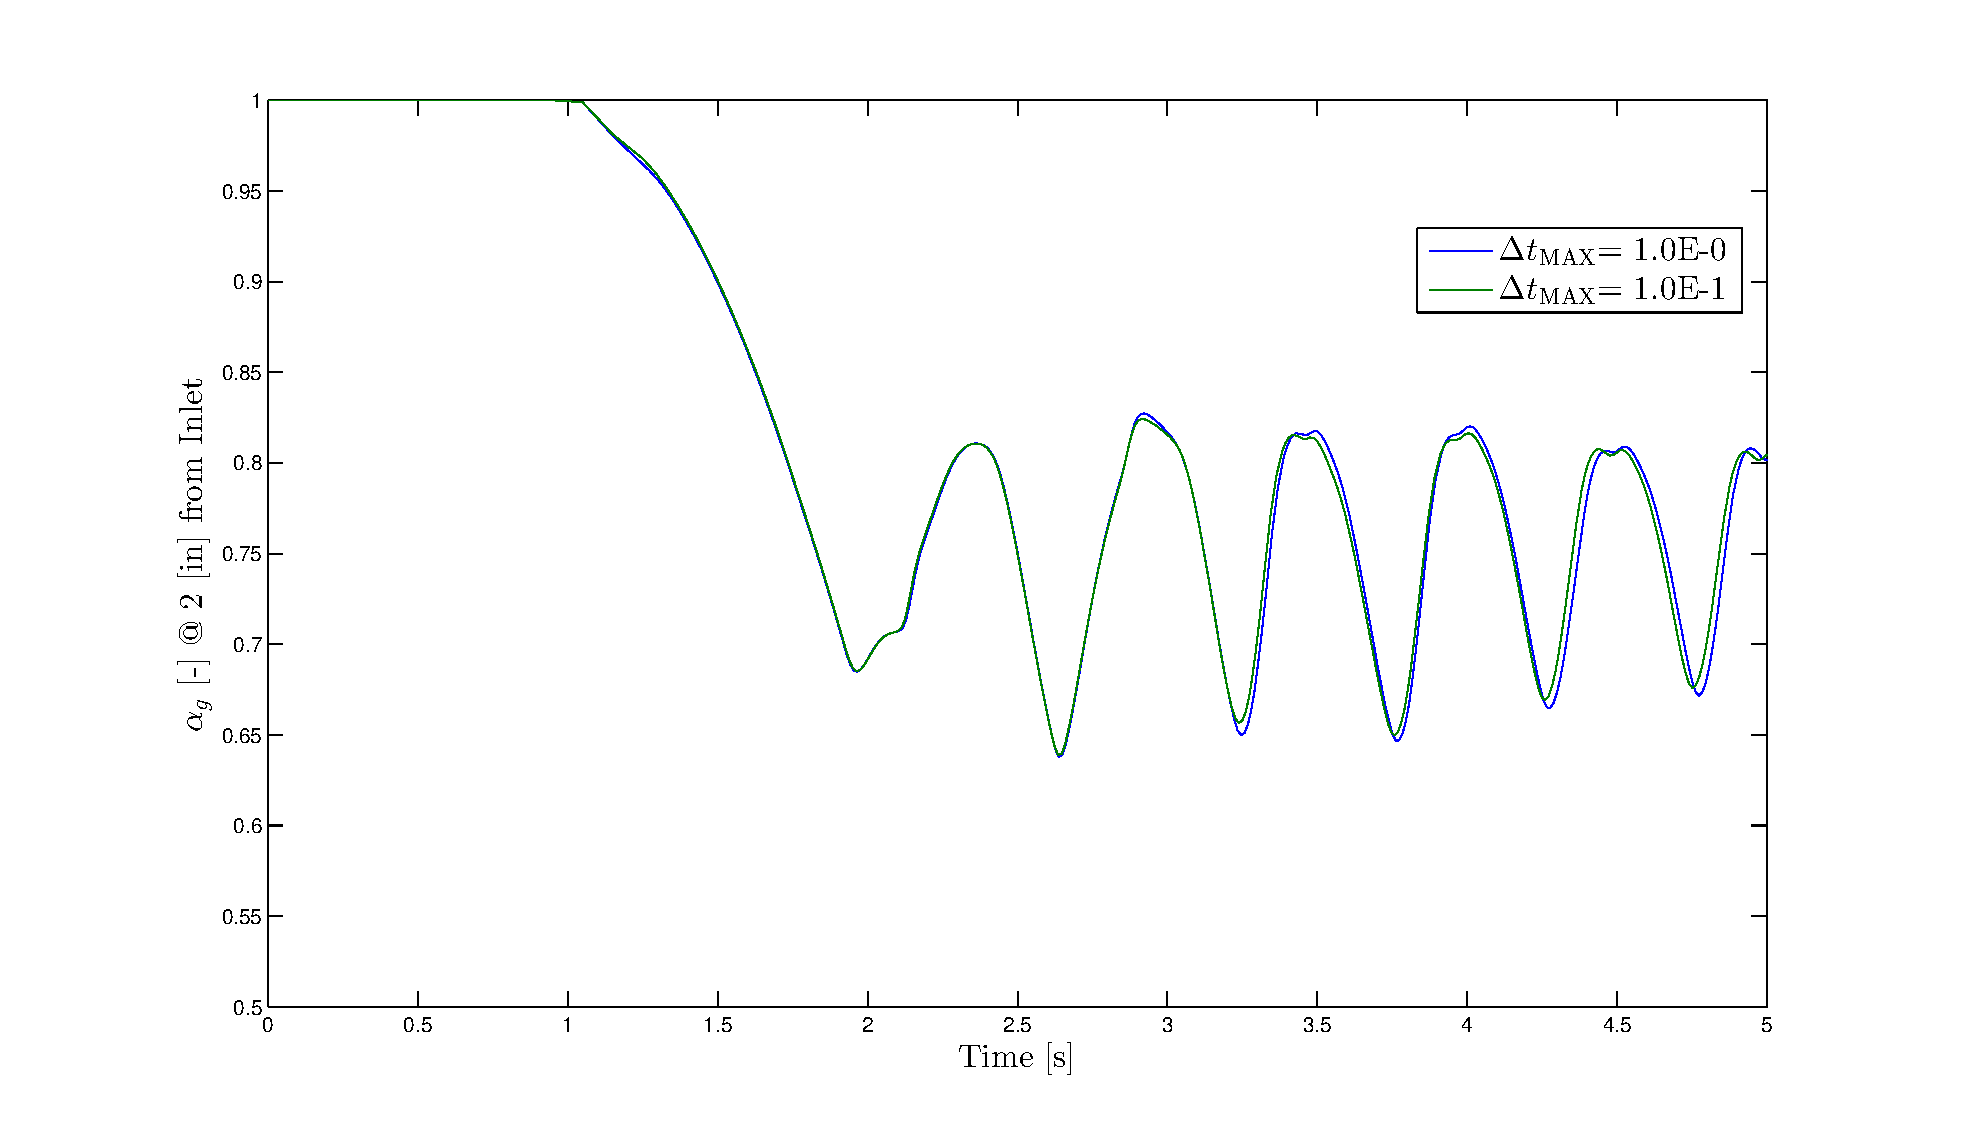
\includegraphics[width=.94\textwidth]{images/nl_flashing_1em0_1em1.eps}
\caption{Nonlinear solver timestep size insensitive flashing solution.}
\label{fig:nl_flashing_compare}
\end{figure}

\begin{figure}[h!t]
\centering
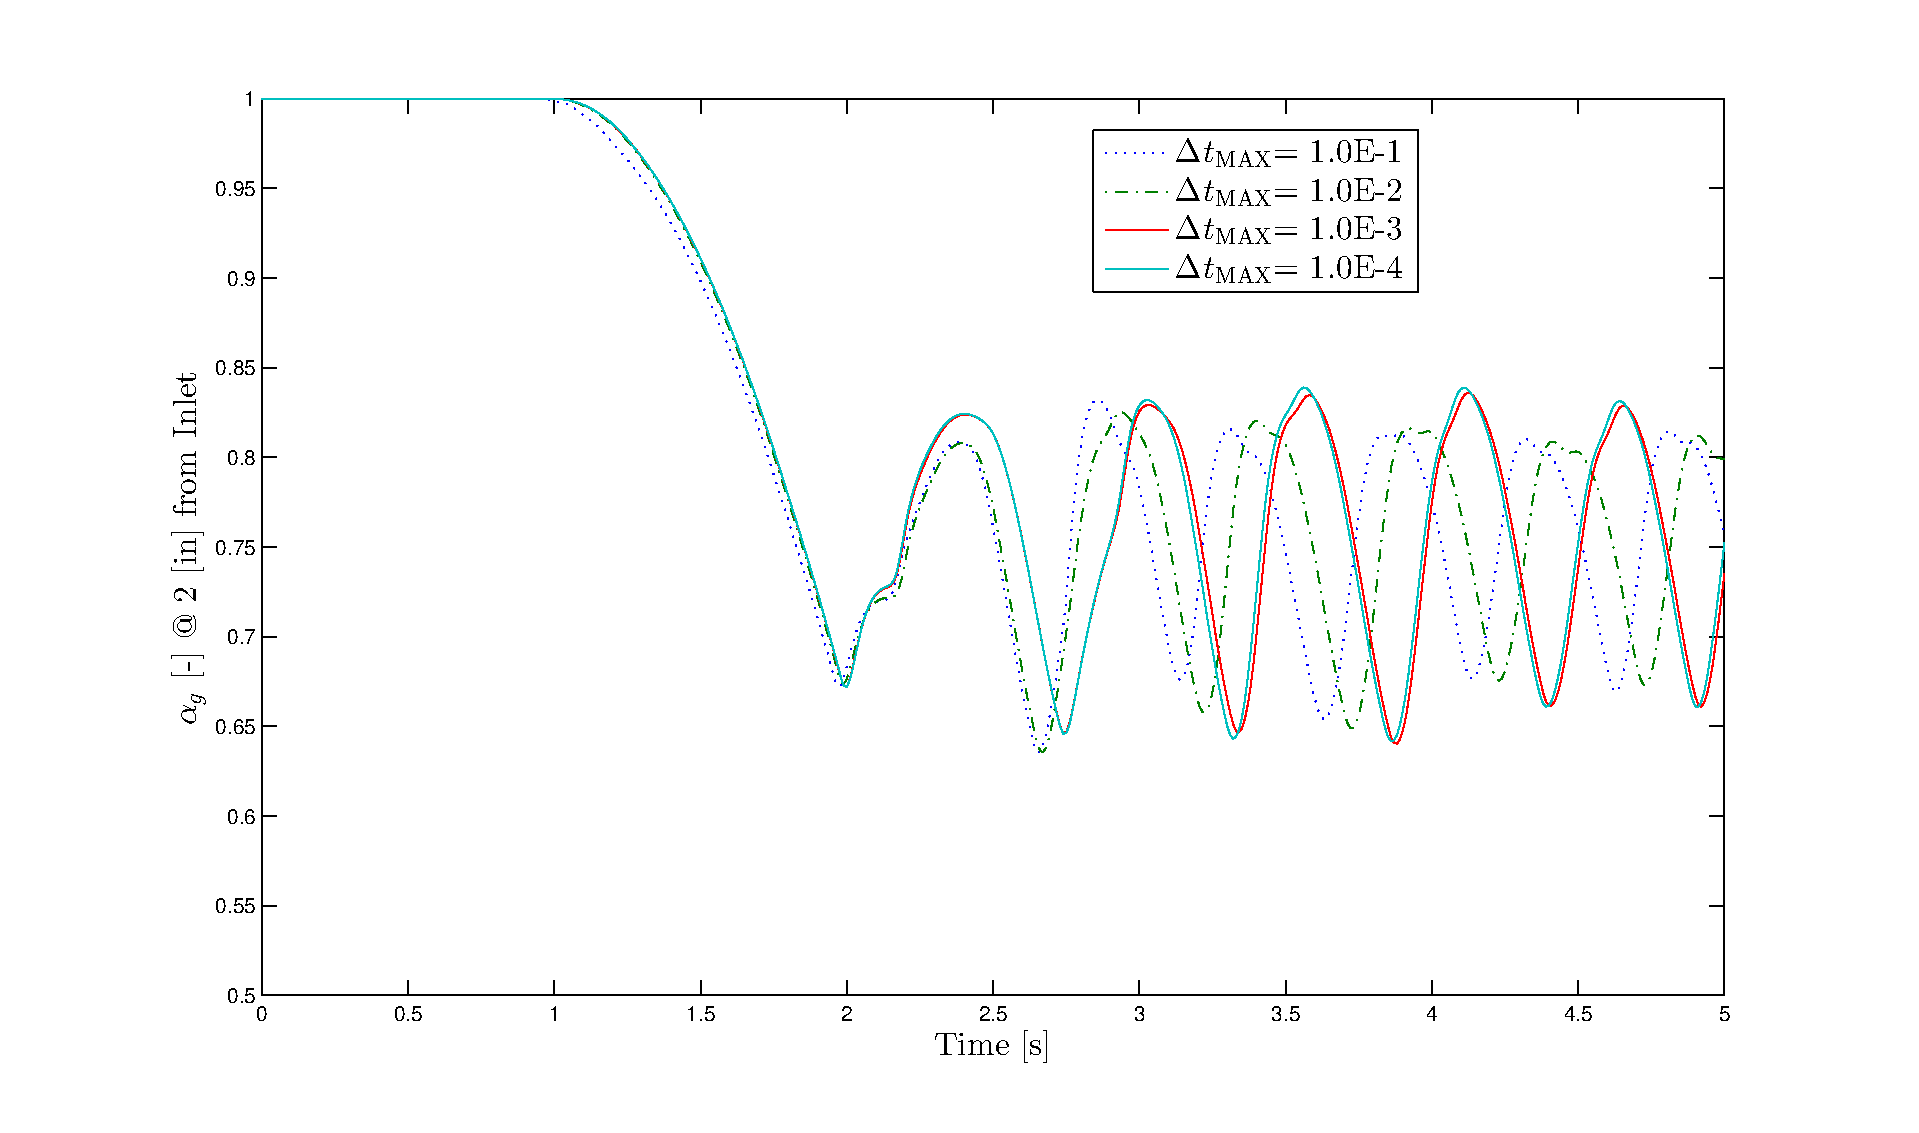
\includegraphics[width=.94\textwidth]{images/cobra_flashing_1em1_1em4.eps}
\caption{Legacy solver timestep size insensitive flashing solution.}
\label{fig:cobra_flashing_compare}
\end{figure}

The timestep size insensitive solution produced by the nonlinear solver occurs at a maximum timestep size three orders of magnitude greater than that achieved by the legacy solver in \cobra{}.
An examination of the nonlinear residual over the course of the transient provides insight into why this behavior is observed.
The scaled residual for the legacy flashing problem indicates that, even for small timestep sizes, the solution obtained still does not satisfy the discrete nonlinear equations, \fig{fig:legacy_flashing_residual}.
This is in contrast to the nonlinear flashing problem, which shows a lower residual over the course of the simulation, \fig{fig:nonlinear_flashing_residual}.

%\begin{figure}[h!t]
%\centering
%\subfloat[Legacy solver residuals.]{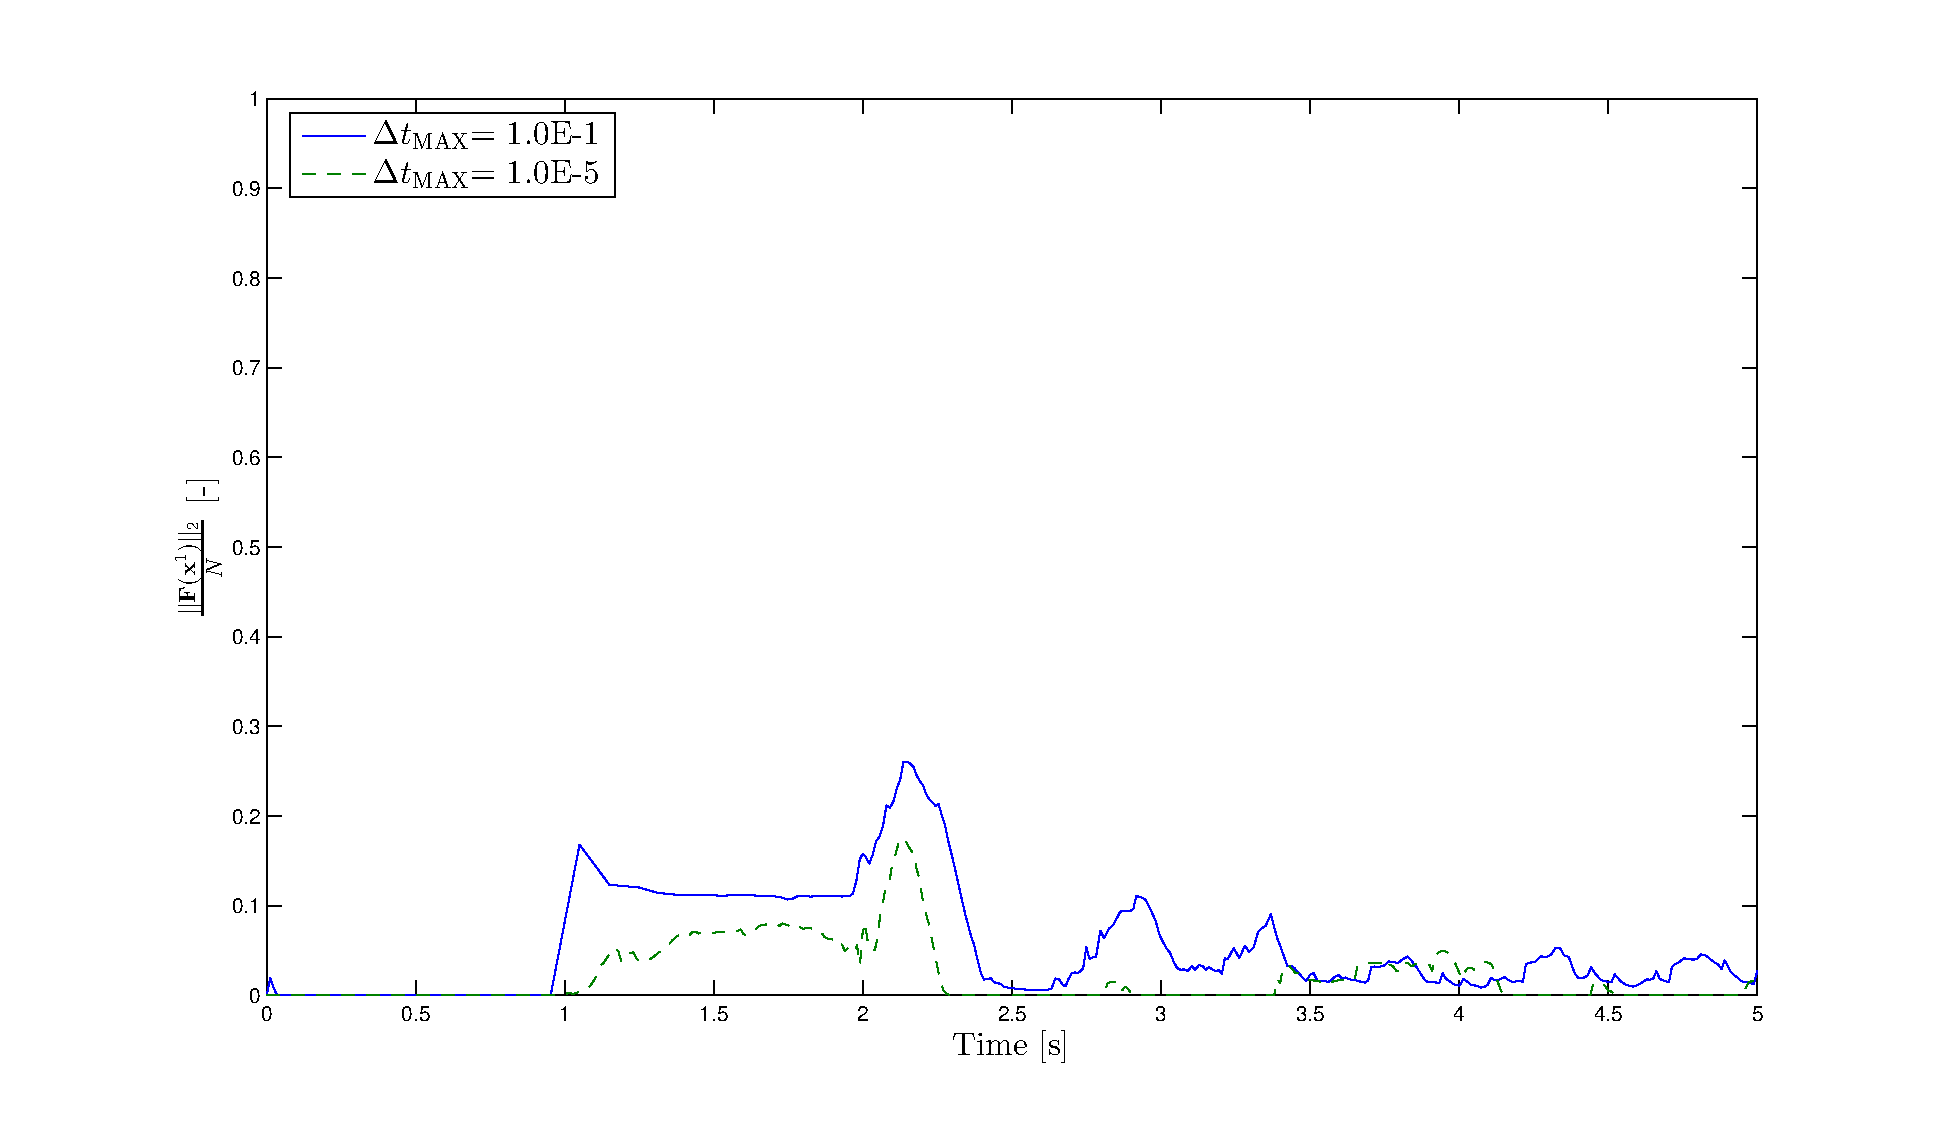
\includegraphics[width=0.49\textwidth]{images/cobra_flashing_res_compare.eps}
%\label{fig:legacy_flashing_residual}}
%\subfloat[Nonlinear solver residuals.]{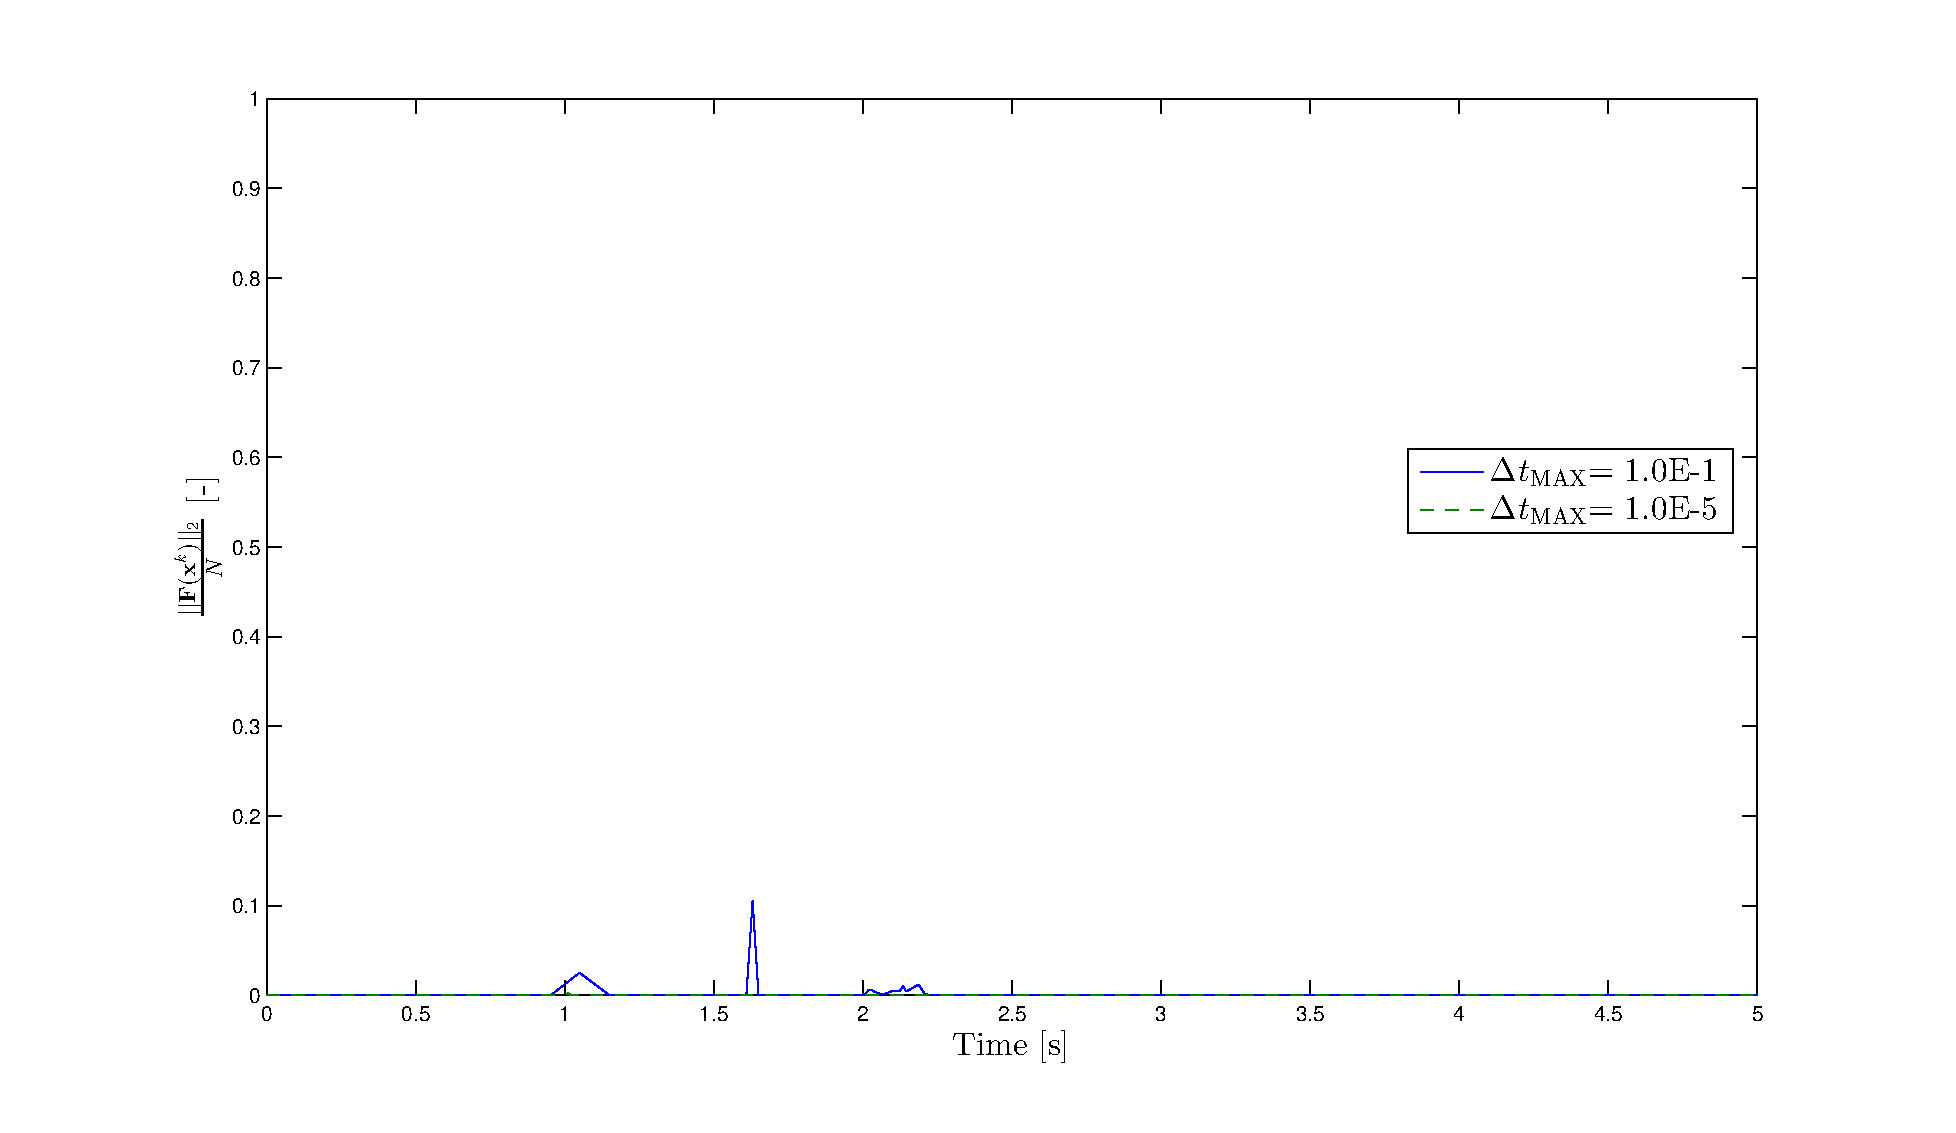
\includegraphics[width=0.49\textwidth]{images/nl_flashing_res_compare.eps}
%\label{fig:nonlinear_flashing_residual}}
%\caption[Flashing residual at $\Delta t_{\text{MAX}}$ = 1.0E-1 {[s]}and 1.0E-5 {[s]}]{Flashing residual at $\Delta t_{\text{MAX}}$ = 1.0E-1 {[s]} and 1.0E-5 {[s]}.}
%\label{fig:flashing_compare_2}
%\end{figure}

\begin{figure}[h!t]
\centering
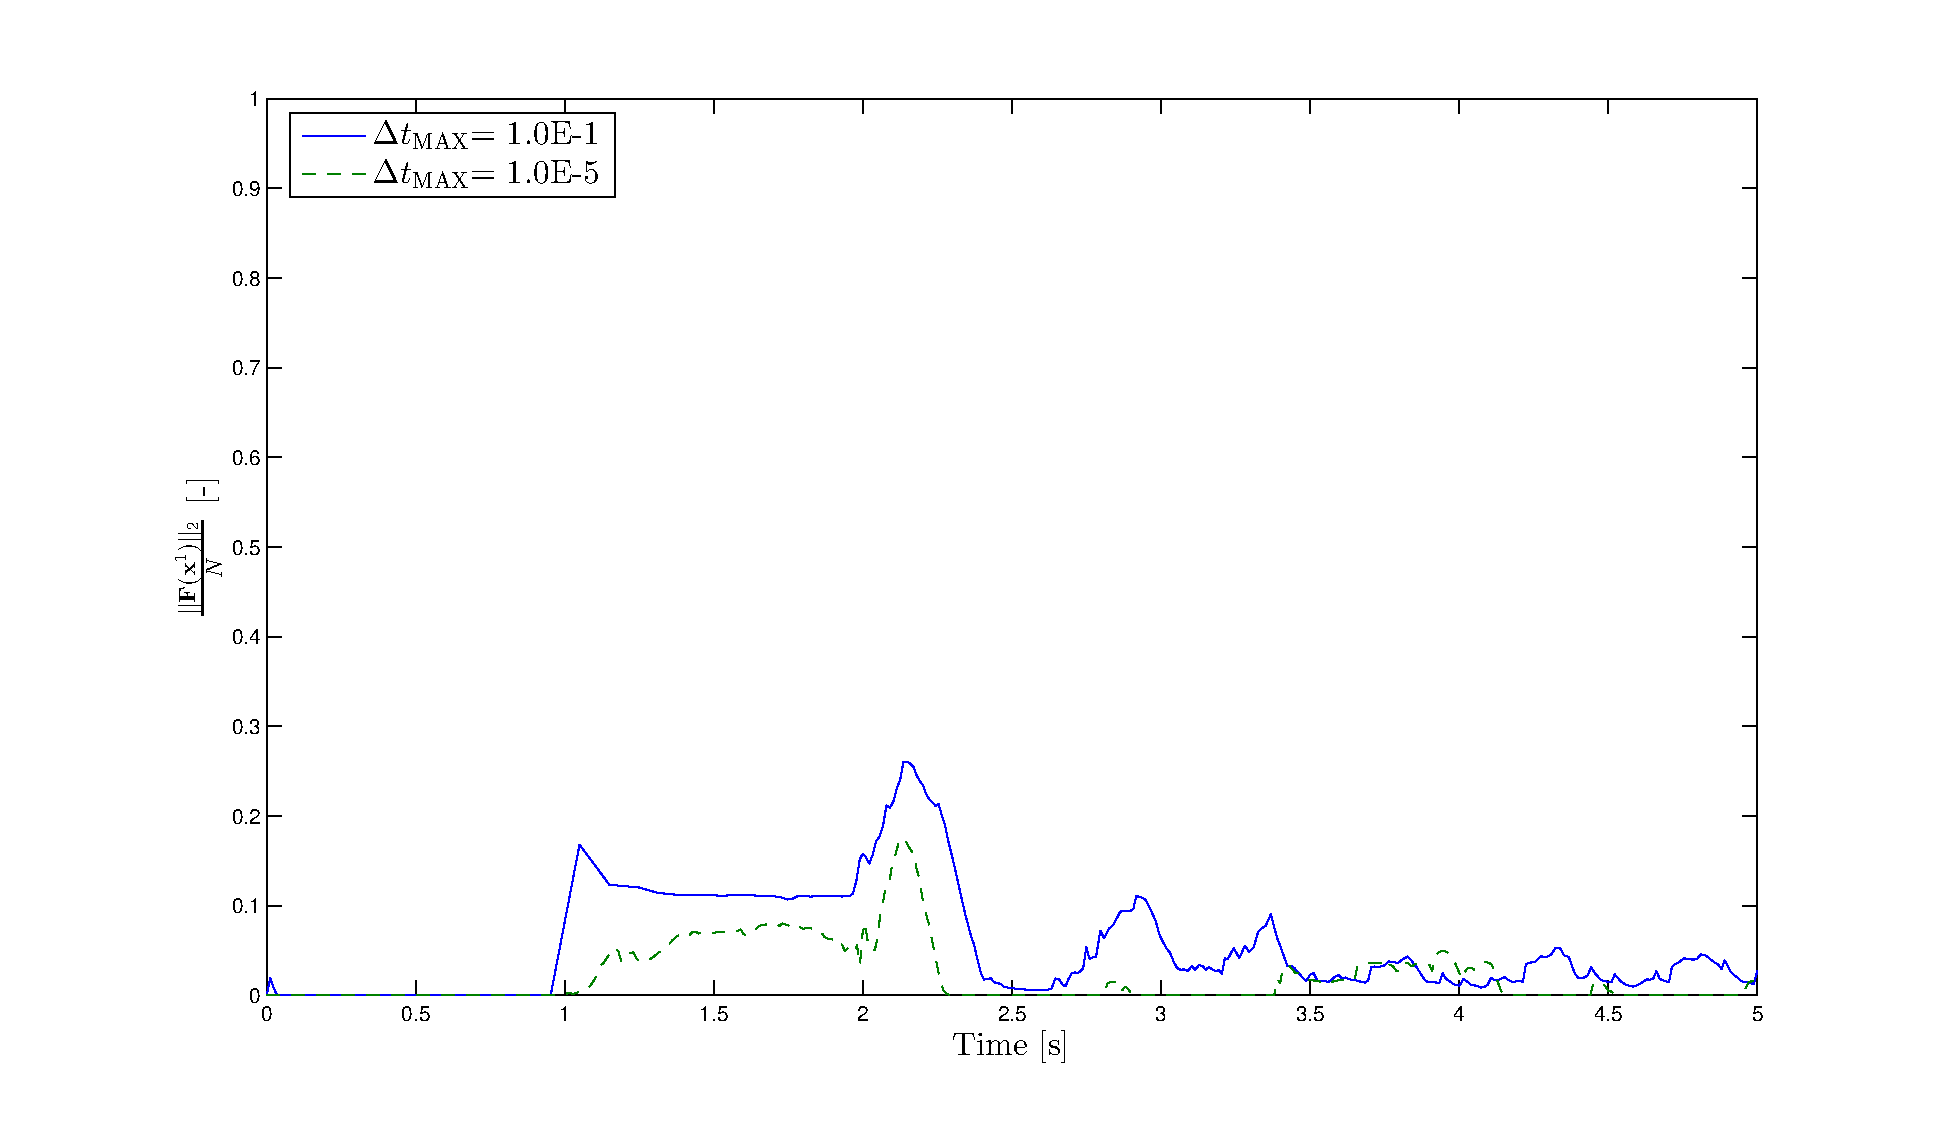
\includegraphics[width=0.94\textwidth]{images/cobra_flashing_res_compare.eps}
\caption{Residual of the flashing solution for the legacy solver.}
\label{fig:legacy_flashing_residual}
\end{figure}

\begin{figure}[h!t]
\centering
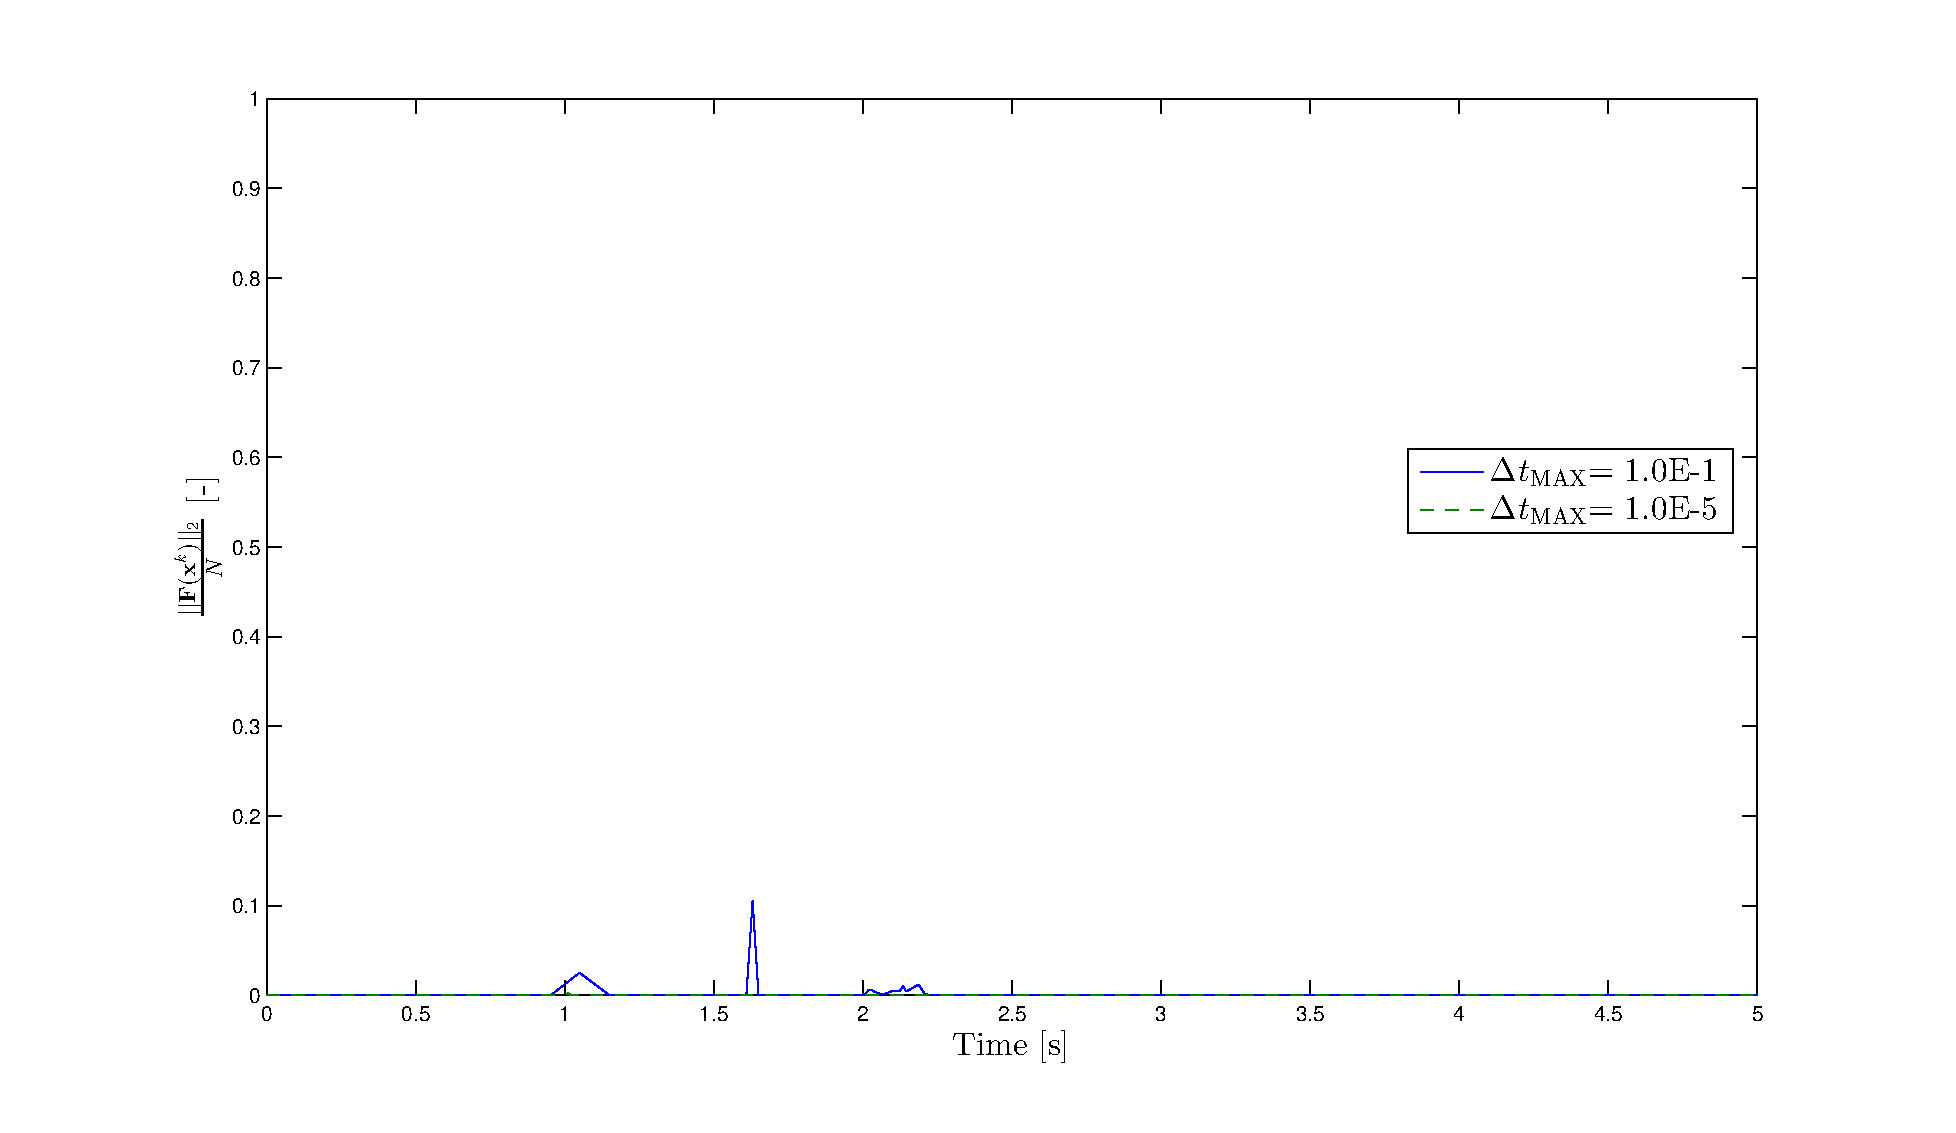
\includegraphics[width=0.94\textwidth]{images/nl_flashing_res_compare.eps}
\caption{Residual of the flashing solution for the nonlinear solver.}
\label{fig:nonlinear_flashing_residual}
\end{figure}

The reduction in the residual exhibited by the solution produced by the legacy solver, \fig{fig:legacy_flashing_residual}, shows that the reduction of the maximum allowable timestep size now serves two purposes.
The first is that as \dtmax{} is reduced the nonlinear physics are being better resolved; however, even for small maximum allowable timestep sizes, the residuals are still large compared to those of the nonlinear solution, \fig{fig:nonlinear_flashing_residual}.
The second purpose in reducing \dtmax{} is to decrease the error due to the discrete approximation of the temporal integral of the governing equations.
While the reduction of the maximum timestep size in the legacy solver serves the purpose of reducing the residual, the nonlinear solver performs this task naturally.
Therefore, in the nonlinear solver the reduction of the maximum timestep size primarily serves to reduce the error from the approximate discrete temporal integral.

During simulations with large \dtmax{} there are three time periods of the transient where the residuals from the nonlinear solver are nontrivial.
These are at the initiation of the inlet flow, during the 1 [s] long ramp to full flow, and after the inlet flow has achieved steady state at 2 [s].
The convergence criteria outlined in \sect{sect:nl_cobra} include two paths through which Newton's method may terminate while having a non-trivial residual.
The first is that the maximum allowable number of Newton iterates, $k_{\text{MAX}}$, may have been exceeded. 
This may indicate that $k_{\text{MAX}}$ may be too small, terminating the iterative process prior to a solution being obtained.
The second is that the norm of the scaled independent parameter update vector may be below its convergence threshold.
A concern is that the update vector produced by the Newton step may be truncated based upon the limiting of the independent parameters at the end of a Newton step.
It may be impossible for the algorithm to reach a nonlinearly converged solution without pushing an independent parameter outside of the acceptable limits imposed by the software.
Since the global minimization problem is not formulated as a constrained minimization problem, there may be inconsistencies in the solution.
This non-convergence of the residual needs additional investigation to determine its cause, its impact upon the algorithmic framework, and its possible remedies.

%\begin{figure}[h!t]
%\centering
%\subfloat[\dtmax{} = 1.0 {[s]}]{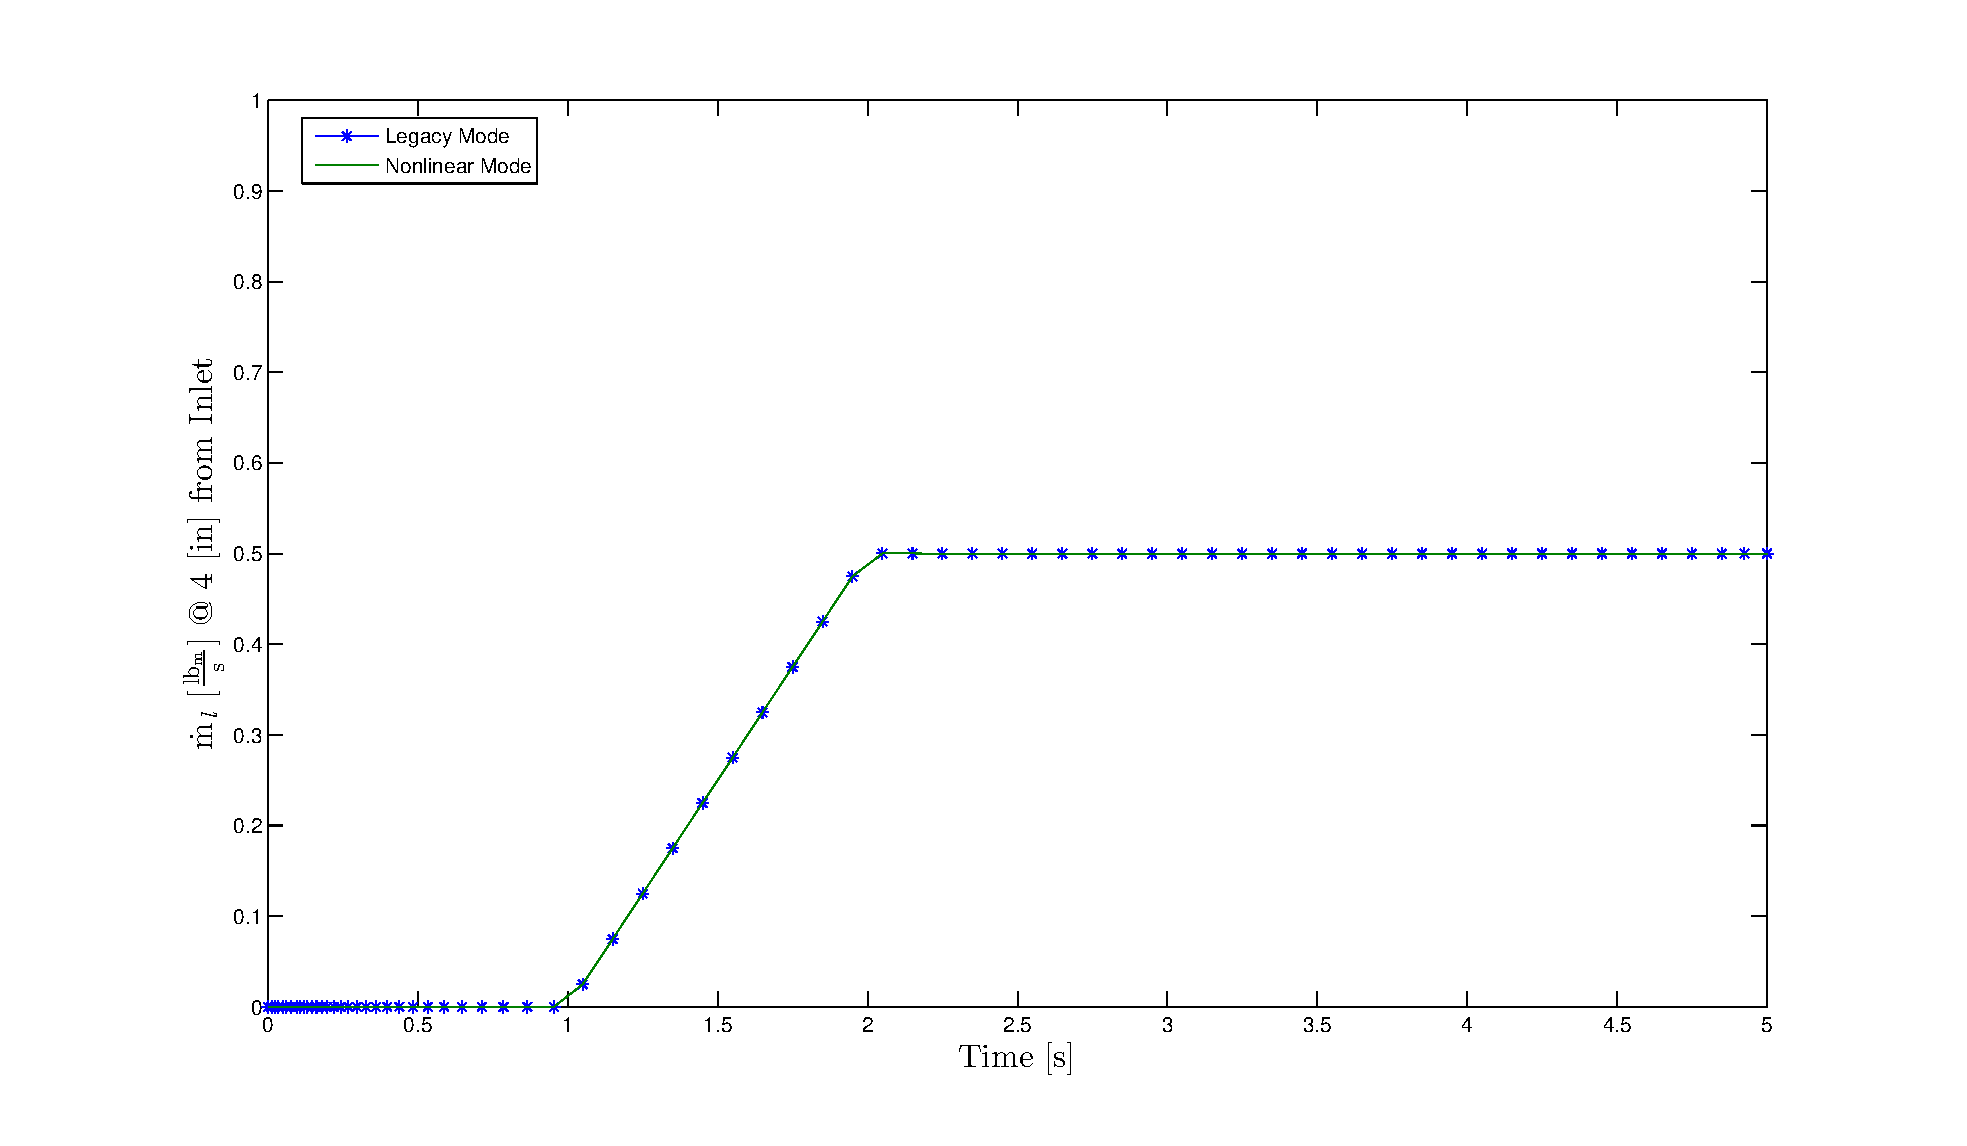
\includegraphics[width=0.49\textwidth]{images/single_1em0.eps}
%\label{fig:single_1em1}}
%\subfloat[\dtmax{} = 1.0E-5 {[s]}]{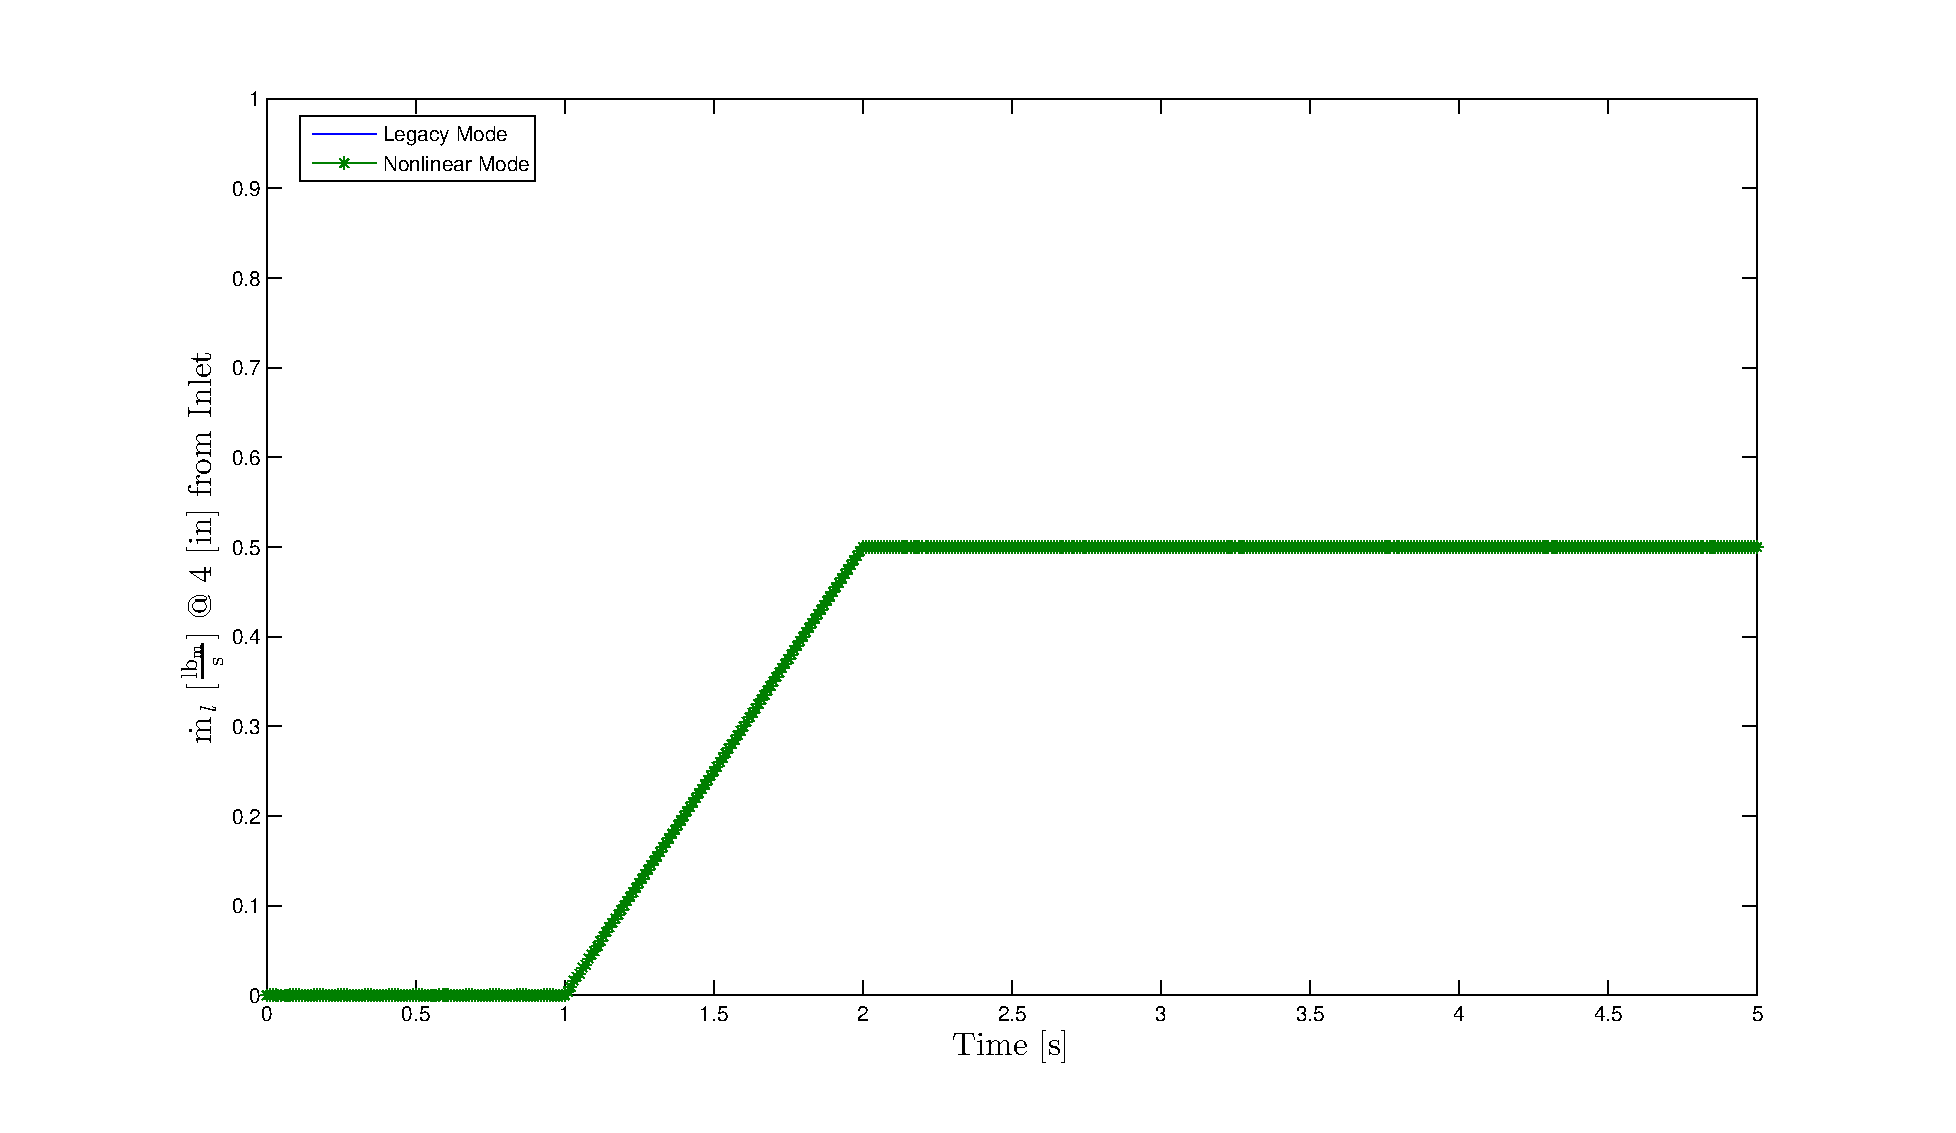
\includegraphics[width=0.49\textwidth]{images/single_1em5.eps}
%\label{fig:single_1em5}}
%\caption[Single-phase solution at \dtmax{} = 1.0 {[s]}and 1.0E-5 {[s]}]{Single-phase solution with \dtmax{} = 1.0 {[s]} and 1.0E-5 {[s]}.}
%\label{fig:single_compare_1}
%\end{figure}

\begin{figure}[h!t]
\centering
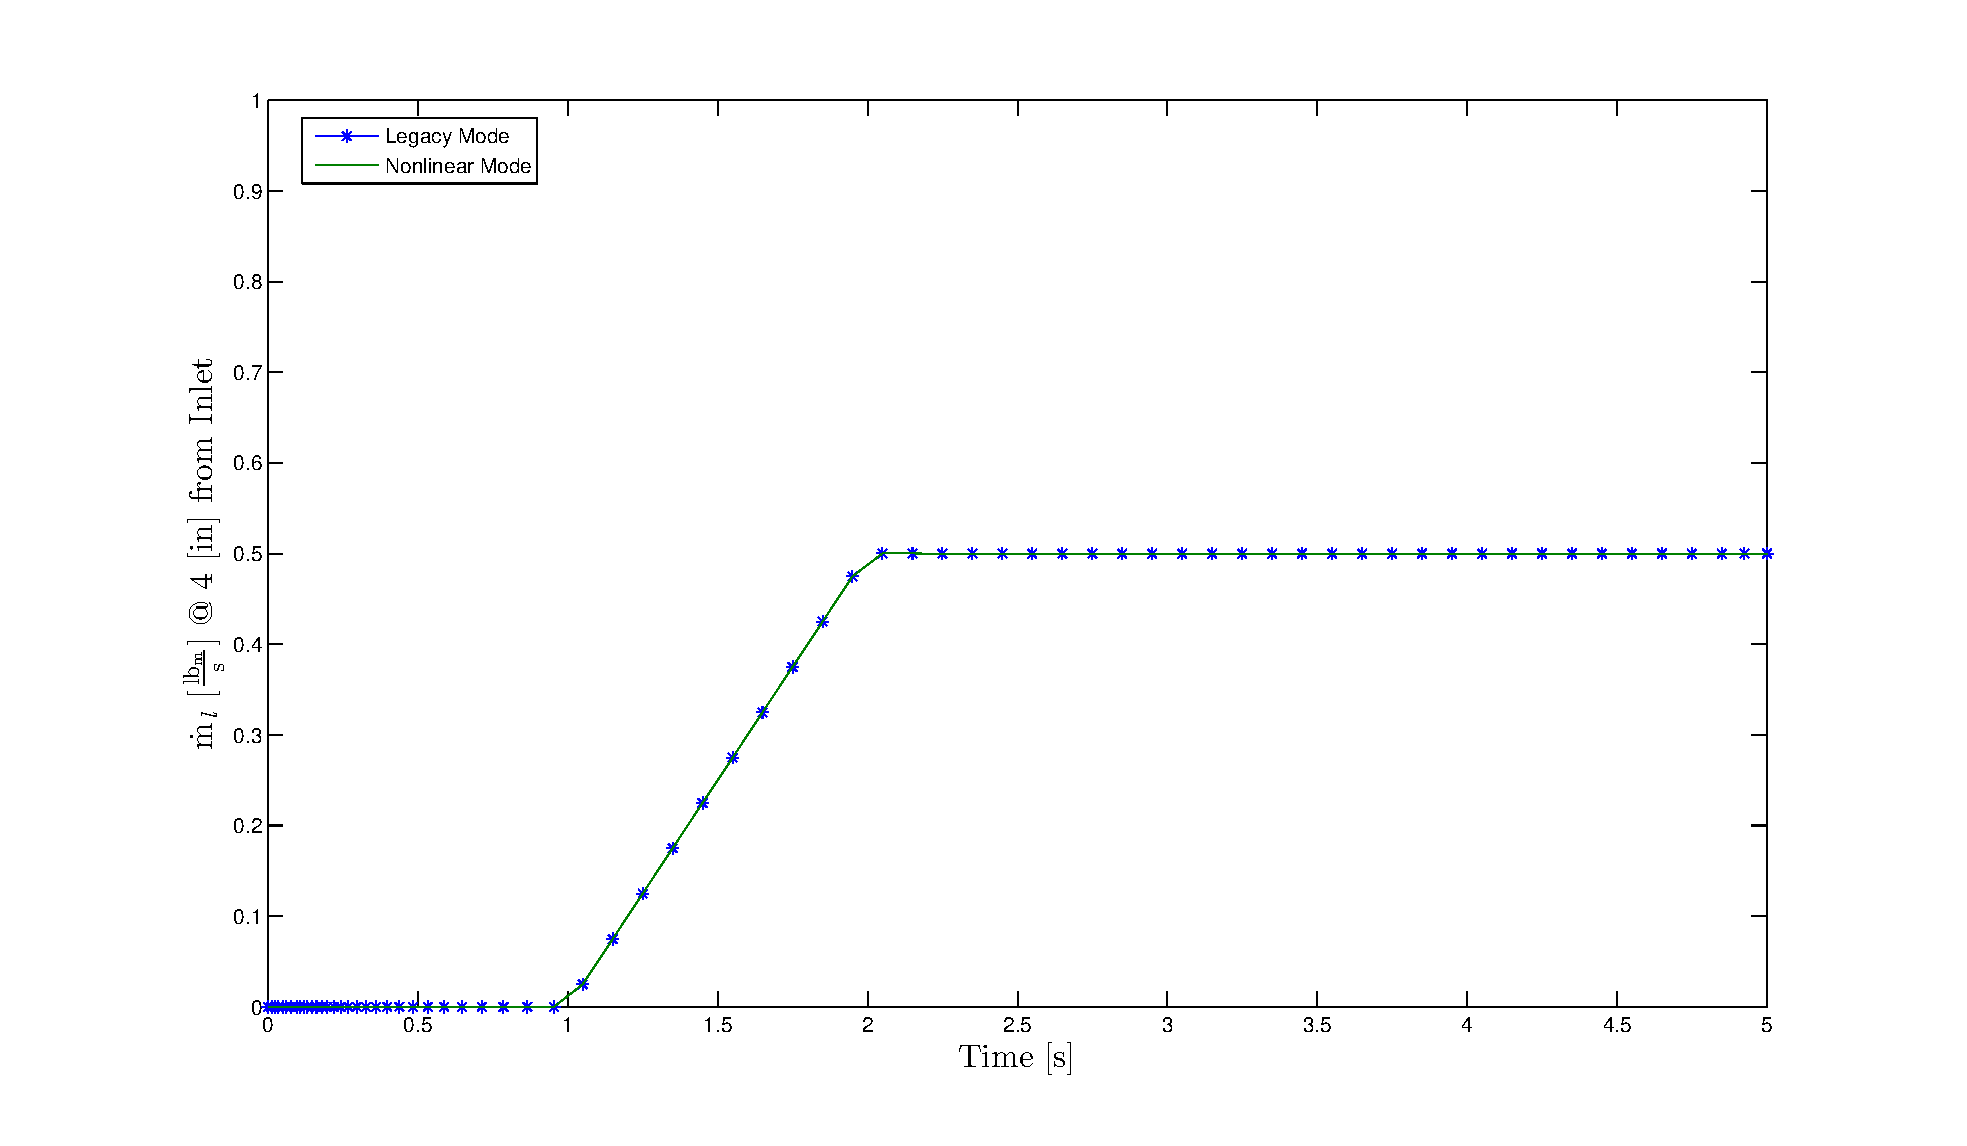
\includegraphics[width=0.94\textwidth]{images/single_1em0.eps}
\caption{Single-phase solution with \dtmax{} = 1.0 {[s]}.}
\label{fig:single_1em1}
\end{figure}

\begin{figure}[h!t]
\centering
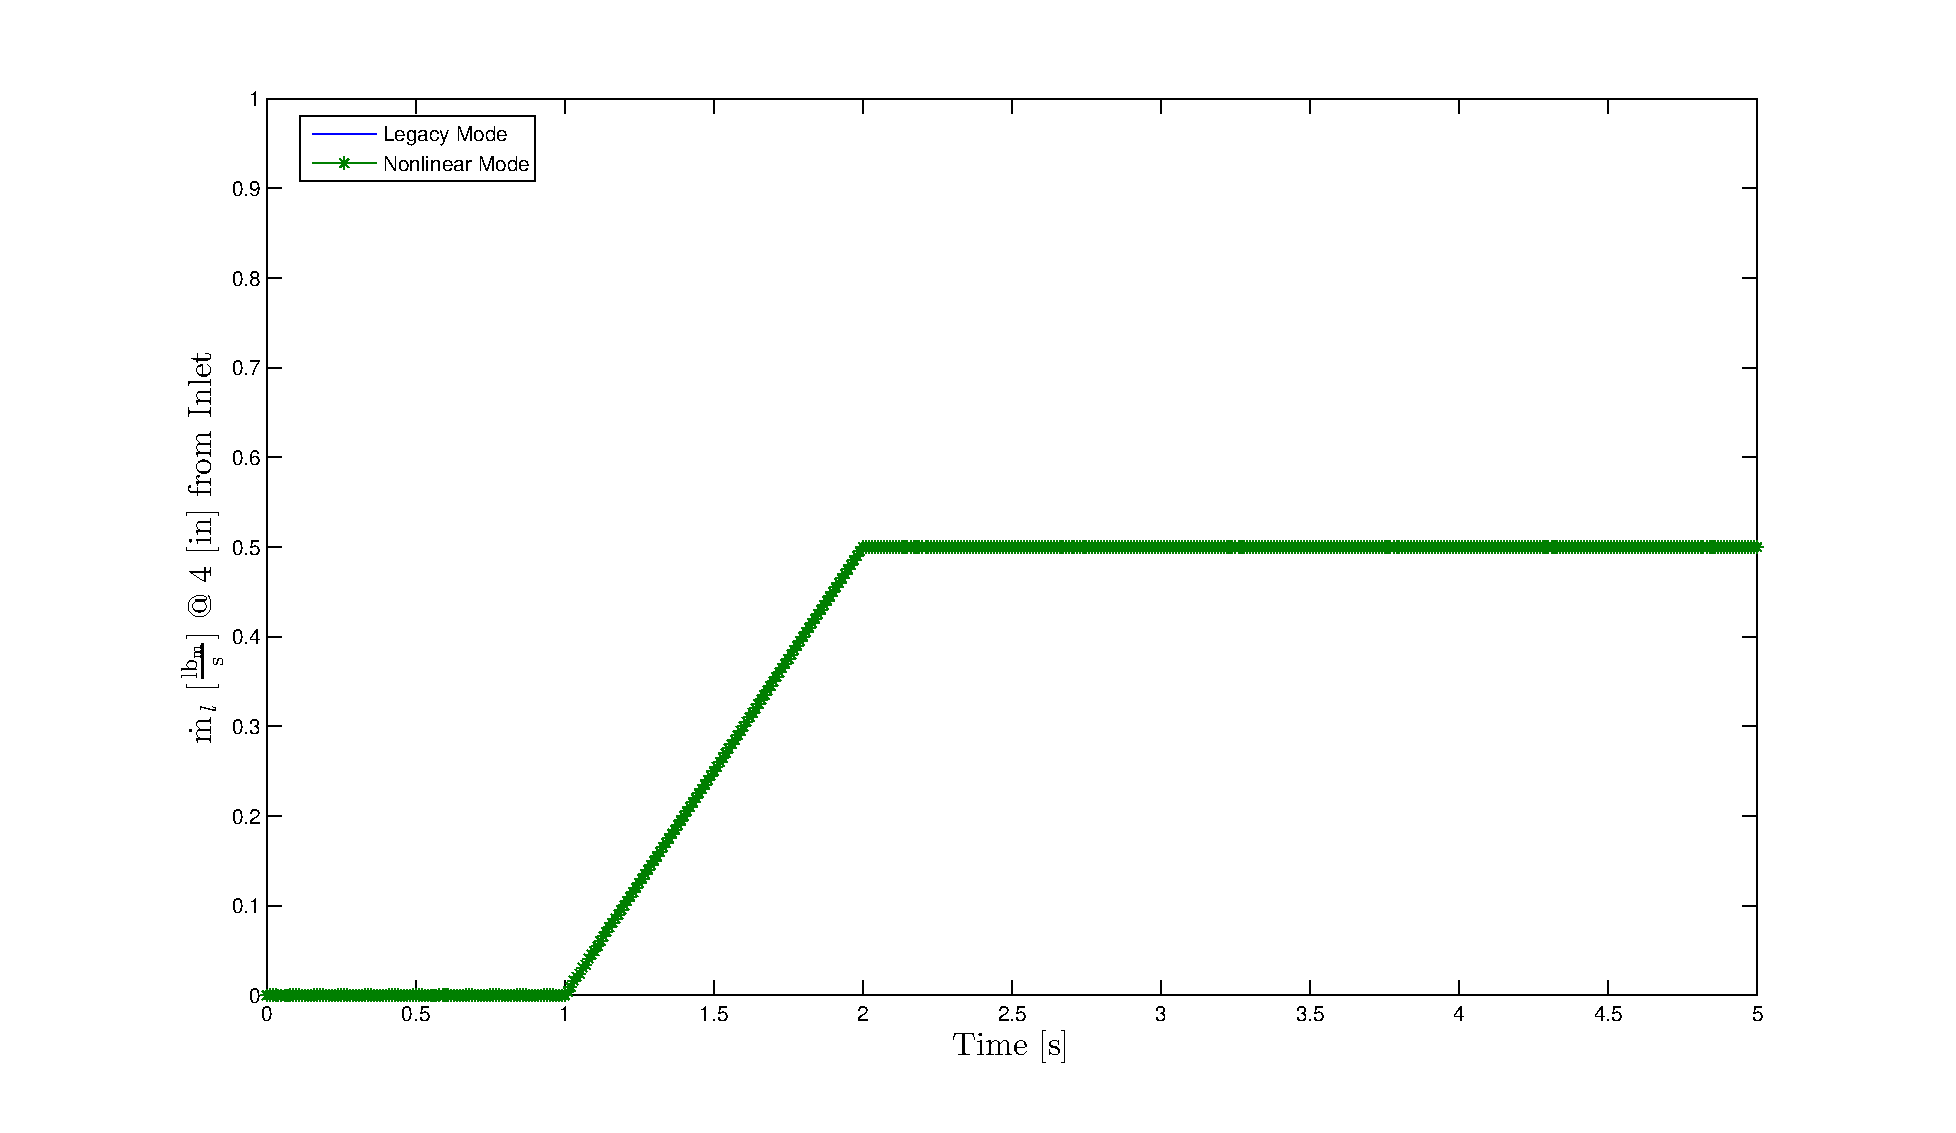
\includegraphics[width=0.94\textwidth]{images/single_1em5.eps}
\caption{Single-phase solution with \dtmax{} = 1.0E-5 {[s]}.}
\label{fig:single_1em5}
\end{figure}

The single-phase case was designed to test if the legacy solver produced a simulation result that was equivalent to that produced by the nonlinear solver.
More specifically, it was designed to show that for problems where the physics of interest have relatively low nonlinearities, the legacy solver provides as accurate a solution as the nonlinear solver.
\fig{fig:single_1em1} and \fig{fig:single_1em5} show the solution produced by both the nonlinear and legacy solvers of \cobra{}.
Unlike the flashing problem, both solvers were able to solve the problem for all of the \dtmax{} specified.
The solutions produced by both solvers are qualitatively equivalent at \dtmax{} = 1.0 [s] and \dtmax{} = 1.0E-5 [s].
This indicates that the legacy solver is adequate in regions where the solution is not highly nonlinear.

%\begin{figure}[h!t]
%\centering
%\subfloat[Legacy mode.]
%{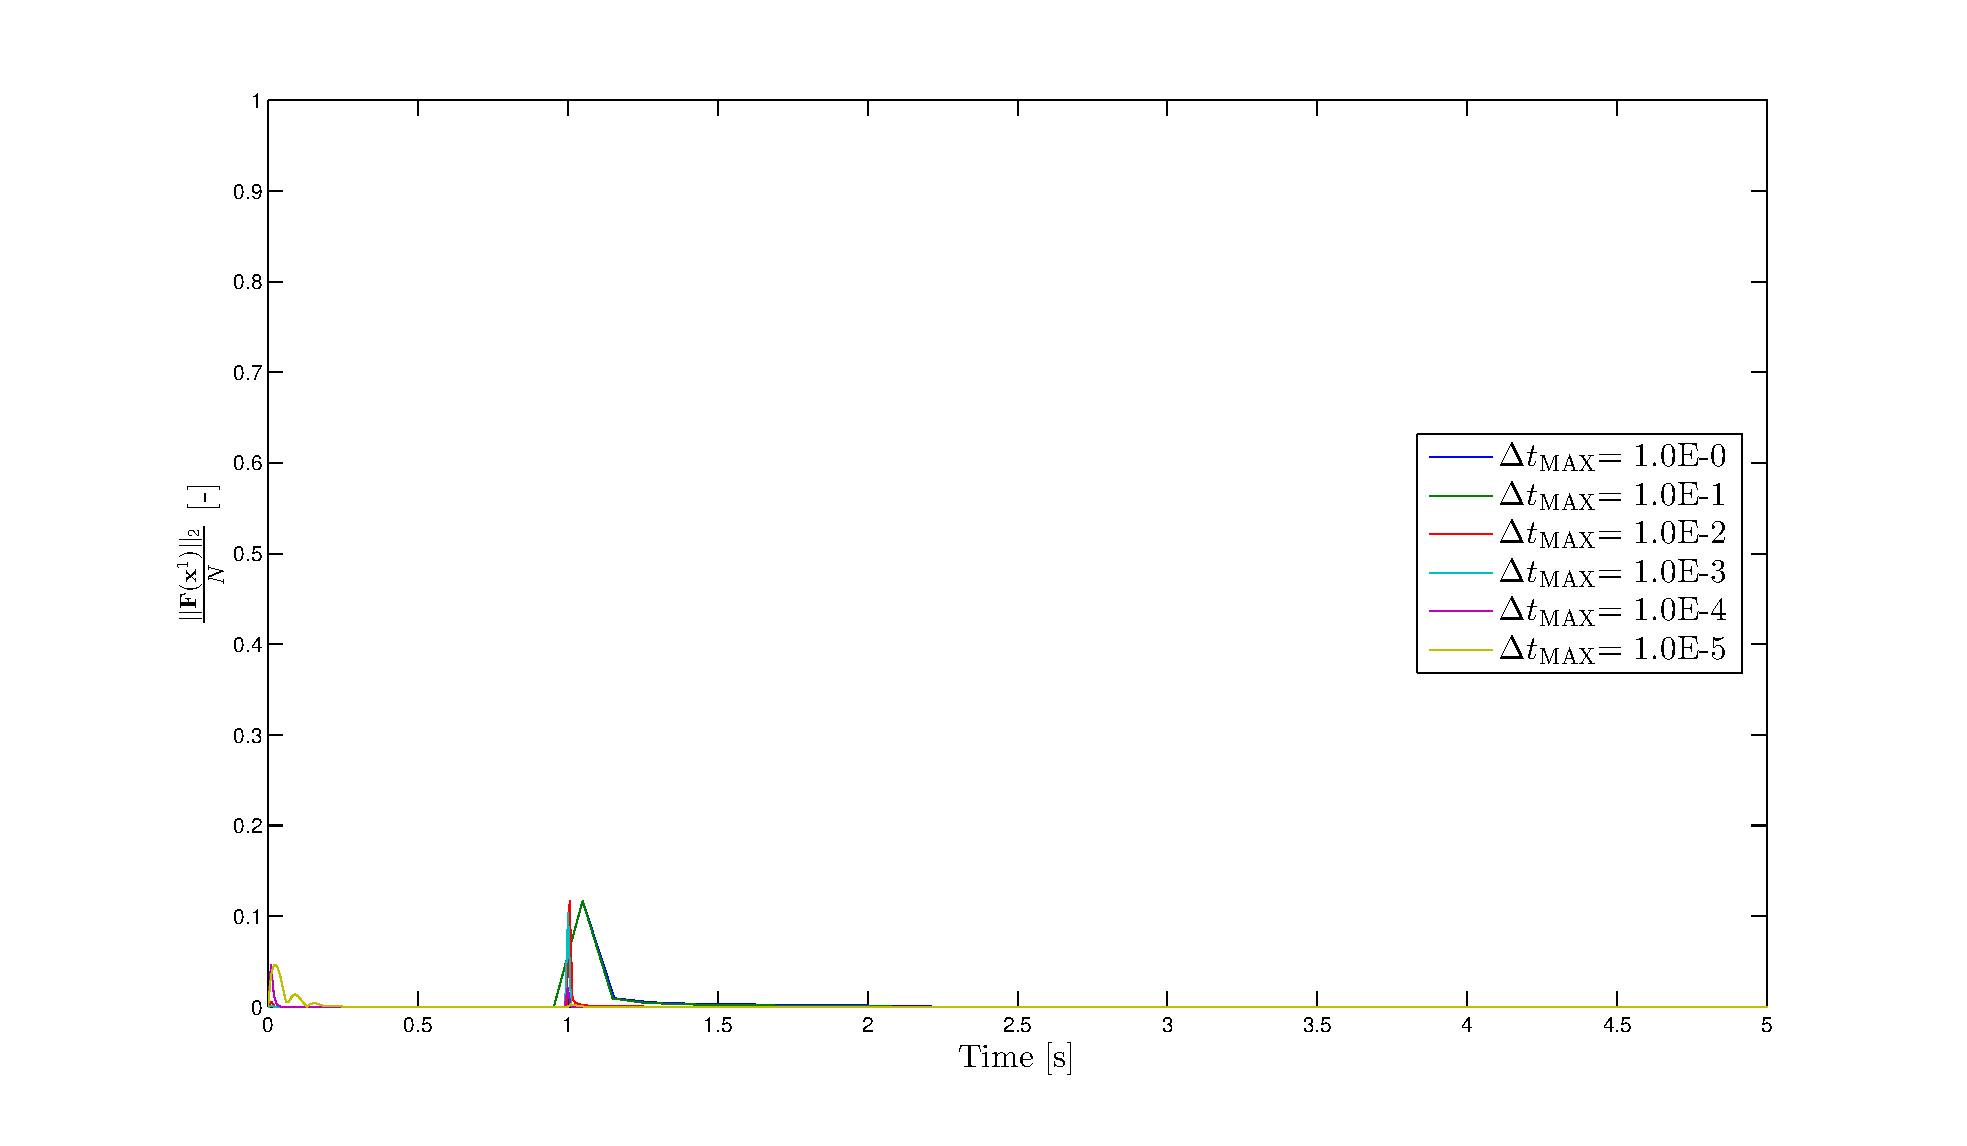
\includegraphics[width=0.49\textwidth]{images/cobra_single_res_v_dt.eps}
%\label{fig:leg_single_res}}
%\subfloat[Nonlinear mode.]{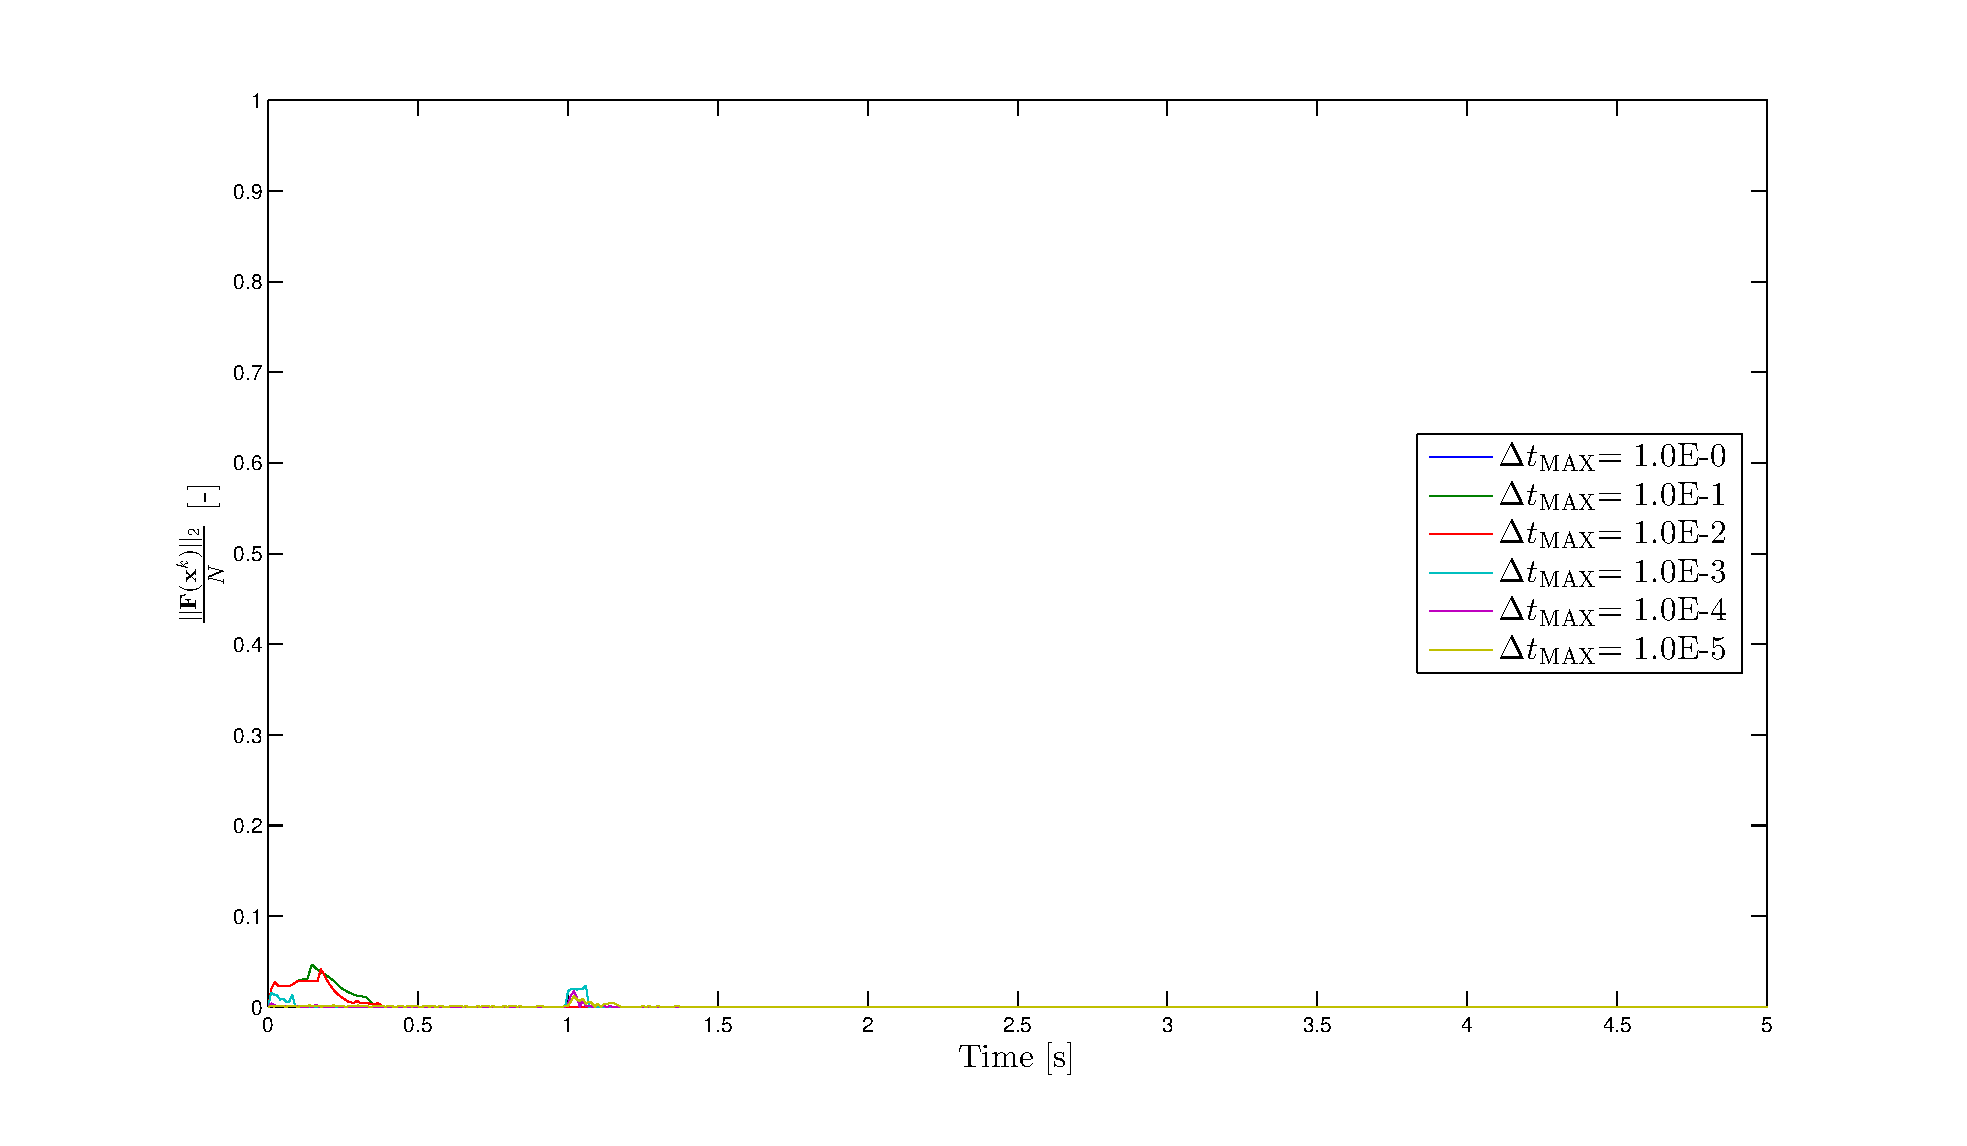
\includegraphics[width=0.49\textwidth]{images/nl_single_res_v_dt.eps}
%\label{fig:nl_single_res}}
%\caption[Single-phase residuals.]{Single-phase residuals.}
%\label{fig:single_compare_2}
%\end{figure}

\begin{figure}[h!t]
\centering
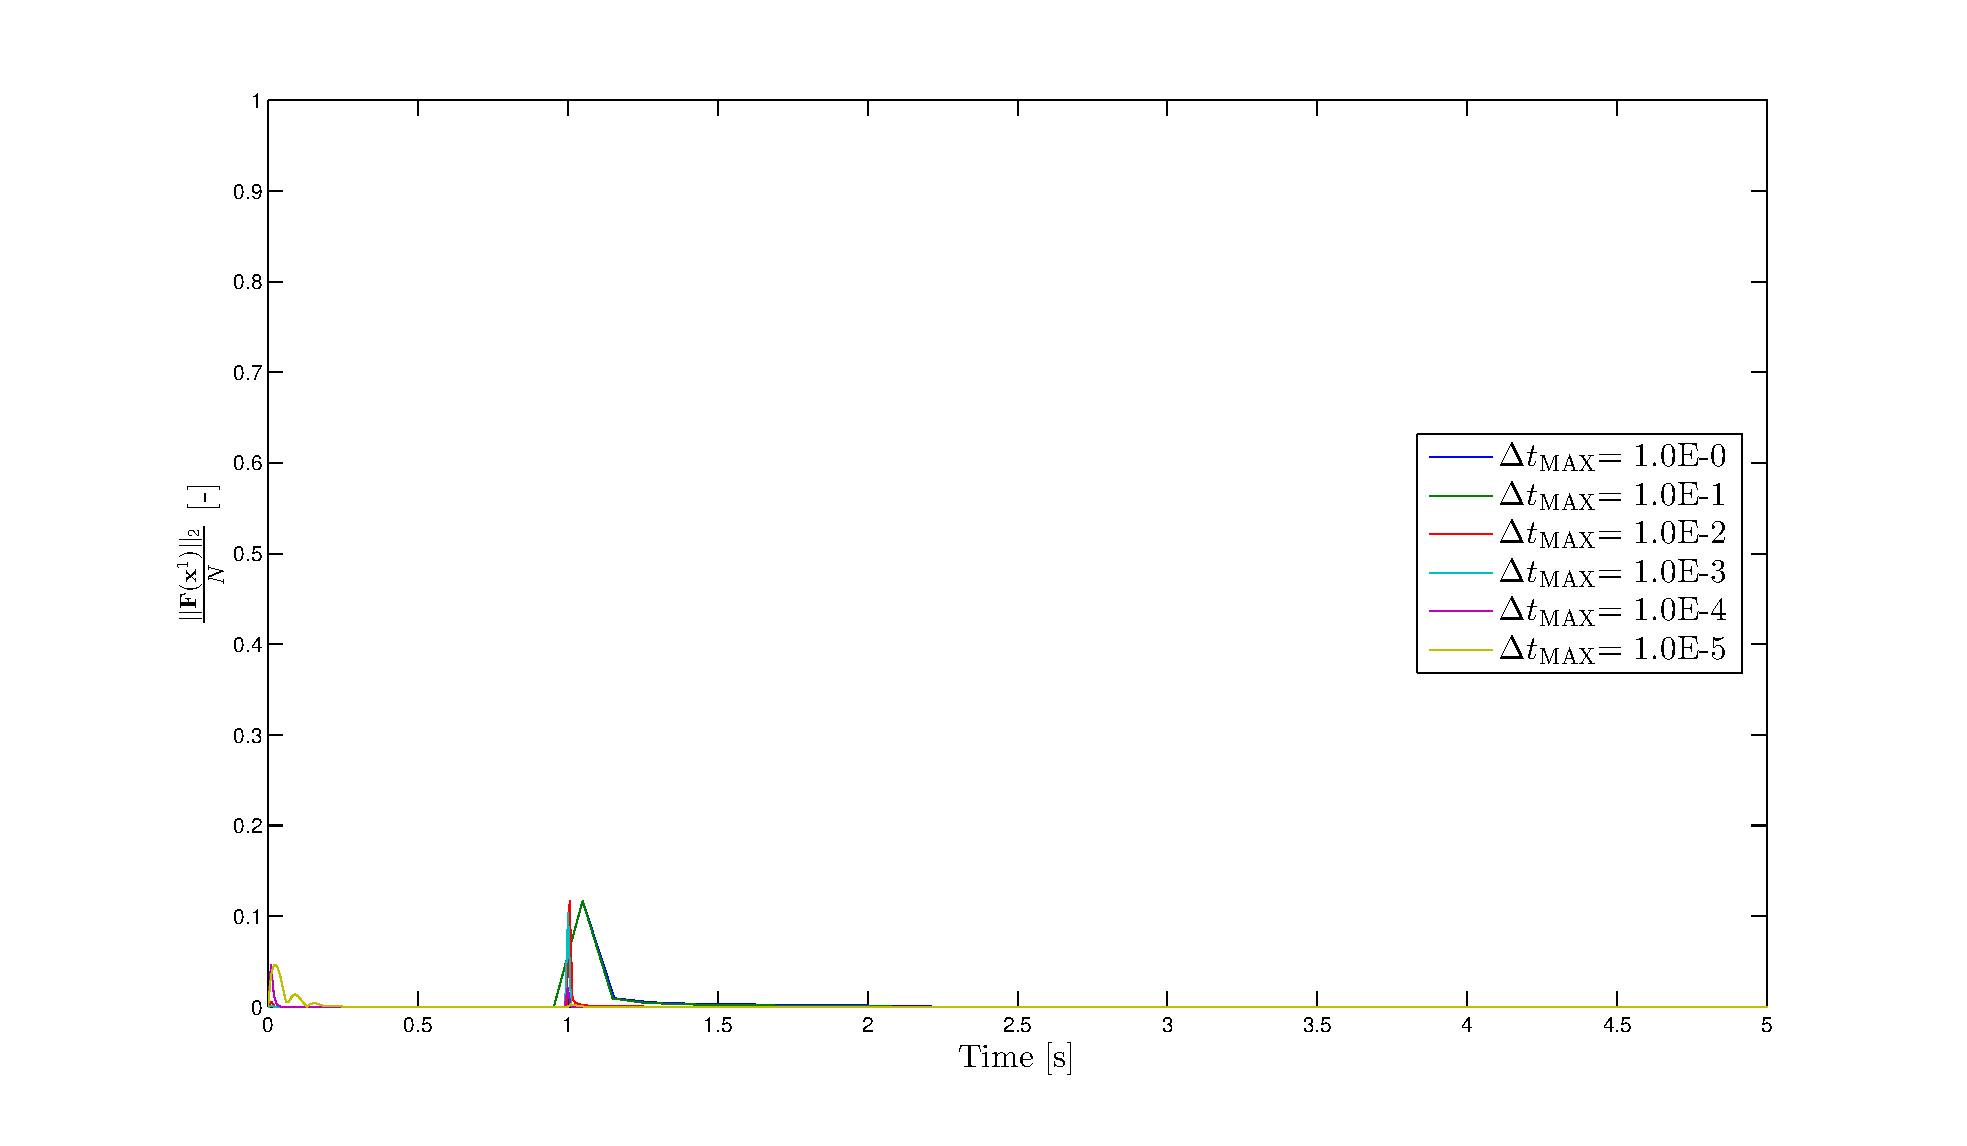
\includegraphics[width=0.94\textwidth]{images/cobra_single_res_v_dt.eps}
\caption{Legacy solver single-phase residuals.}
\label{fig:leg_single_res}
\end{figure}

\begin{figure}[h!t]
\centering
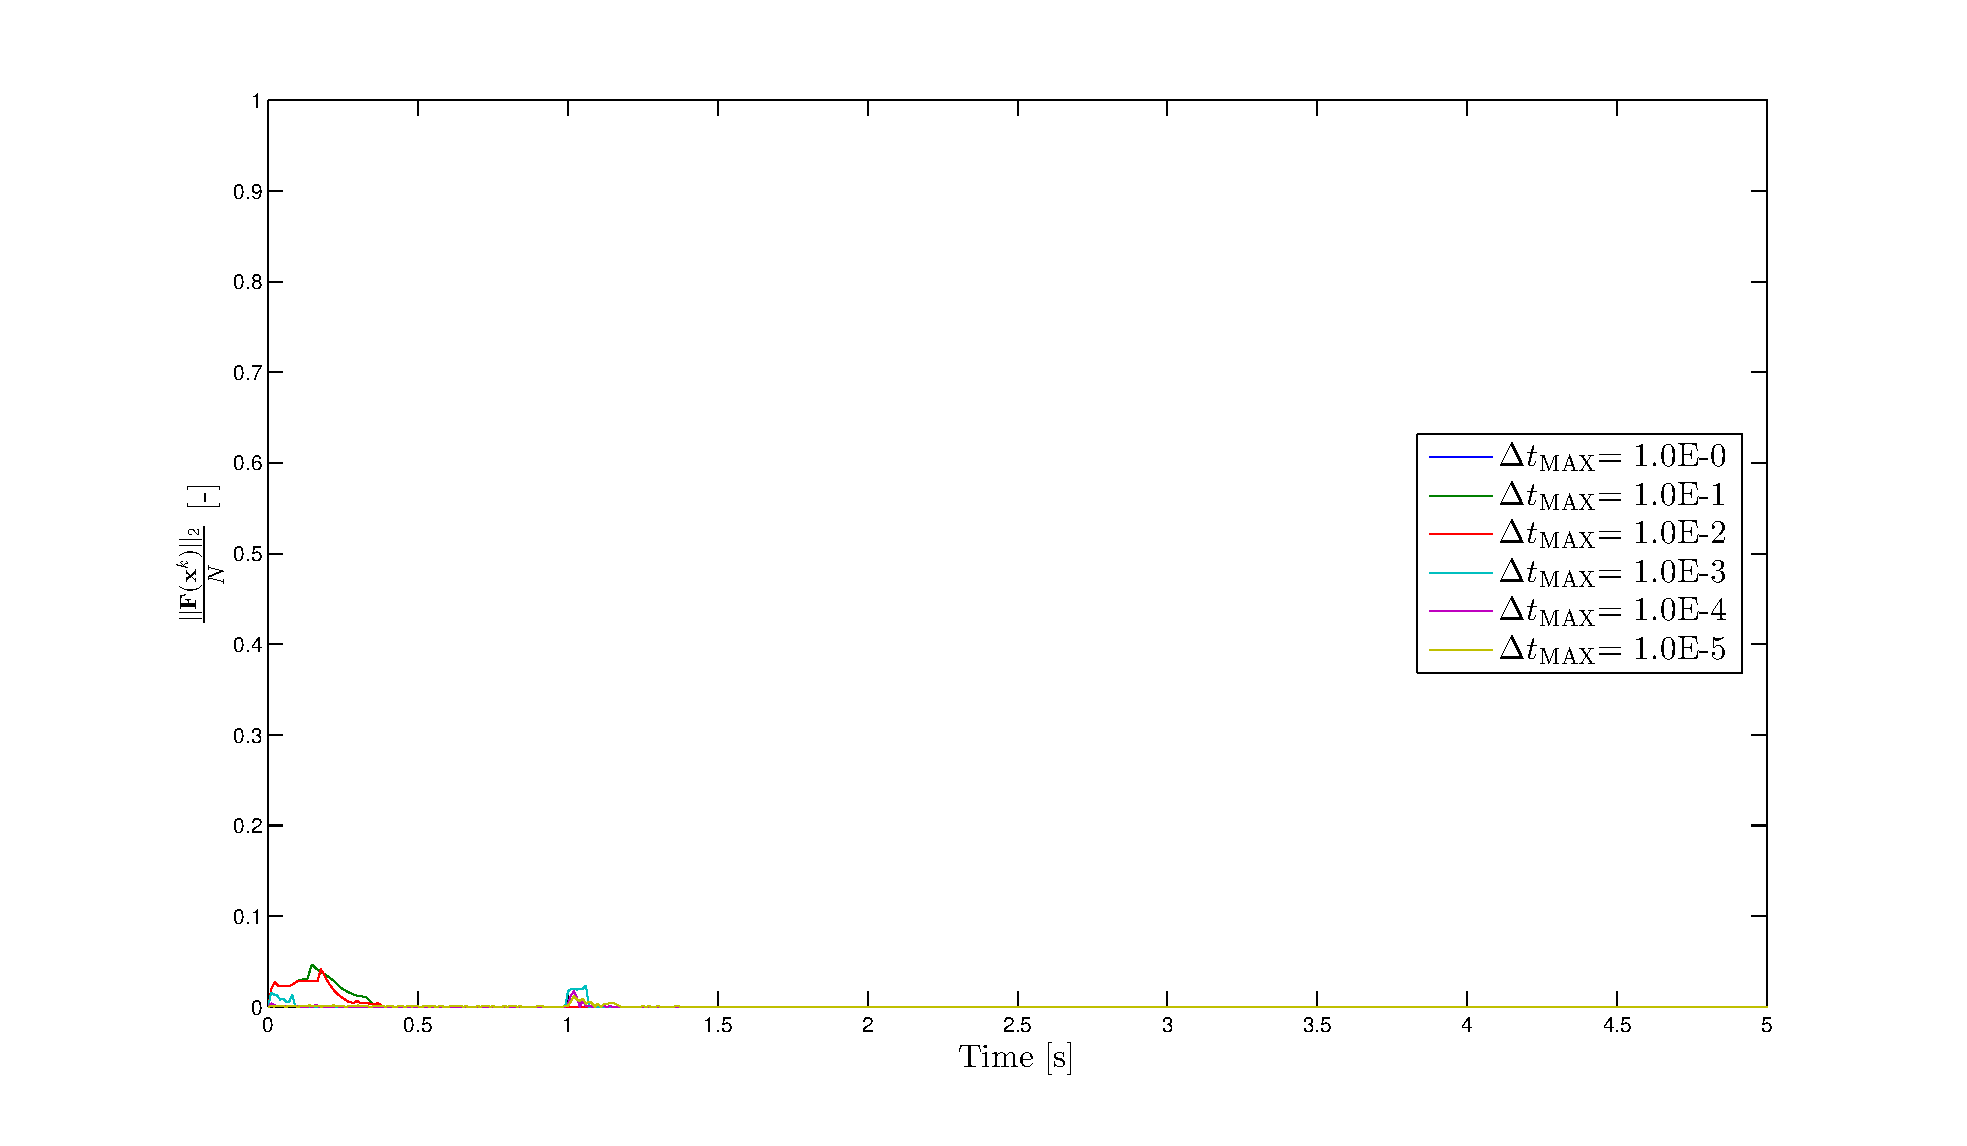
\includegraphics[width=0.94\textwidth]{images/nl_single_res_v_dt.eps}
\caption{Nonlinear solver single-phase residuals.}
\label{fig:nl_single_res}
\end{figure}

Examining the residual for the two different solvers will provide insight into how well each of them are at solving the nonlinear problem.
The residual of the legacy solver solution for the single-phase problem, \fig{fig:leg_single_res}, shows that the nonlinear residuals are nontrivial during two periods of the transient.
The first region of nontrivial residuals is present only for larger values of \dtmax{} and occurs when the the inlet flow initiates at 1 [s].
The second region occurs at smaller values of \dtmax{} and occurs near the beginning of the transient.
For the nonlinear solver solution residuals, \fig{fig:nl_single_res}, the same two regions, the start of simulation and the inlet flow initialization, exhibit similar nontrivial residuals.
However, the behavior of the residual for the nonlinear solver as a function of \dtmax{} exhibits an anomaly that is absent in the legacy solver.
To put the anomaly in context it should first be noted that the nonlinear residual at the initiation of the ramp is approximately zero for \dtmax{} = 1 [s] and \dtmax{} = 1.0E-5 [s].
It is only during intermediate values of \dtmax{} that the residuals becomes nontrivial during the ramp initiation.

%\begin{figure}[h!t]
%\centering
%\subfloat[Transient Solution]{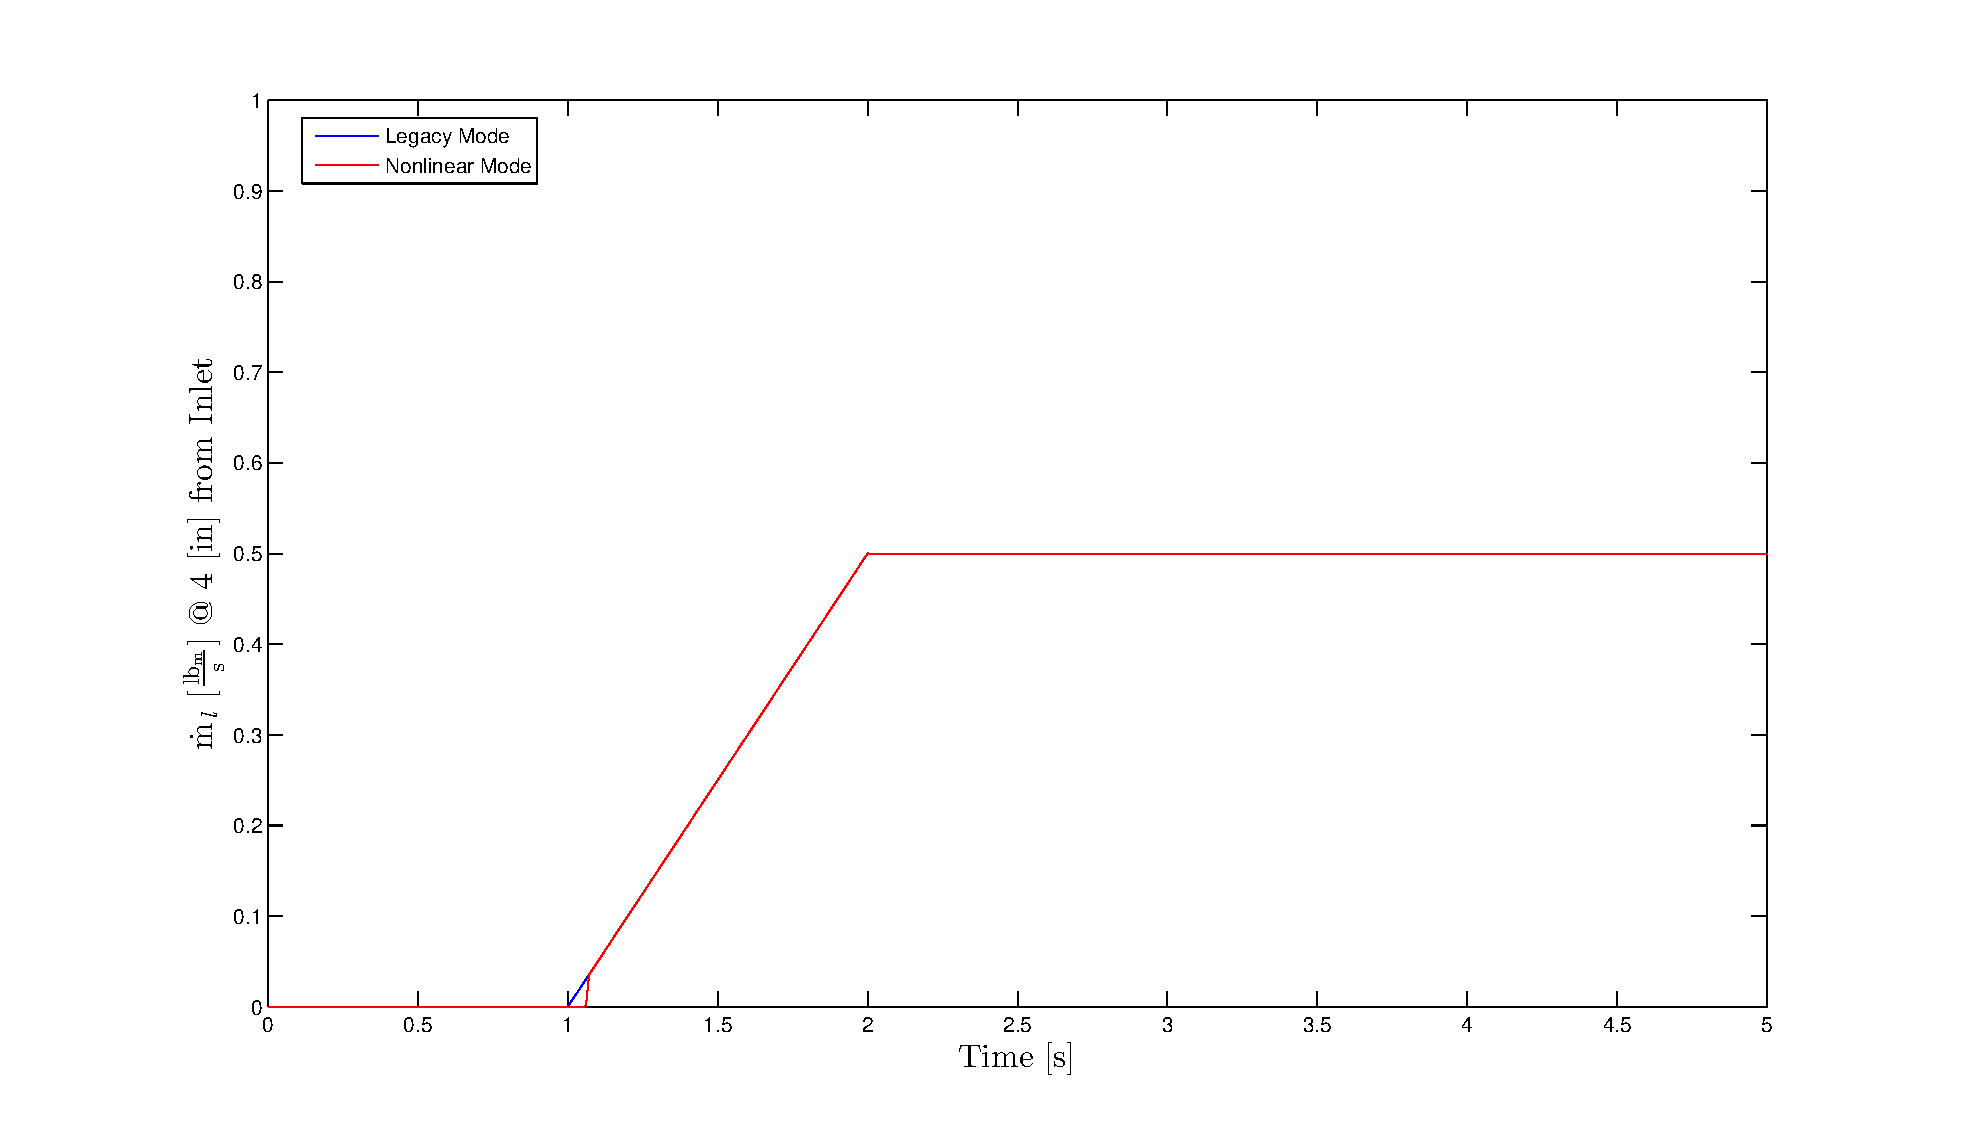
\includegraphics[width=0.49\textwidth]{images/single_1em3.eps}
%\label{fig:single_1em3}}
%\subfloat[Zoomed Solution]{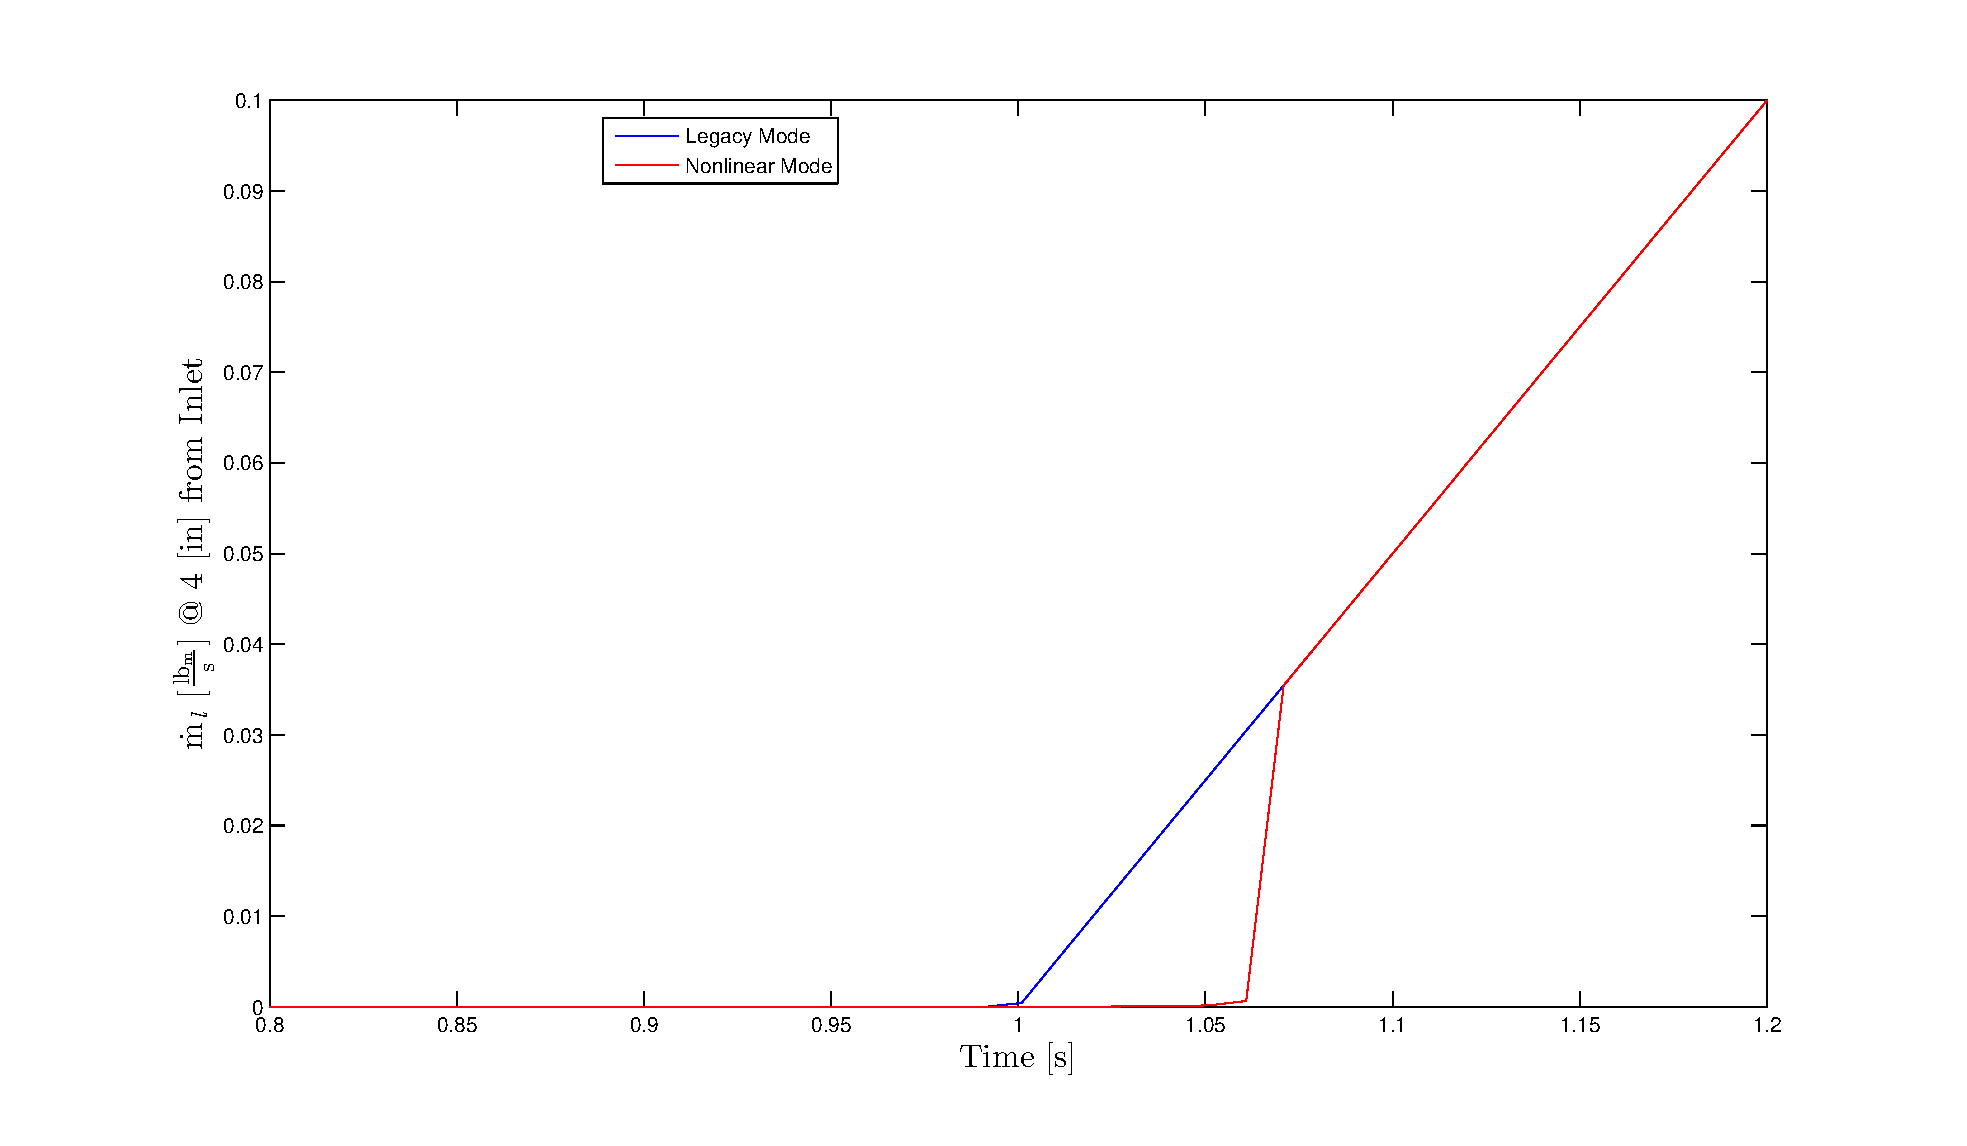
\includegraphics[width=0.49\textwidth]{images/single_1em3_zoom.eps}
%\label{fig:single_1em3_zoom}}
%\caption[Single-phase solution at \dtmax{} = 1.0E-3 {[s]}]{Single-phase solution with \dtmax{} = 1.0E-3 {[s]}.}
%\label{fig:single_compare_3}
%\end{figure}

\begin{figure}[h!t]
\centering
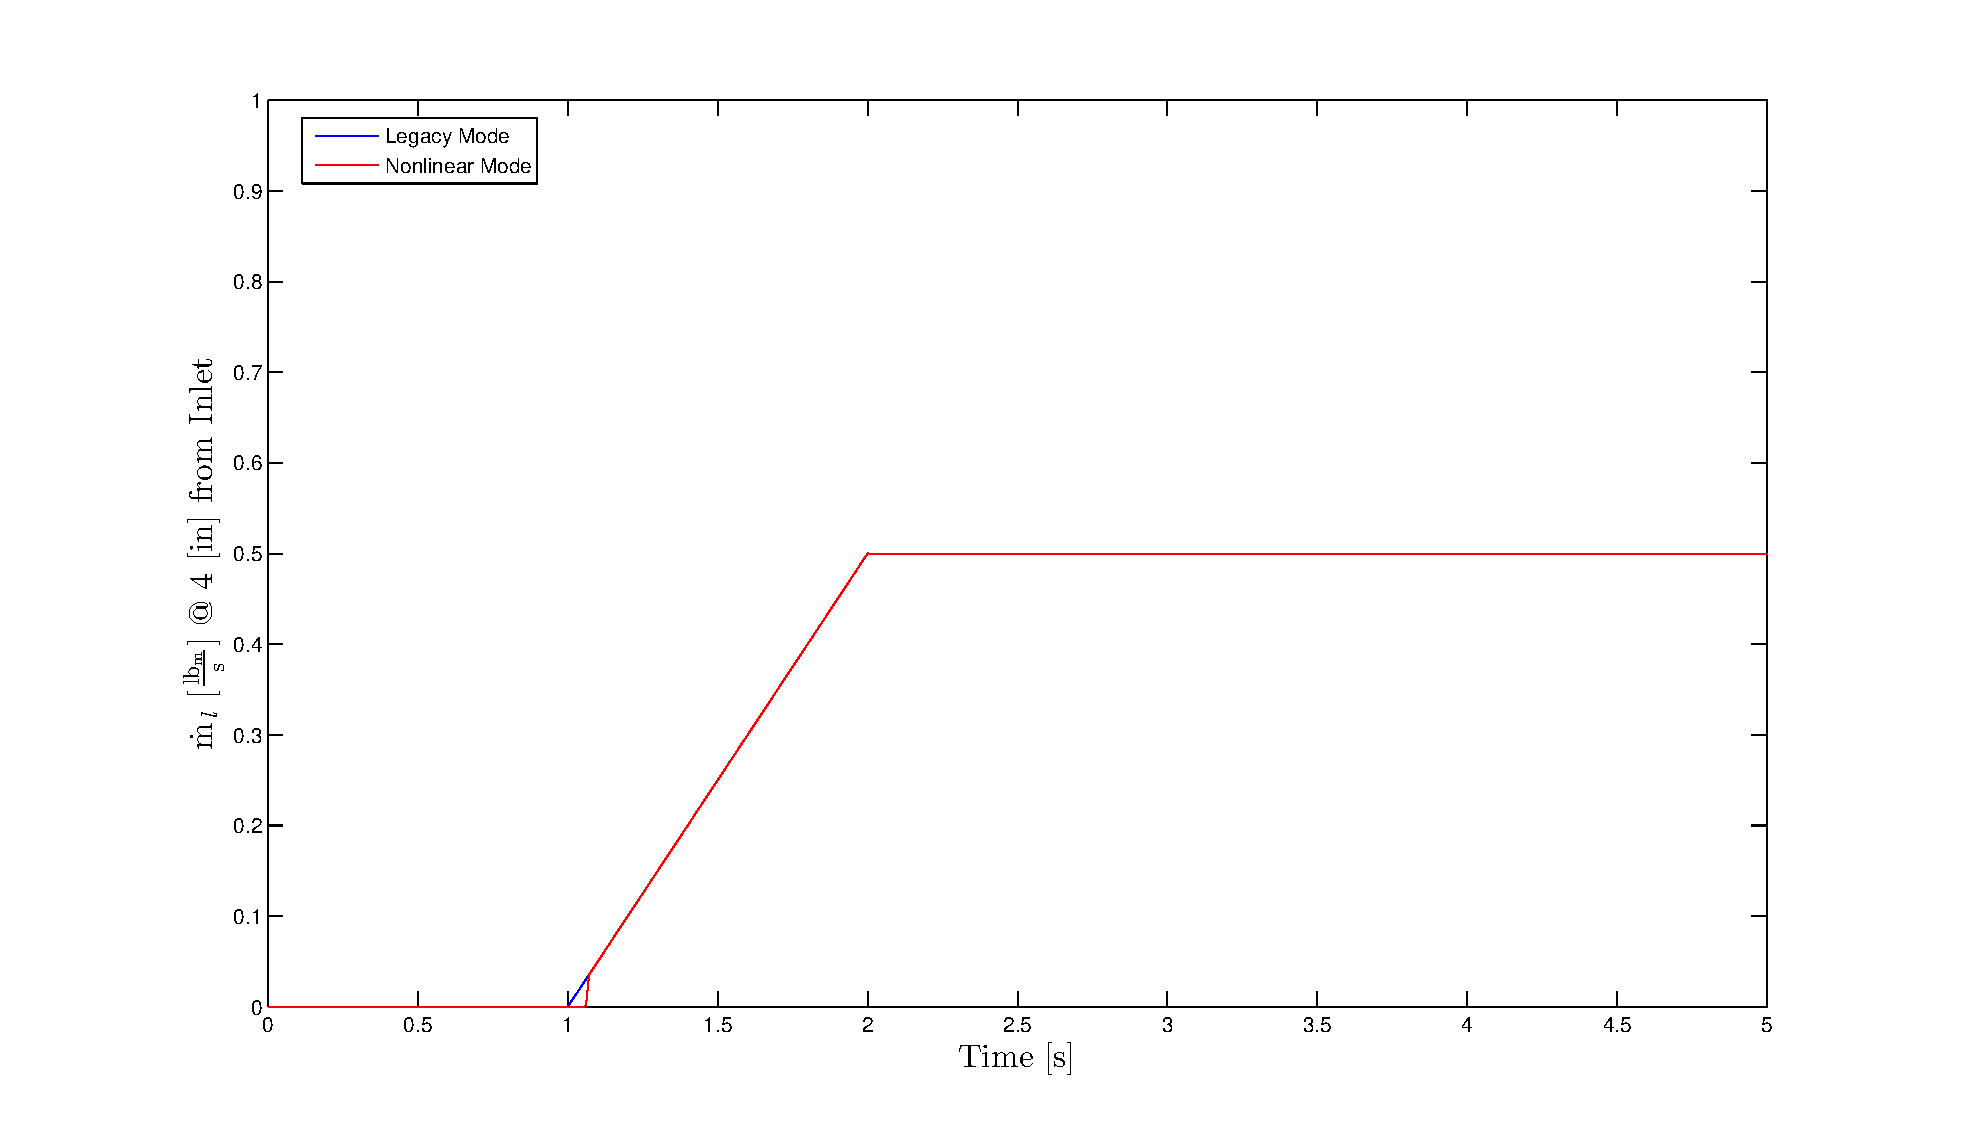
\includegraphics[width=0.94\textwidth]{images/single_1em3.eps}
\caption{Full transient single-phase solution with \dtmax{} = 1.0E-3 {[s]}.}
\label{fig:single_1em3}
\end{figure}

\begin{figure}[h!t]
\centering
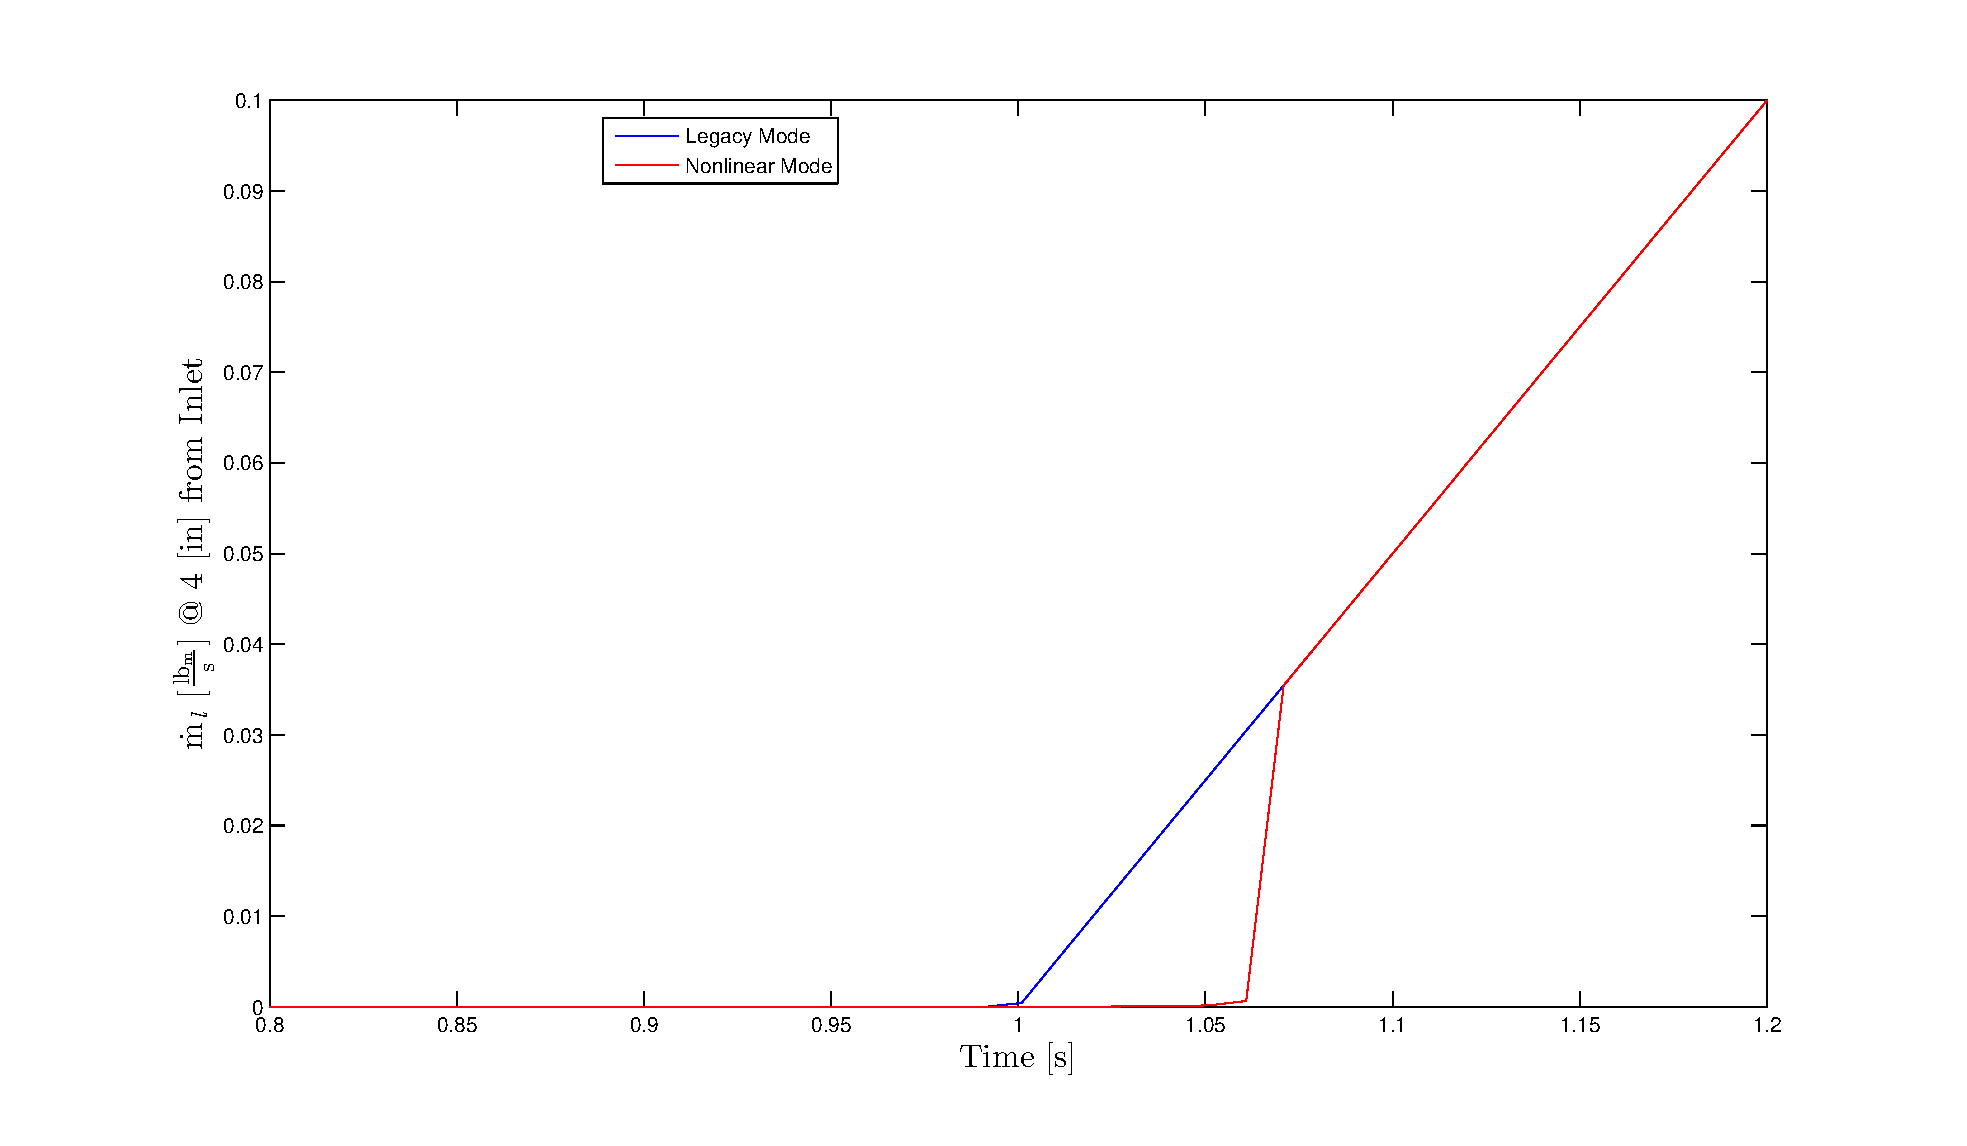
\includegraphics[width=0.94\textwidth]{images/single_1em3_zoom.eps}
\caption{Zoomed single-phase solution with \dtmax{} = 1.0E-3 {[s]}.}
\label{fig:single_1em3_zoom}
\end{figure}

While the solutions at \dtmax{} = 1.0 [s] and \dtmax{} = 1.0E-5 [s] are identical for the two solver modes, the solutions at intermediate timestep sizes were not identical.
In particular, the nonlinear solver produces a solution at \dtmax{} = 1.0E-3 [s] that is inconsistent with both the solution produced by the legacy solver and, more importantly, with the specified inlet boundary conditions.
The two solvers produce solutions that agree for most of the domain, \fig{fig:single_1em3}, except at the initiation of the inlet flow at 1 [s], \fig{fig:single_1em3_zoom}.

%\begin{figure}[h!t]
%\centering
%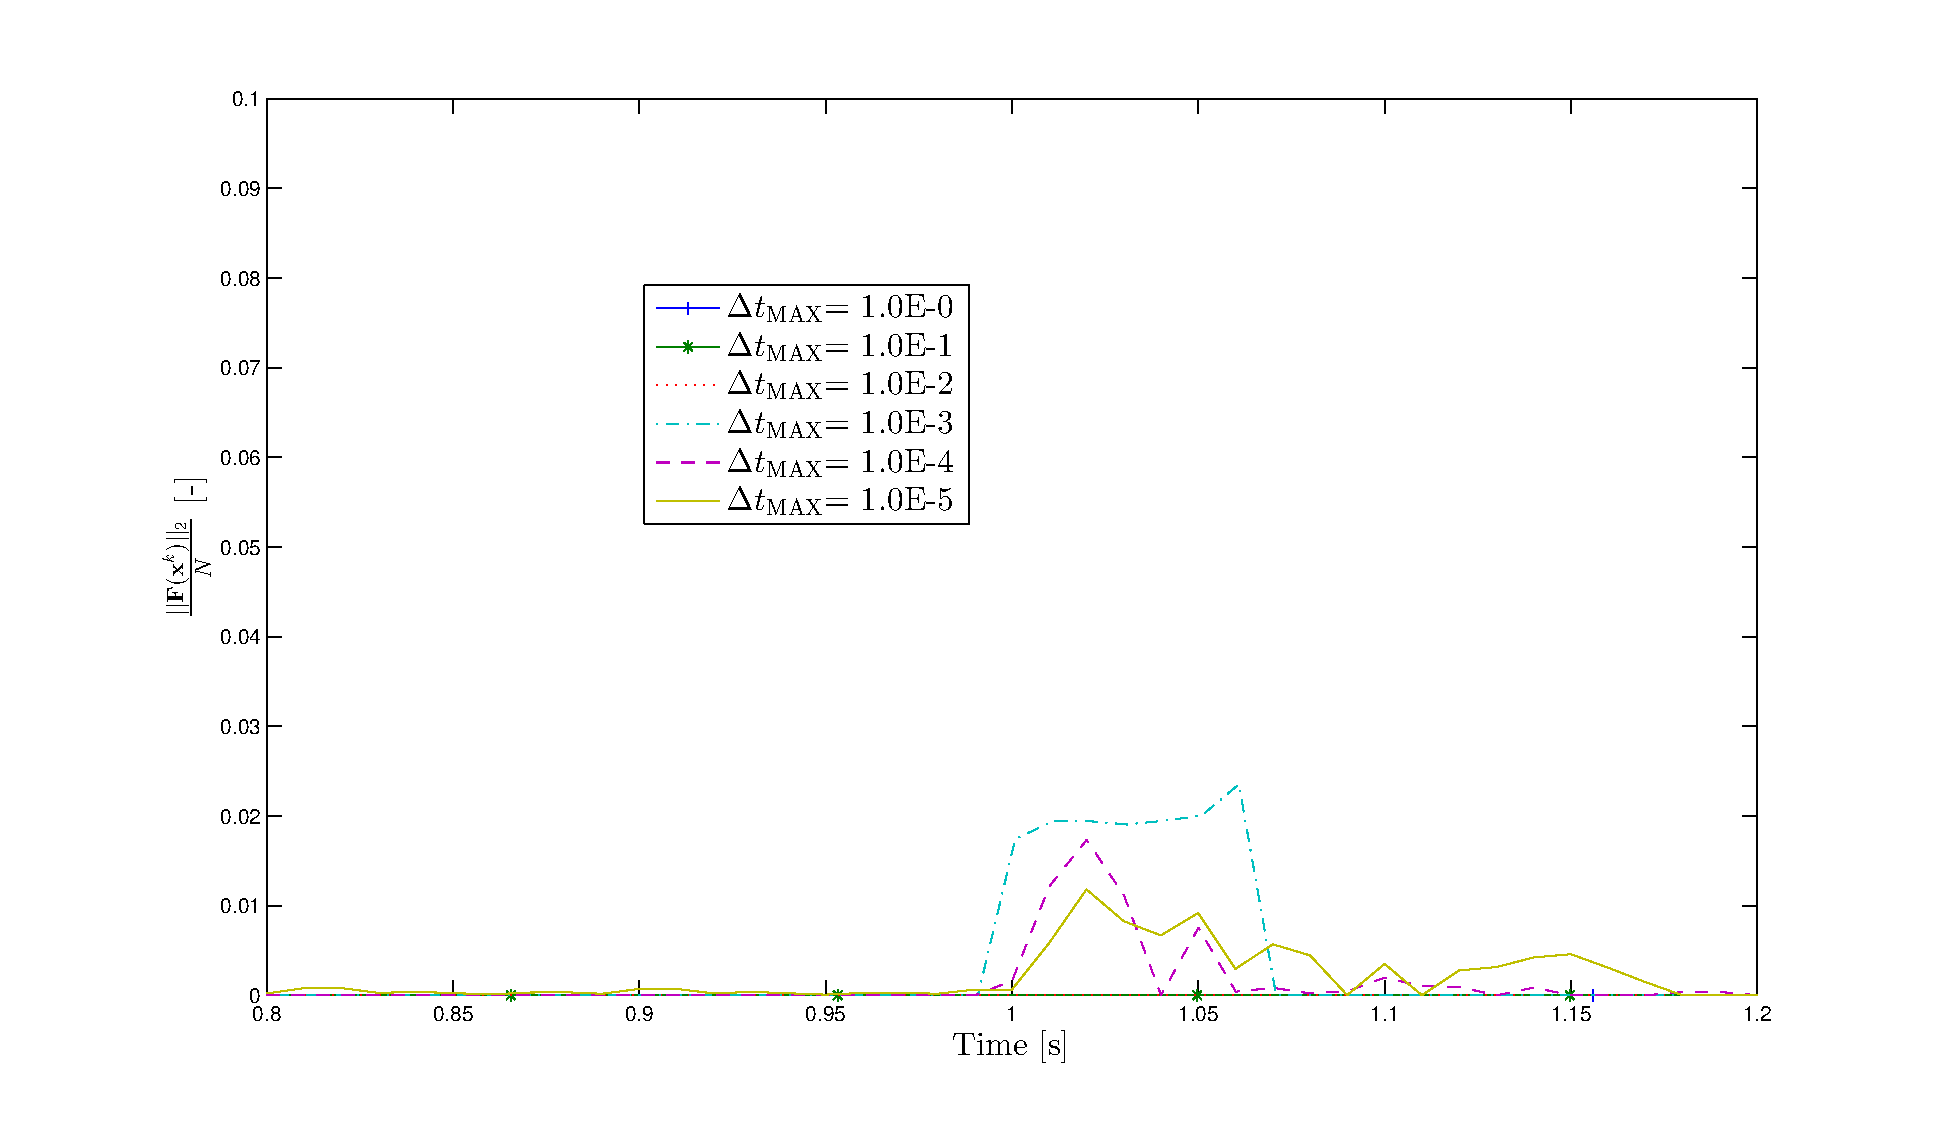
\includegraphics[width=0.49\textwidth]{images/nl_res_single_zoom.eps}
%\caption{Nonlinear mode solution residual for single-phase problem.}
%\label{fig:nl_res_single_zoom}
%\end{figure}

\begin{figure}[h!t]
\centering
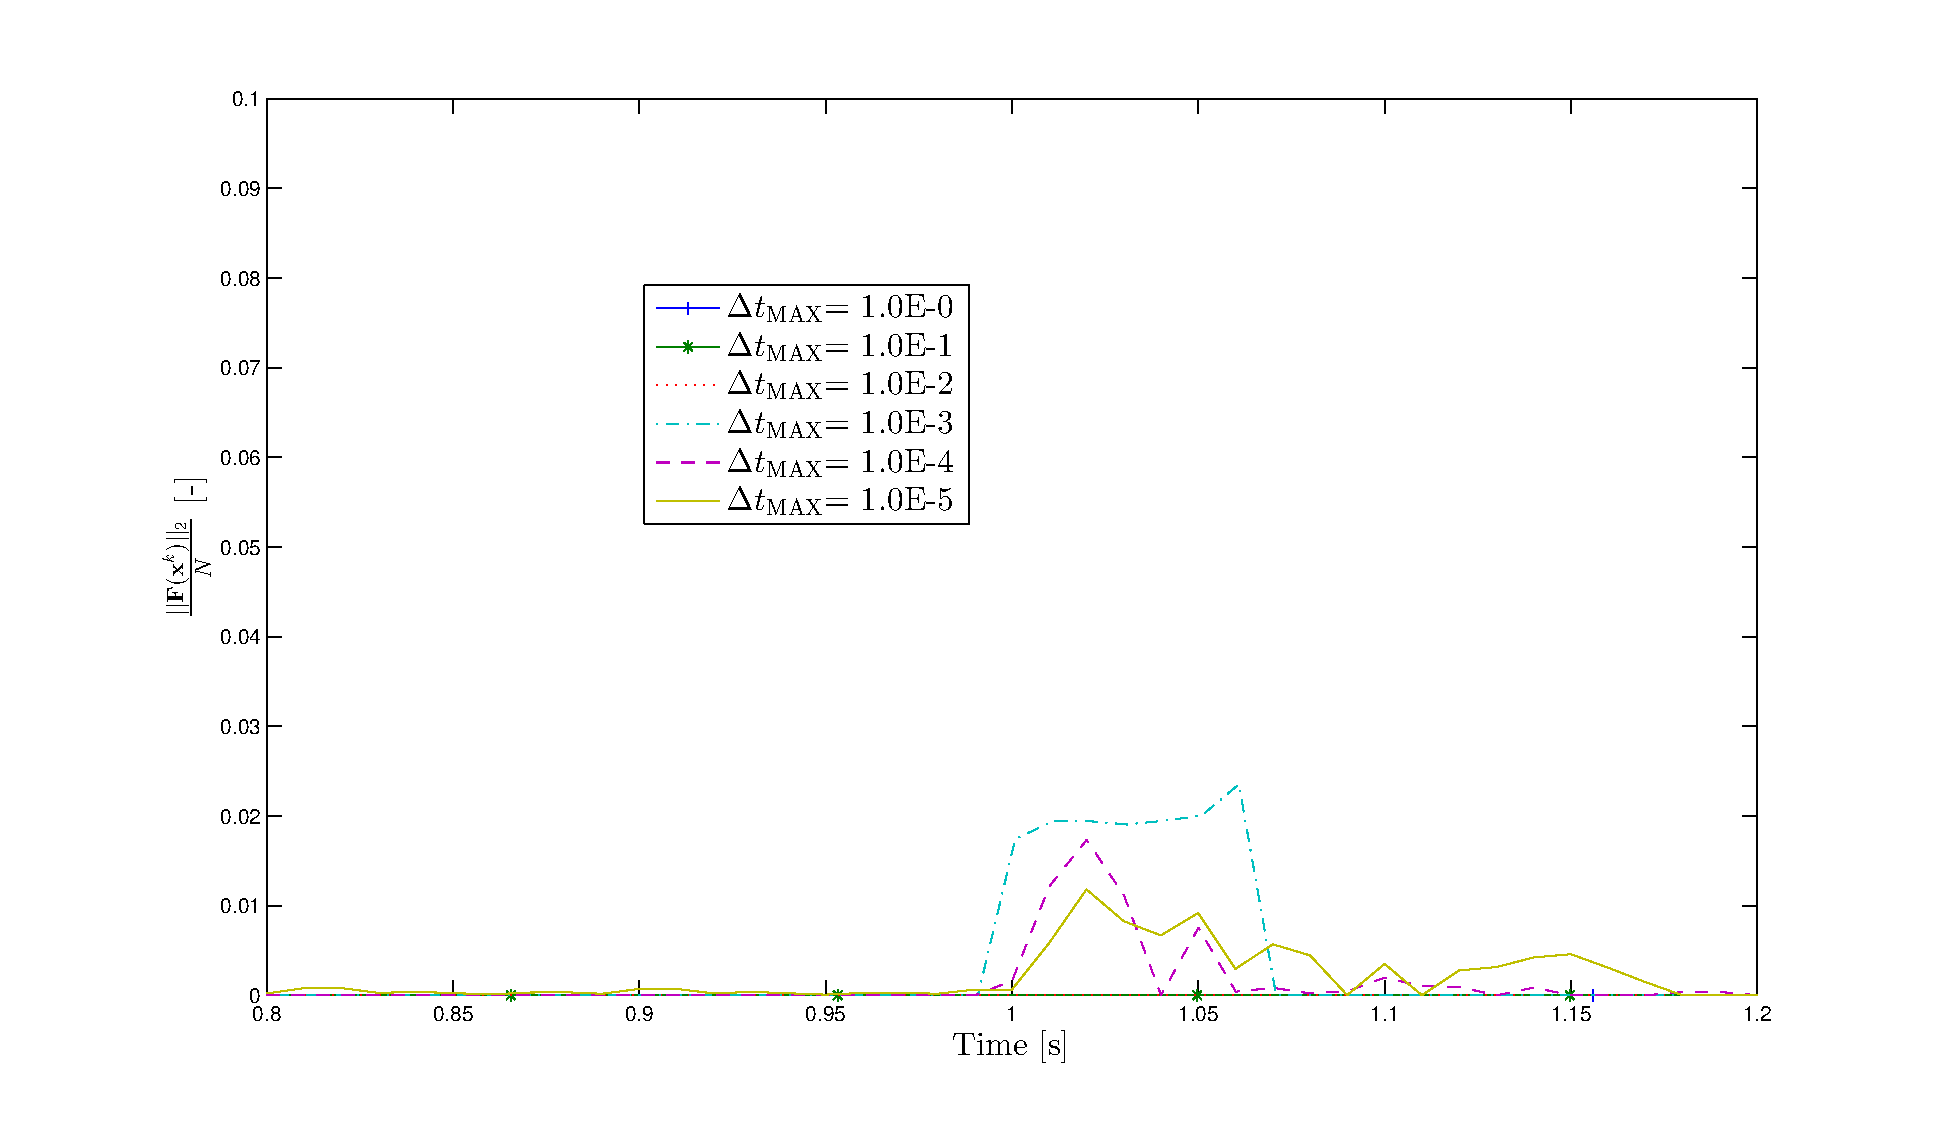
\includegraphics[width=0.94\textwidth]{images/nl_res_single_zoom.eps}
\caption{Zoomed residuals for the single-phase solution from the nonlinear solver.}
\label{fig:nl_res_single_zoom}
\end{figure}

This difference is manifested in the residuals for the nonlinear solver solution around 1 [s], \fig{fig:nl_res_single_zoom}.
The residual at the time of inlet flow initialization has a marked increase between the \dtmax{} = 1.0E-3 and \dtmax{} = 1.0E-2 solutions.
The reason for this behavior is, as of yet, unknown.
It is likely related to the same nonlinear non-convergence behavior remarked upon for the flashing problem. 

One way to quantify the difference between the solutions is by measuring the residual convergence metrics outlined in \sect{sect:temporal_convergence}.
These metrics provide a measure of how poorly the discrete nonlinear equations are being solved at every timestep in the transient.
The resolution of the residual allows for a solution that is less sensitive to timestep size selection than for a solution that does not resolve the residual.
The convergence metrics will be used to determine if a qualitative temporal-convergence determination can lead to the acceptance of a solution that is not nonlinearly converged.

For each of the test cases, the two different metrics were compared at the different \dtmax{}.
To examine efficacy of the the temporal convergence criteria, both the average and moment based temporal convergence criteria were evaluated for each of the twenty-three successful simulations.
The values of these metrics will be compared between different solvers for the same test problem. 

The two different nonlinear convergence metrics will now be examined for the flashing problem.
\tab{tab:flashing_criteria} shows both the average metric, $\tilde{R}$, and the moment based metric, $\tilde{R}_{\text{M}}$.
The entry for the legacy mode solution at 1 [s] is empty, reflecting its inability to solve the problem.
For the nonlinear solver, both metrics are decreasing as the \dtmax{} is decreased.
While the legacy solver also shows a decreasing residual metric, it does not decrease in order-of-magnitude, indicating that as the \dtmax{} is reduced the nonlinearities in the problem are not being sufficiently resolved.

\begin{table}[h!t]
\centering
\begin{tabular}{@{}l r@{.}l r@{.}l r@{.}l r@{.}l @{}}
\toprule
& \multicolumn{4}{c}{$\tilde{R}$} & \multicolumn{4}{c}{$\tilde{R}_{\text{M}}$}  \\
$\dtmax{}$ & \multicolumn{2}{c}{Legacy} & \multicolumn{2}{c}{Nonlinear} & \multicolumn{2}{c}{Legacy}& \multicolumn{2}{c}{Nonlinear}  \\
\midrule
1.0    & \multicolumn{2}{c}{-} & 1&177E-3 & \multicolumn{2}{c}{-} & 6&885E-4 \\
1.0E-1 & 5&487E-2 & 1&141E-3 & 5&044E-2 & 6&730E-4 \\
1.0E-2 & 4&960E-2 & 3&413E-4 & 4&570E-2 & 2&511E-4 \\
1.0E-3 & 3&172E-2 & 2&669E-4 & 2&372E-2 & 1&975E-4 \\
1.0E-4 & 2&504E-2 & 1&346E-4 & 1&838E-2 & 8&974E-5 \\
1.0E-5 & 2&166E-2 & 5&075E-5 & 1&922E-2 & 4&581E-5 \\
\bottomrule  
\end{tabular}
\caption{Nonlinear convergence metrics for flashing problem.}
\label{tab:flashing_criteria}
\end{table}

\begin{table}[h!t]
\centering
\begin{tabular}{@{}l r@{.}l r@{.}l r@{.}l r@{.}l @{}}
\toprule
& \multicolumn{4}{c}{$\tilde{R}$} & \multicolumn{4}{c}{$\tilde{R}_{\text{M}}$}  \\
$\dtmax{}$ & \multicolumn{2}{c}{Legacy} & \multicolumn{2}{c}{Nonlinear} & \multicolumn{2}{c}{Legacy}& \multicolumn{2}{c}{Nonlinear}  \\
\midrule
1.0    & 3&149E-3 & 1&700E-3 & 1&485E-3 & 1&070E-4 \\
1.0E-1 & 2&866E-3 & 1&700E-3 & 1&287E-3 & 1&070E-4 \\
1.0E-2 & 3&412E-4 & 1&357E-3 & 1&417E-4 & 7&701E-5 \\
1.0E-3 & 2&207E-4 & 4&584E-4 & 8&805E-5 & 1&178E-4 \\
1.0E-4 & 1&672E-4 & 1&588E-3 & 1&834E-5 & 4&958E-5 \\
1.0E-5 & 5&493E-4 & 2&758E-4 & 1&916E-5 & 8&939E-5 \\
\bottomrule  
\end{tabular}
\caption{Nonlinear convergence metrics for the single-phase problem.}
\label{tab:single_criteria}
\end{table}

\tab{tab:single_criteria} shows the two metrics for the single-phase problem.
Since the single-phase problem is relatively linear, the legacy solver produces metrics that are on the same order as those for the nonlinear solver.
Due to the non-convergence of the nonlinear solver at \dtmax{} = 1.0E-3, the moment based metric for the nonlinear solver is greater than the equivalent legacy solver metric.

\section{Review}
\label{sect:review}

In review, the single-shot semi-implicit \cobra{} software was converted to a nonlinearly convergent, semi-implicit algorithm.
An operator-based scaling was introduced and implemented into both the legacy and the nonlinear \cobra{} solvers.
The nonlinear solver produced results that were qualitatively different than those obtained from the legacy solver for the problem with high nonlinearities.
Tests indicated that a timestep size insensitive solution may not be nonlinearly converged.
It was shown that the nonlinear solver produces results that are indistinguishable from those produced by the legacy solver for the single-phase problem, which has relatively mild nonlinearities.
A deficiency was identified with the current implementation of the operator-based scaling.
The scaled residual had nontrivial values during the steady state initialization portion of both problems.
Additionally, a deficiency was detected with the convergence limits of the nonlinear solver.
A metric to quantify the nonlinear convergence of a timestep size insensitive simulation was developed and implemented.
This non-convergence of the discrete nonlinear system in the legacy solver mode produced a qualitatively different solution from the nonlinear solver.   % Chapter: Proof of worthiness. 
\chapter{Work Proposal}
\label{chap:proposal}
To evaluate the proposed method, several objectives will be pursued.
The coding of the operator based scaling for the nonlinear residuals will be examined and modified as necessary to address the noted convergence issues.
An appropriate scaling of the Newton updates for convergence testing both within the linesearch algorithm and in the Newton loop will be determined.
The domain decomposition algorithm will be mathematically developed, coded, and evaluated.
Once the preceding three objectives have been met, a test problem will be developed to test the nonlinear refinement code as applied to a predetermined subdomain.
After the algorithmic framework has been evaluated, several geometrically complex problems with high local-nonlinearities will be developed to obtain temporal-convergence benchmarks of the legacy algorithm.
The same problems will then be evaluated using the proposed algorithm to determine the efficacy of temporal-convergence criteria.
Upon completion of the temporal-convergence tests, run time tests will be conducted to determine any performance gains or losses as a result of the proposed method.
Parametric studies will then be conducted to determine the impact of nonlinear convergence tolerances, phase appearance and disappearance thresholds, geometric residual imbalances, and residual thresholds for activation of nonlinear refinements.

\section{Scaling Evaluation}
\label{sect:proposal_scaling}
The current implementation of the physics based scaling method outlined in \sect{sect:operator_scaling} has several issues that need to be addressed.
Another scaling question that needs to be addressed is the proper scaling for the newton update.

\section{Domain Decomposition}
\label{sect:domain_coupling}
The first step will be to implement a variation of the semi-implicit domain coupling algorithm presented in \sect{sect:code_coupling}.
The details of the derivation will need to be reworked to account for the different flow variables.

Upon completion of the implementation, a rigorous testing of the coupling method will be conducted.
This testing will be similar to that conducted by \citet{Weaver2002}.

\section{Temporal-Convergence Testing and Bench-marking}
\label{sect:proposal_temporal_testing}
To evaluate the domain decomposition capabilities, a geometric test problem will need to be developed.
This problem should have a singular characteristic: multiple geometric components.
The problem will be a single phase run
The test problem will be run in legacy mode to obtain a standard solution.

\section{Performance Evaluation}
\label{sect:proposal_performance_evaluation}
Upon completion 

\section{Parametric Studies}
\label{sect:proposal_parametric_studies}
Given the wide range of parameters

\section{Time Line}
\label{sect:proposal_time_line}


\fig{fig:time_line}

\begin{figure}[ht]
\caption{Proposed test matrix.}
\label{fig:time_line}
\begin{center}
Picture goes here.
\end{center}
\end{figure}

      % Chapter: Proposal of research.

%=======================================================================
% Bibliography
%=======================================================================
\bibliographystyle{plainnat}
\bibliography{../references/references}

%=======================================================================
% Appendices
%=======================================================================
\begin{appendices}

\chapter{COBRA-IE Input Decks}
\label{app:input_decks}

\section{Single Phase Input Deck}
%\singlespace
%{\tiny \verbatiminput{input_decks/single.tex}}

%\pagebreak
\section{Flashing Input Deck}
%{\tiny \verbatiminput{input_decks/flashing.tex}}

%\pagebreak
\section{GE Mixing 2B3-2 Input Deck}
%{\tiny \verbatiminput{input_decks/mixing.tex}}

%\pagebreak
\section{Quench Type Problem Input Deck}
%{\small \verbatiminput{input_decks/quench.inp}}

%\pagebreak
\section{Valve Type Problem Input Deck}
%{\small \verbatiminput{input_decks/valve.inp}}         % Appendix: Input Decks
%\chapter{Discrete Conservation Equations}
\label{app:residuals}

\section{Continuity Equations}

\subsection{Mass}

\begin{IEEEeqnarray}{lCr}
 \frac{\partial}{\partial t} \alpha_g \rho_g + \nabla\cdot\left(\alpha_g\rho_g\vec{U}_g\right) & = & \Gamma''' \\
 \frac{\partial}{\partial t} \alpha_l \rho_l + \nabla\cdot\left(\alpha_l\rho_l\vec{U}_l\right) & = & -(1-\eta) \Gamma''' - S''' \\
 \frac{\partial}{\partial t} \alpha_e \rho_l + \nabla\cdot\left(\alpha_e\rho_l\vec{U}_e\right) & = & -\eta \Gamma''' + S'''\\
 \frac{\partial}{\partial t} \alpha_g \rho_{nc} + \nabla\cdot\left(\alpha_g\rho_{nc}\vec{U}_g\right) & = & \Gamma''' 
 \end{IEEEeqnarray}

\begin{IEEEeqnarray}{lCl}
 % Here is the vapor mass equation.
 (\alpha \rho_v)^{n+1} + \frac{\Delta t}{V_c}\left[\sum_{J} \left[\frac{(\alpha \rho_{v})^{*}}{<\alpha \rho_v>}\right]^{n} \dot{\vec{M}}^{n+1}_{v}\cdot \vec{\hat{n}} + \sum_{K} \left[\frac{(\alpha \rho_{v})^{*}}{<\alpha \rho_v>}\right]^{n} \dot{\vec{W}}^{n+1}_{v}\cdot \vec{\hat{n}}\right] & & \nonumber \\
 = (\alpha \rho_v)^{n} + \frac{\Delta t}{V_c} \Gamma^{\,n+1} & & \\
 % Here is the gas mass equation.
 (\alpha \rho_g)^{n+1} + \frac{\Delta t}{V_c}\left[\sum_{J} \left[\frac{(\alpha \rho_{g})^{*}}{<\alpha \rho_g>}\right]^{n} \dot{\vec{M}}^{n+1}_{v}\cdot \vec{\hat{n}} + \sum_{K} \left[\frac{(\alpha \rho_{g})^{*}}{<\alpha \rho_g>}\right]^{n} \dot{\vec{W}}^{n+1}_{v}\cdot \vec{\hat{n}}\right] & & \nonumber \\
 = (\alpha \rho_g)^{n} & &  \\
 % Here is the continuous liquid mass equation.
 (\alpha_l \rho_l)^{n+1} + \frac{\Delta t}{V_c}\left[\sum_{J} \left[\frac{(\alpha_l \rho_{l})^{*}}{<\alpha_l \rho_l>}\right]^{n} \dot{\vec{M}}^{n+1}_{l}\cdot \vec{\hat{n}} + \sum_{K} \left[\frac{(\alpha_l \rho_{l})^{*}}{<\alpha_l \rho_l>}\right]^{n} \dot{\vec{W}}^{n+1}_{l}\cdot \vec{\hat{n}}\right] & & \nonumber \\
 = (\alpha_l \rho_l)^{n} + \frac{\Delta t}{V_c} \left(S_{D}^{n+1} - (1-\eta^{n})\Gamma^{\,n+1}_{l} - S_{E}^{n+1}\right) & & \\
 % Here is the entrained liquid mass equation.
 (\alpha_e \rho_l)^{n+1} + \frac{\Delta t}{V_c}\left[\sum_{J} \left[\frac{(\alpha_e \rho_{l})^{*}}{<\alpha_e \rho_l>}\right]^{n} \dot{\vec{M}}^{n+1}_{e}\cdot \vec{\hat{n}} + \sum_{K} \left[\frac{(\alpha_e \rho_{l})^{*}}{<\alpha_e \rho_l>}\right]^{n} \dot{\vec{W}}^{n+1}_{e}\cdot \vec{\hat{n}}\right] & & \nonumber \\
 = (\alpha_e \rho_l)^{n} + \frac{\Delta t}{V_c} \left(S_{E}^{n+1} - \eta^{n}\Gamma^{\,n+1}_{e} - S_{D}^{n+1}\right)& & 
 \end{IEEEeqnarray}

\subsection{Energy}

\begin{IEEEeqnarray}{Cr}
 \frac{\partial}{\partial t}\left(\alpha_g (\rho_v h_v+\rho_{nc} h_{nc})\right)+\nabla\cdot\left(\alpha_g(\rho_v h_v + \rho_{nc} h_{nc}) \vec{U}_g\right) & \nonumber \\
 = \Gamma'''h'_{v} + q'''_{i,v} + q'''_{gl} + q'''_{wg} + \alpha_g \frac{\partial P}{\partial t} & \\
 \frac{\partial}{\partial t}\left((\alpha_e +\alpha_l) \rho_l h_l\right)+\nabla\cdot\left(\alpha_l\rho_l h_l \vec{U}_l\right)+\nabla\cdot\left(\alpha_e\rho_l h_l \vec{U}_e\right)  \nonumber \\
 = \Gamma'''h'_{v} + q'''_{i,v} + q'''_{gl} + q'''_{wg} + \alpha_g \frac{\partial P}{\partial t} &
 \end{IEEEeqnarray}

\begin{IEEEeqnarray}{ll}
 % Here be the gas equations.
  & (\alpha_g (\rho_v h_v + \rho_{nc} h_{nc}) )^{n+1} - \alpha_{g}^{n}P^{\;n+1} \nonumber \\
 +& \frac{\Delta t}{V_c} \sum_{J} \left(\frac{(\alpha_g (\rho_v h_v + \rho_{nc} h_{nc}) )^{*}}{<\alpha_g (\rho_v h_v + \rho_{nc} h_{nc}) >}\right)^{n} \dot{\vec{M}}^{n+1}_{v}\cdot \vec{\hat{n}} \nonumber \\
 +& \frac{\Delta t}{V_c} \sum_{K} \left(\frac{(\alpha_g (\rho_v h_v + \rho_{nc} h_{nc}) )^{*}}{<\alpha_g (\rho_v h_v + \rho_{nc} h_{nc}) >}\right)^{n} \dot{\vec{W}}^{n+1}_{v}\cdot \vec{\hat{n}} \nonumber \\
 =& (\alpha_g (\rho_v h_v + \rho_{nc} h_{nc}) )^{n} - \alpha_{g}^{n}P^{\;n} + \frac{\Delta t}{V_c}\left(q^{n}_{wg} + q^{n}_{i,v} + \Gamma^{\,n}h'^{\,n}_{v} + q^{n}_{gl}\right)\\
 % Here be the liquid equations.
  & ((\alpha_e +\alpha_l) \rho_l h_l)^{n+1} - (\alpha_e +\alpha_l)^{n}P^{\;n+1} \nonumber \\
 +& \frac{\Delta t}{V_c} \sum_{J}\left[  \left(\frac{(\alpha_l \rho_l h_l )^{*}}{<\alpha_l \rho_l h_l >}\right)^{n} \dot{\vec{M}}^{n+1}_{l}\cdot \vec{\hat{n}}+ \left(\frac{(\alpha_e \rho_l h_l )^{*}}{<\alpha_e \rho_l h_l >}\right)^{n} \dot{\vec{M}}^{n+1}_{e}\cdot \vec{\hat{n}}\right] \nonumber \\
 +& \frac{\Delta t}{V_c} \sum_{K}\left[  \left(\frac{(\alpha_l \rho_l h_l )^{*}}{<\alpha_l \rho_l h_l >}\right)^{n} \dot{\vec{W}}^{n+1}_{l}\cdot \vec{\hat{n}}+ \left(\frac{(\alpha_e \rho_l h_l )^{*}}{<\alpha_e \rho_l h_l >}\right)^{n} \dot{\vec{W}}^{n+1}_{e}\cdot \vec{\hat{n}}\right] \nonumber \\
 =& ((\alpha_e +\alpha_l) \rho_l h_l)^{n} - (\alpha_e +\alpha_l)^{n}P^{\;n} + \frac{\Delta t}{V_c}\left(q^{n}_{wl} + q^{n}_{i,l} -\Gamma^{\,n}h'^{\,n}_{l} - q^{n}_{gl}\right)
 \end{IEEEeqnarray}

 \begin{IEEEeqnarray}{lr}
 \frac{\partial }{\partial t} \left(\alpha_g (\rho_v + \rho_{nc}) \Vec{U}_g \right) + \nabla\cdot\left(\alpha_g (\rho_v + \rho_{nc}) \vec{U}_g \vec{U}_g \right) = &\nonumber \\
 -\alpha_g\;\nabla P + \alpha_g (\rho_v + \rho_{nc}) \vec{g} - \tau^{'}_{wg}-\tau^{'}_{I_{gl}} - \tau^{'}_{I_{ge}} + \Gamma''' \vec{U}^{'} & \\
 \frac{\partial }{\partial t} \left(\alpha_l \rho_l \Vec{U}_l \right) + \nabla\cdot\left(\alpha_l \rho_l \vec{U}_l \vec{U}_l \right) = &\nonumber \\
 -\alpha_l\;\nabla P + \alpha_l \rho_l \vec{g} - \tau^{'}_{wl} + \tau^{'}_{I_{gl}} -\left((1-\eta)\Gamma'''\vec{U}'\right) - S'''\vec{U}'& \\
 \frac{\partial }{\partial t} \left(\alpha_e \rho_l \Vec{U}_e \right) + \nabla\cdot\left(\alpha_e \rho_l \vec{U}_e \vec{U}_e \right) = &\nonumber \\
 -\alpha_e\;\nabla P + \alpha_e \rho_l \vec{g} - \tau^{'}_{wl} + \tau^{'}_{I_{ge}} -\left(\eta\Gamma'''\vec{U}'\right) + S'''\vec{U}'&
 \end{IEEEeqnarray}

 \begin{IEEEeqnarray}{rCl}
 F_g(\Vec{x}^{n+1}) & = & \overbrace{E_g({\Vec{x}^{n}})}^{\text{Purely explicit terms}}-\overbrace{A_{mom,j}\Delta z_j\left[ \alpha_g^n\frac{P_{J+1}^{n+1}-P_{J}^{n+1}}{\Delta z_j}\right]}^{\text{Semi-Implicit Pressure Term}}  \\
 & - & \overbrace{A_{mom,j}\Delta z_j\left[ \frac{dP}{dz}\bigg|_{w,g}^{*}+\frac{dP}{dz}\bigg|_{i,lg}^{*}+\frac{dP}{dz}\bigg|_{i,eg}^{*}\right]}^{\text{Semi-Implicit Drag Terms}}\nonumber \\
 & + & \overbrace{\mathcal{S}p^{n+1}_{g,j}}^{\text{Implicit Source Term}} -\overbrace{\frac{\left(M_{g,j}^{n+1}-M_{g,j}^{n}\right)}{\Delta t}\Delta z}^{\text{Time rate of change}}\nonumber \\
 & = &  0 \nonumber
 \end{IEEEeqnarray}  % Appendix: Nonlinear Math
%\chapter{Two-phase Flow Equations}
\label{app:two_phase_flow}

Two phase flow is crazy.

\section{blarger}
\label{sect:blarger}
The details of two phase flow are given here.

      % Appendix: Two Phase Flow
%\chapter{Newton Steps}
\label{app:newton}

 Linearization of the axial momentum equations in COBRA-IE.

\begin{IEEEeqnarray}{rCl}
  \vec{x}_k & = \begin{bmatrix}
   \dot{\vec{M}}_k \\
   \Delta \text{P}_k
 \end{bmatrix}\ & = \begin{bmatrix}
 \dot{M}_{l,k}\\
 \dot{M}_{g,k}\\
 \dot{M}_{e,k}\\
 \Delta \text{P}_{k}
 \end{bmatrix}
 \end{IEEEeqnarray}

 Note: 

 \begin{IEEEeqnarray}{rCCCr}
 \vec{L}(\vec{x}_{k}) & = & \mat{L}\;\dot{\vec{M}}_{k} + \vec{b}\Delta\text{P}_{k} \nonumber \\
 \frac{\partial}{\partial \Delta\text{P}_{k}}\left[\vec{b} \Delta \text{P}_{k}\right] & = & \vec{b} \nonumber \\
 \frac{\partial\; \vec{N}(\vec{x}_{k})}{\partial \vec{x}_{k}} & = & \frac{\partial\; \vec{N}(\vec{x}_{k})}{\partial \dot{\vec{M}}_{k}} & = & \mat{N}(\dot{\vec{M}}_{k}) \nonumber \\
 \mat{J}^{*}_{k} & = & \frac{\partial\; \vec{F}(\vec{x}_{k})}{\partial \dot{\vec{M}_{k}}} & = & \mat{L} + \mat{N}(\dot{\vec{M}}_{k})  \nonumber \\
 \mat{J}_{\,k}\delta \vec{x} & = & \frac{\partial\; \vec{F}(\vec{x}_{k})}{\partial \vec{x}_{k}}\delta\vec{x} & = & \mat{J}^{*}_{\,k}\delta(\dot{\vec{M}}) + \vec{b}\delta(\Delta \text{P})\nonumber
 \end{IEEEeqnarray}



Current View Point

\begin{IEEEeqnarray}{rCl}
 0 & = & \vec{F}(\vec{x}_{k+1}) \nonumber \\
 0 & = & \vec{F}(\vec{x}_{k+1}) =  \vec{E} + \vec{L}(\vec{x}_{k+1}) + \vec{N}(\vec{x}_{k+1})  \nonumber \\
 0 & = & \vec{E} + \vec{L}(\vec{x}_{k+1}) + \vec{N}(\vec{x}_{k+1}) \nonumber \\
 0 & = & \vec{E} + \mat{L}\;\dot{\vec{M}}_{k+1} + \vec{b}\Delta\text{P}_{k+1} + \vec{N}(\vec{x}_{k+1}) \nonumber \\
 0 & = & \vec{E} + \mat{L}\;\dot{\vec{M}}_{k+1} + \vec{b}\Delta \text{P}_{k} + \frac{\partial\left[ \vec{b}\Delta\text{P}_{k+1}\right]}{\partial\,\Delta \text{P}_{k+1}}\delta(\Delta \text{P}) + \vec{N}(\vec{x}_{k}) + \frac{\partial \left[ \vec{N}(\vec{x}_{k+1})\right]}{\partial\, \vec{x}_{k+1}}\left[\vec{x}_{k+1}-\vec{x}_{k}\right] \nonumber
 \end{IEEEeqnarray}

 \begin{IEEEeqnarray}{rCl}
  \mat{L}\;\dot{\vec{M}}_{k+1} + \mat{N}(\dot{\vec{M}}_{k})\;\dot{\vec{M}}_{k+1} & = & -\vec{E} - \vec{b}\Delta \text{P}_{k} - \vec{N}(\vec{x}_{k}) - \vec{b}\delta(\Delta \text{P}) + \mat{N}(\dot{\vec{M}}_{k})\dot{\vec{M}}_{k} \nonumber \\
  \left[\mat{L} + \mat{N}(\dot{\vec{M}}_{k})\right]\dot{\vec{M}}_{k+1} & = & - \left[\vec{E} + \vec{b}\Delta \text{P}_{k} + \vec{N}(\vec{x}_{k}) - \mat{N}(\dot{\vec{M}}_{k})\;\dot{\vec{M}}_{k}\right] - \vec{b}\delta(\Delta \text{P}) \nonumber \\
  \mat{J}^{*}_{\,k}\; \dot{\vec{M}}_{k+1} & = &  -\vec{f} - \vec{b}\delta(\Delta \text{P}) \nonumber \\
 \dot{\vec{M}}_{k+1} & = &  \underbrace{-\mat{J}_{\,k}^{-*}\;\vec{f}}_{\dot{\vec{M}}^{\widetilde{n+1}}_{\,k}} \underbrace{- \mat{J}^{-*}_{\,k}\;\vec{b}}_{\frac{d \dot{\vec{M}}_{k}}{d \Delta \text{P}}}\delta(\Delta \text{P}) \nonumber \\
 \dot{\vec{M}}_{k+1} & = &  \dot{\vec{M}}^{\widetilde{n+1}}_{\,k} + \frac{d \dot{\vec{M}}_{k}}{d \Delta \text{P}}\delta(\Delta \text{P}) \nonumber 
 \end{IEEEeqnarray}

Relation between Newton step and current formulation.

 \begin{IEEEeqnarray}{rCl}
 \left[\mat{L} + \mat{N}(\dot{\vec{M}}_{k})\right]\dot{\vec{M}}_{k+1} & = & - \left[\vec{E} + \mat{L}\;\dot{\vec{M}}_{k} + \vec{b}\Delta \text{P}_{k} + \vec{N}(\vec{x}_{k}) \right] \nonumber \\
 & & - \vec{b}\delta(\Delta \text{P}) + \mat{L}\;\dot{\vec{M}}_{k} + \mat{N}(\dot{\vec{M}}_{k})\;\dot{\vec{M}}_{k} \nonumber \\
 \left[\mat{L} + \mat{N}(\dot{\vec{M}}_{k})\right]\dot{\vec{M}}_{k+1} & = & - \vec{F}(\vec{x}_{k}) - \vec{b}\delta(\Delta \text{P}) + \left[\mat{L} + \mat{N}(\dot{\vec{M}}_{k})\right]\;\dot{\vec{M}}_{k} \nonumber \\
 \mat{J}^{*}_{\,k}\,\dot{\vec{M}}_{k+1} & = & - \vec{F}(\vec{x}_{k}) - \vec{b}\delta(\Delta \text{P}) + \mat{J}^{*}_{\,k}\;\dot{\vec{M}}_{k} \nonumber \\
 \dot{\vec{M}}_{k+1} & = & \underbrace{\dot{\vec{M}}_{k} - \mat{J}_{\,k}^{-*} \vec{F}(\vec{x}_{k})}_{\dot{\vec{M}}^{\widetilde{n+1}}_{\,k}} \underbrace{- \mat{J}_{\,k}^{-1}\vec{b}}_{\frac{d \dot{\vec{M}}_{k}}{d \Delta \text{P}}}\delta\text{P} \nonumber \\
 \dot{\vec{M}}_{k+1} & = &  \dot{\vec{M}}^{\widetilde{n+1}}_{\,k} + \frac{d \dot{\vec{M}}_{k}}{d \Delta \text{P}}\delta(\Delta \text{P}) \nonumber 
 \end{IEEEeqnarray}


Equivalence with a Newton step.

 \begin{IEEEeqnarray}{rCl}
 \left[\mat{L} + \mat{N}(\dot{\vec{M}}_{k})\right]\dot{\vec{M}}_{k+1} & = & - \left[\vec{E} + \mat{L}\;\dot{\vec{M}}_{k} + \vec{b}\Delta \text{P}_{k} + \vec{N}(\vec{x}_{k}) \right] \nonumber \\
 & & - \vec{b}\delta(\Delta \text{P}) + \mat{L}\;\dot{\vec{M}}_{k} + \mat{N}(\dot{\vec{M}}_{k})\;\dot{\vec{M}}_{k} \nonumber \\
 \left[\mat{L} + \mat{N}(\dot{\vec{M}}_{k})\right]\dot{\vec{M}}_{k+1} & = & - \vec{F}(\vec{x}_{k}) - \vec{b}\delta(\Delta \text{P}) + \left[\mat{L} + \mat{N}(\dot{\vec{M}}_{k})\right]\;\dot{\vec{M}}_{k} \nonumber \\
 \mat{J}^{*}_{\,k}\,\dot{\vec{M}}_{k+1} & = & - \vec{F}(\vec{x}_{k}) - \vec{b}\delta(\Delta \text{P}) + \mat{J}^{*}_{\,k}\;\dot{\vec{M}}_{k} \nonumber \\
 \mat{J}^{*}_{\,k}\,\left[\dot{\vec{M}}_{k+1}-\dot{\vec{M}}_{k} \right] & = & - \vec{F}(\vec{x}_{k}) - \vec{b}\delta(\Delta \text{P}) \nonumber \\
 \mat{J}^{*}_{\,k}\,\delta(\dot{\vec{M}}) + \vec{b}\delta(\Delta \text{P})  & = & - \vec{F}(\vec{x}_{k})  \nonumber \\
 \mat{J}_{\,k}\,\delta\vec{x} + \vec{b}\delta(\Delta \text{P})  & = & - \vec{F}(\vec{x}_{k})  \nonumber 
 \end{IEEEeqnarray}

 \begin{align}
 \begin{bmatrix} 
 \DerivParOne{\vec{I}_{l}}{\vec{\dot{M}}_{l}} & \DerivParOne{\vec{I}_{l}}{\vec{\dot{M}}_{g}}  & \DerivParOne{\vec{I}_{l}}{\vec{\dot{M}}_{e}} & \DerivParOne{\vec{I}_{l}}{\Delta P}\\
 \DerivParOne{\vec{I}_{g}}{\vec{\dot{M}}_{l}} & \DerivParOne{\vec{I}_{g}}{\vec{\dot{M}}_{g}}  & \DerivParOne{\vec{I}_{g}}{\vec{\dot{M}}_{e}} & \DerivParOne{\vec{I}_{g}}{\Delta P}\\
 \DerivParOne{\vec{I}_{e}}{\vec{\dot{M}}_{l}} & \DerivParOne{\vec{I}_{e}}{\vec{\dot{M}}_{g}}  & \DerivParOne{\vec{I}_{e}}{\vec{\dot{M}}_{e}} & \DerivParOne{\vec{I}_{e}}{\Delta P}
 \end{bmatrix}_{0}
 \cdot
 \begin{bmatrix}
 \Delta \vec{\dot{M}}_l \\
 \Delta \vec{\dot{M}}_g \\
 \Delta \vec{\dot{M}}_e \\
 \Delta P
 \end{bmatrix}_{k\rightarrow k+1} & =
 -\begin{bmatrix}
 \vec{E}_{l} \\
 \vec{E}_{g} \\
 \vec{E}_{e}
 \end{bmatrix} -
 \begin{bmatrix}
 \vec{I}_{l} \\
 \vec{I}_{g} \\
 \vec{I}_{e}
 \end{bmatrix}_{k} \\ 
 % HERE IS A SEPERATE EQUATION
 \begin{bmatrix} 
 \DerivParOne{\vec{I}_{l}}{\vec{\dot{M}}_{l}} & \DerivParOne{\vec{I}_{l}}{\vec{\dot{M}}_{g}}  & \DerivParOne{\vec{I}_{l}}{\vec{\dot{M}}_{e}} \\
 \DerivParOne{\vec{I}_{g}}{\vec{\dot{M}}_{l}} & \DerivParOne{\vec{I}_{g}}{\vec{\dot{M}}_{g}}  & \DerivParOne{\vec{I}_{g}}{\vec{\dot{M}}_{e}} \\
 \DerivParOne{\vec{I}_{e}}{\vec{\dot{M}}_{l}} & \DerivParOne{\vec{I}_{e}}{\vec{\dot{M}}_{g}}  & \DerivParOne{\vec{I}_{e}}{\vec{\dot{M}}_{e}}
 \end{bmatrix}_{0}
 \cdot
 \begin{bmatrix}
 \Delta \vec{\dot{M}}_l \\
 \Delta \vec{\dot{M}}_g \\
 \Delta \vec{\dot{M}}_e
 \end{bmatrix}_{k\rightarrow k+1} & =
 -\vec{E} -
 \vec{I}_{k} -
 \begin{bmatrix}
 \DerivParOne{\vec{I}_{l}}{\Delta P} \\
 \DerivParOne{\vec{I}_{g}}{\Delta P} \\
 \DerivParOne{\vec{I}_{e}}{\Delta P}
 \end{bmatrix}_{0}
 \Delta P_{k \rightarrow k+1} \\
 % HERE IS A SEPERATE EQUATION
 \mat{J}_{\,0}
 \cdot
 \begin{bmatrix}
 \Delta \vec{\dot{M}}_l \\
 \Delta \vec{\dot{M}}_g \\
 \Delta \vec{\dot{M}}_e
 \end{bmatrix}_{k\rightarrow k+1} & =
 -\vec{E} -
 \vec{I}_{k} -
 \vec{p}_{0}
 \Delta P_{k \rightarrow k+1} \\
 % HERE IS A SEPERATE EQUATION
 \begin{bmatrix}
 \Delta \vec{\dot{M}}_l \\
 \Delta \vec{\dot{M}}_g \\
 \Delta \vec{\dot{M}}_e
 \end{bmatrix}_{k\rightarrow k+1} & =
 -\mat{J}_{\,0}^{-1}\left(\vec{E} + \vec{I}_{k}\right) -
 \mat{J}_{\,0}^{-1} \cdot \vec{p}_{0} \Delta P_{k \rightarrow k+1} 
  \end{align}
  \begin{align}
 % HERE IS A SEPERATE EQUATION
 \vec{\dot{M}}^{n+1}_{k+1}- \vec{\dot{M}}^{n+1}_{k} & =
 -\mat{J}_{\,0}^{-1}\left(\vec{E} + \vec{I}_{k}\right) -
 \mat{J}_{\,0}^{-1} \cdot \vec{p}_{0} \Delta P_{k \rightarrow k+1}\\
 % HERE IS A SEPERATE EQUATION
 \vec{\dot{M}}^{n+1}_{k+1} & =
 \underbrace{\vec{\dot{M}}^{n+1}_{k} -\mat{J}_{\,0}^{-1}\left(\vec{E} + \vec{I}_{k}\right)}_{\vec{\dot{M}}^{*}_{k}} - \underbrace{\mat{J}_{\,0}^{-1} \cdot \vec{p}_{0}}_{\frac{\partial \vec{\dot{M}}}{\partial \Delta P}} \Delta P_{k \rightarrow k+1} \\
 % HERE IS A SEPERATE EQUATION
 \vec{\dot{M}}^{n+1}_{k+1} & =
 \underbrace{-\mat{J}_{\,0}^{-1}\cdot \vec{E} + \vec{\dot{M}}^{n+1}_{k} - \mat{J}^{-1}_{\,0}\cdot \vec{I}_{k}}_{\vec{\dot{M}}^{n+1}_{*}} - \underbrace{\mat{J}_{\,0}^{-1} \cdot \vec{p}_{0}}_{\frac{\partial \vec{\dot{M}}}{\partial \Delta P}} \Delta P_{k \rightarrow k+1}
 \end{align}

 \begin{align}
 % HERE IS A SEPERATE EQUATION
 \vec{\dot{m}}^{n+1}_{k+1} & =
 \underbrace{-\mat{J}_{\,0}^{-1}\cdot \vec{E} + \vec{\dot{m}}^{n+1}_{k} - \mat{J}_{\,0}\cdot \vec{I}_{k}}_{\vec{\dot{m}}^{n+1}_{*}} - \underbrace{\mat{J}_{\,0}^{-1} \cdot \vec{p}_{0}}_{\frac{\partial \vec{\dot{m}}}{\partial \Delta P}} \Delta P_{k \rightarrow k+1} \\
 % HERE IS A SEPERATE EQUATION
 \vec{\dot{m}}^{n+1}_{k+1} & =
 \underbrace{-\mat{J}_{\,0}^{-1}\cdot \vec{E} + \vec{\dot{m}}^{n+1}_{k} - \mat{J}_{\,0}\cdot \vec{I}_{k}}_{\vec{\dot{m}}^{n+1}_{*}} - \frac{\partial \vec{\dot{m}}}{\partial \Delta P}\bigg|_{0} \Delta P_{k \rightarrow k+1} \\
 % HERE IS A SEPERATE EQUATION
 \vec{\dot{m}}^{n+1}_{k+1} & =
 \underbrace{-\mat{J}_{\,0}^{-1}\cdot \vec{E} + \left(\mat{I} - \mat{J}^{-1}_{\,0}\cdot \mat{\alpha}_{0}\right)\cdot\vec{x}^{n+1}_{k}}_{\vec{\dot{m}}^{n+1}_{*}} - \frac{\partial \vec{\dot{m}}}{\partial \Delta P}\bigg|_{0} \Delta P_{k \rightarrow k+1}
\end{align}


 \begin{align}
 \Mat{J}_{0} & \equiv -\frac{2 A_{mom}\Delta t}{\Delta z}\cdot \nonumber \\
 &\cdot \begin{bmatrix} 
 K^{n}_{w,l} + \frac{K^{n}_{i,lg}}{\Ave{\alpha\rho}^{n}_{l}} +\frac{1}{2} &  -\frac{K^{n}_{i,lg}}{\Ave{\alpha\rho}^{n}_{g}} & 0\\
 -\frac{K^{n}_{i,lg}}{\Ave{\alpha\rho}^{n}_{l}} &  K^{n}_{w,g} + \frac{K^{n}_{i,lg}}{\Ave{\alpha\rho}^{n}_{g}}+\frac{K^{n}_{i,eg}}{\Ave{\alpha\rho}^{n}_{g}} +\frac{1}{2} & -\frac{K^{n}_{i,eg}}{\Ave{\alpha\rho}^{n}_{e}}\\
 0 & -\frac{K^{n}_{i,eg}}{\Ave{\alpha\rho}^{n}_{g}} &  K^{k}_{w,e} + \frac{K^{n}_{i,eg}}{\Ave{\alpha\rho}^{n}_{e}}+\frac{1}{2}\\
 \end{bmatrix}
 \end{align}              % Appendix: Newton Formulation

\end{appendices}

%=======================================================================
% End Document
%=======================================================================
\end{document}
